\chapter{Analyzing Behavior: Teaching Behavior Improves Content Understanding}
\label{chapter:Encoding Behavior To Improve Content Understanding}

In the last chapter, we discussed training a single model that learns about both content and behavior. We saw that a model trained on content and behavior together shows capabilities of behavior and content simulation, behavior domain adaptation, and improvements in behavior and content understanding. Behavior is produced by the receiver as a response to the message sent by the sender. Behavior, as an artifact of communication, is generated by a receiver in response to content (Fig.~\ref{fig:factors-of-communication-chapter-lcbm}) sent by a communicator. Therefore, it comes later than content in the time axis. Hence, behavior contains signals about content, which can help in \textit{understanding} content. However, since it comes after content, the signals are available post-hoc. 
These signals, if properly harnessed, should be able to increase performance on the message understanding tasks popular in NLP and CV, like question answering, sentiment analysis, topic classification, \textit{etc}. Despite this, behavior data is considered noise and is ignored while training large language models \cite{biderman2022datasheet,penedo2023refinedweb} and also large vision and language models \cite{liu2023visual,zhu2023minigpt}. In this paper, we explore this line of thought more.




% behavior data is available at a scale

% intersection with cognitive signals and difference wrt to it: same sample, scale
Humans produce two kinds of behavioral signals upon observing a message \cite{bertenthal1996origins,prinz1997perception}: perceptual signals and actions as behavior. Perceptual signals, like seeing, touching, and hearing, help a receiver primarily sense the world around her, ultimately guiding her actions. Actions are how a receiver acts on the outside world. 
%internal processing signals in the form of a stream of thoughts, beliefs, and affects \cite{ajzen1975bayesian,berkowitz2000causes,eagly1993psychology}, and behavior or overt actions \cite{anderson1981foundations}. Internal signals are latent and cannot be observed; only actions are observable\footnote{We also allude to the famous quip by Stanley Milgram ``Only in action can you fully realize the forces operative in social behavior'' \cite{milgram1978obedience}.} \cite{albarracin2014handbook,anderson1981foundations}. However, 
The signals produced by the human receiver upon receiving a message carry information about the message itself (Fig.~\ref{fig:synthetic-data-vs-generation-performance}). For instance, if a person's heartbeat rises upon watching a movie scene, it can help us infer that perhaps the scene was an exciting scene \cite{dzedzickis2020human}. Similarly, regressing while reading is indicative of important or confusing phrases \cite{bicknell2011readers}. In these cases, perception behavior helps us derive inferences about content. In a similar vein, the actions a person performs after watching a movie, such as comments and likes, carry signals about the movie (Fig.~\ref{fig:synthetic-data-vs-generation-performance}, \ref{fig:Behavior-LLaVA}). 


With this background, in this chapter, we show improvement in content understanding of LLMs and VLMs using the following types of behavior:

\begin{enumerate}
    \item \textbf{Perception as Behavior}: We first prove the hypothesis using the perception behavior of scanpaths. The choice of scanpaths as the target behavior is motivated by prior literature \cite{clifton2007eye,demberg2008data,karessli2017gaze,yu2017supervising,he2019human,boyd2022human,mishra-etal-2016-harnessing,long-etal-2017-cognition} where they show that eye movements of the receiver can help determine linguistic and perceptual factors in text and images. Therefore, in this section, we talk about how perception behavior can be used to improve content understanding of LLMs in a post-hoc manner. Next, we solve the problem of behavior being available post-hoc by generating synthetic scanpath behavior for a content, and showing that using the synthetic behavior also improves understanding content. 


    \item \textbf{Action as Behavior}: Further, we make initial efforts to collect and understand digital analytics at scale with the aim of integrating them with VLMs to improve their downstream content understanding capabilities. We introduce methods for filtering and cleaning behavioral data and then propose tasks for large language and vision models, leading to improvements in language and visual content understanding tasks. For this, we look to Reddit and YouTube as two major sources of visual content and human behavior in the form of viewer comments, likes, replay graphs, and upvotes.
\end{enumerate}






%%%%%%%%%%%%%%%%%%%%%%%%%%%%%%%%%%%%%
%%%%%%%%%%%%%%%%%%%%%%%%%%%%%%%%%%%%%
%%%%%%%%%%%%%%%%%%%%%%%%%%%%%%%%%%%%%
\section{Synthesizing Human Gaze Feedback for Improved NLP Performance}
\label{sec:Synthesizing Human Gaze Feedback for Improved NLP Performance}

\begin{figure}[!t]
    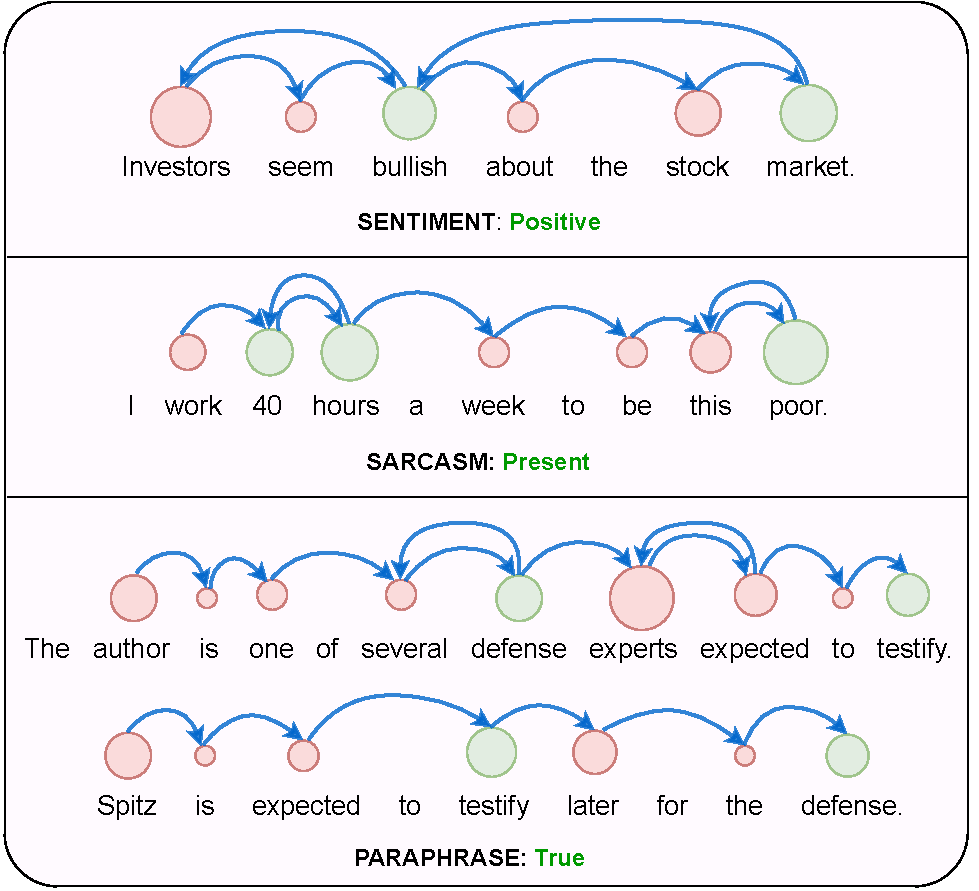
\includegraphics[width=1\columnwidth]{images/scanpath_sample_7.pdf}
    \caption{\small Generated scanpaths over text samples taken from various natural language processing (NLP) tasks. The green circles denote the important words characteristic of that task. The circles' size denotes the fixation duration, and the arrows depict the saccadic movements. As can be seen, linguistically important words often have a higher fixation duration and revisit. Regressions (word revisits) also appear in the examples. }
    \label{fig:scanpaths_for_NLP}
\end{figure}

Integrating human feedback in models can improve the performance of natural language processing (NLP) models. Feedback can be either explicit (\textit{e.g.} ranking used in training language models) or implicit (\textit{e.g.} using human cognitive signals in the form of eyetracking). Prior eye tracking and NLP research reveal that cognitive processes, such as human scanpaths, gleaned from human gaze patterns aid in the understanding and performance of NLP models. However, the collection of \textit{real} eyetracking data for NLP tasks is challenging due to the requirement of expensive and precise equipment coupled with privacy invasion issues. To address this challenge, we propose ScanTextGAN, a novel model for \textit{generating} human scanpaths over text. We show that ScanTextGAN-generated scanpaths can approximate meaningful cognitive signals in human gaze patterns. We include synthetically generated scanpaths in four popular NLP tasks spanning six different datasets as proof of concept and show that the models augmented with generated scanpaths improve the performance of all downstream NLP tasks.

\subsection{Introduction}
\label{sec:introduction-scantextgan}
Integrating human signals with deep learning models has been beginning to catch up in the last few years. Digital traces of human cognitive processing can provide valuable signals for Natural Language Processing \cite{klerke2016improving,plank-2016-keystroke}. Various approaches for integrating human signals have been explored. For example, human feedback for better decisioning \citep{christiano2017deep}, NLP tasks \citep{stiennon2020learning,wu2021recursively}, and most recently language modeling using reinforcement learning with human feedback (RLHF) based reward \citep{bai2022training,ouyang2022training}. RLHF involves explicit human feedback and is expensive and hard to scale. On the other hand, previous studies have also tried to use implicit human feedback in the form of eyetracking signals.
%, human eye gaze for computer vision tasks like image captioning and visual question answering \citep{he2019human,boyd2022human}, and NLP tasks like sentiment analysis and NER \citep{NoraNEREyeTracking}.
It has proven to be a useful signal for inferring human cognitive processing \cite{sood2020improving, hollenstein-zhang-2019-entity, ijcaiSurveyGapIdentified}. NLP researchers have focused on assessing the value of gaze information extracted from large, mostly dis-jointly labeled gaze datasets in recurrent neural network models \cite{ren-xiong-2021-cogalign,strzyz-etal-2019-towards,barrett-etal-2018-sequence}. The proposed approaches under this paradigm include gaze as an auxiliary task in multi-task learning \cite{klerke-etal-2016-improving,hollenstein2019advancing}, as additional signals \cite{mishra-etal-2016-harnessing}, as word embeddings \cite{barrett-etal-2018-unsupervised}, as type dictionaries \cite{barrett-etal-2016-weakly,hollenstein-zhang-2019-entity}, and
as attention \cite{barrett-etal-2018-sequence}. 

Previous studies demonstrate that human scanpaths (temporal sequences of eye fixations, see Fig.~\ref{fig:scanpaths_for_NLP}) gleaned from eye tracking data improve the performance of NLP models. However, the real-world application of these methods remains limited primarily due to the cost of precise eye-tracking equipment, users' privacy concerns, and manual labor associated with such a setup. Therefore, generating scanpaths from existing eyetracking corpora would add great value to NLP research. To the best of our knowledge, this is the first work to propose a model that generates scanpaths for a given read text with good accuracy. We call the model, ScanTextGAN.

\iffalse
    \begin{figure}[!t]
        %\vspace{-35mm}
        \centering
        \includegraphics[width=.9\columnwidth]{images/scanpath_sample_5.pdf}
        %\vspace{-8mm}
        \caption{\small A sample human scanpath, i.e., a temporal sequence of eye fixations and saccades over words in a sentence. The size of the circles denotes the fixation durations, and the arrows depict the saccadic movements. Regressions (word revisits) can also be recognized.}
        \label{fig:scanpath_sample}
        %\vspace{-5mm}
    \end{figure}
\fi


\begin{figure}[!t]
    % \vspace{-3mm}
    \centering
    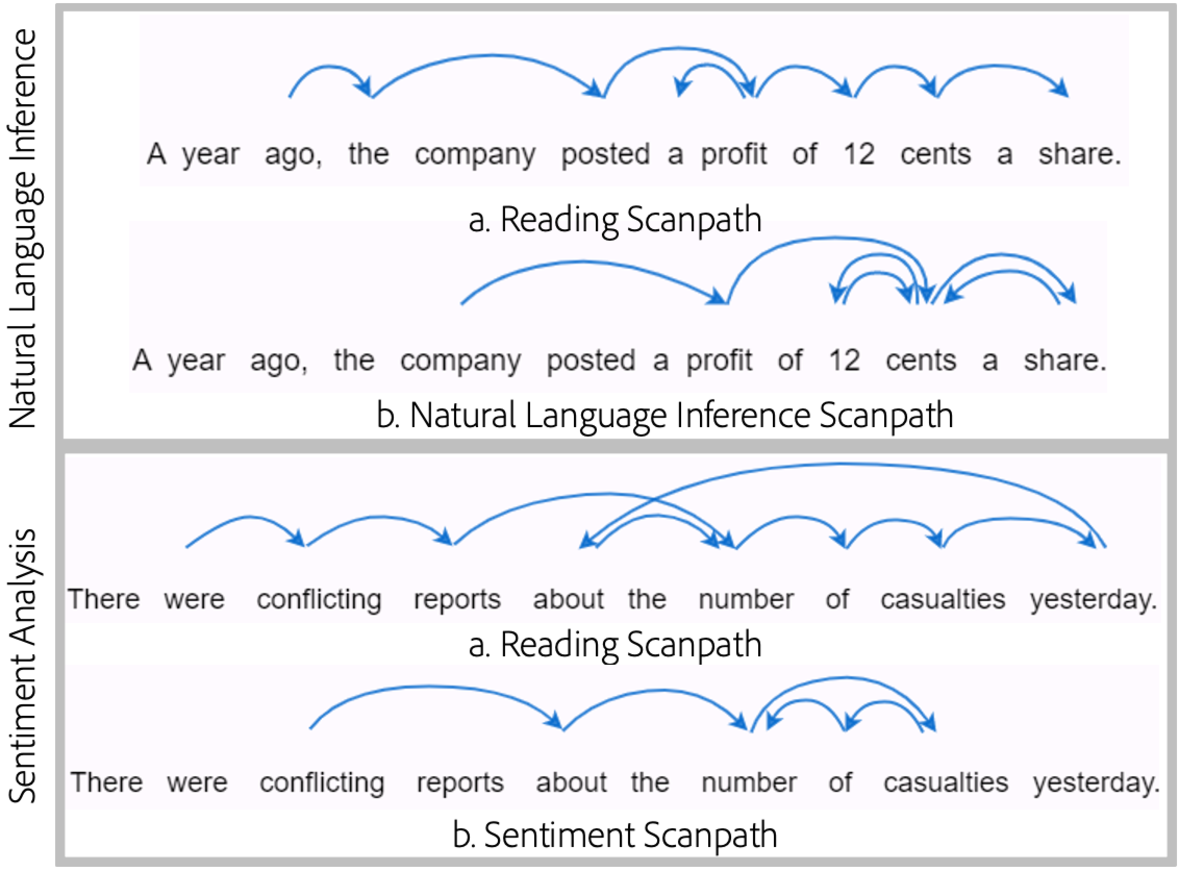
\includegraphics[width=0.7\columnwidth]{images/intent-scantextgan-scanpaths-3.pdf}
    %\vspace*{-2mm}
    \caption{\small (Intent-aware) Scanpath samples generated by conditioning scanpath generation on different downstream natural language tasks. Note that the conditioned scanpaths are heavily biased to words important for that downstream task.}
    \label{fig:intent-scanpaths-example} 
%\vspace{-3mm}
\end{figure}


We demonstrate the scanpath generation capability of ScanTextGAN over three eye-tracking datasets using multiple evaluation metrics. Further, we evaluate the utility of \textit{generated} scanpaths for improvements in the performance of multiple NLP tasks (see Figs.~\ref{fig:scanpaths_for_NLP},\ref{fig:intent-scanpaths-example}) including the ones in the GLUE benchmark \cite{wang-etal-2018-glue}. The generated scanpaths achieve similar performance gains as the models trained with real scanpaths for classic NLP tasks like sentiment classification, paraphrase detection, entailment, and sarcasm detection. 

Our contributions are threefold:

\noindent \textbf{1.} We propose ScanTextGAN, the first scanpath generator over text. \\
\textbf{2.} We compare ScanTextGAN with multiple baselines and conduct ablation experiments with varying models and configurations. The model performs well on the test sets and cross-domain generalization on two additional eyetracking datasets belonging to different text domains.\\
\textbf{3.} We tested the usefulness of generated scanpaths in downstream NLP tasks such as sentiment analysis, paraphrase detection, and sarcasm detection on six different datasets. The results show that the downstream NLP tasks benefited significantly from cognitive signals inherent in generated scanpaths. Further, we show how scanpaths change when finetuning with downstream natural language tasks (Figs.\ref{fig:intent-scanpaths-example},\ref{fig:intent-saliency-example}) and that they lead to further improvements in downstream task performance (\S\ref{sec:intent-scanpaths}) showing how they can act as additional controls beyond the task architecture.

% On six different datasets, we utilize the generated scanpaths to model downstream NLP tasks such as sentiment analysis, paraphrase detection, and sarcasm detection and show improved performance due to the cognitive signals contained in generated scanpaths. The results demonstrate that our model yields well-corroborated predictions with the human gaze on out-of-domain data.

%The rest of the paper is organized as follows. Section \ref{sec:RelatedWork} discusses the related work and identified research gap. Section \ref{sec:ProposedModel} illustrates the proposed model and datasets used for training, the training process, and loss functions, followed by Section \ref{sec:Performance Evaluation}, which summarizes the evaluation and discusses the results. Finally, Section \ref{sec:ConclusionFutureWork} concludes the paper considering possible future work.  




%%%%%%%%%%%%%%%%%%%%%%%%%%%%%%%%
\subsection{Related Work}
\label{sec:RelatedWork}

When reading a text, humans do not focus on every word and often do not read sequentially \cite{Just1980}. A series of studies in psycho-linguistics have shown that the number of fixations and the fixation duration on a word depend on several linguistic factors. The linguistic factors can also be determined given the cognitive features \cite{clifton2007eye, demberg2008data}.
Though advances in ML architecture have helped bring machine comprehension closer to human performance, humans are still superior for most NLP tasks \cite{blohm-etal-2018-comparing,xia-etal-2019-automatic}. 

It has been shown in the literature that integrating explicit \citep{bai2022training,ouyang2022training} and implicit (cognitive processing) human feedback signals in traditional ML models is expected to improve their performance \cite{Just1980}. However, the cost of explicit feedback (e.g., using MTurk) and implicit feedback (e.g., eye tracking) at scale is excessively high. Similarly, privacy-invasive eye-tracking processes limit the scope of this idea. One way to address this problem is to use generated eye movements to unfold the full potential of eye-tracking research. Hence, the idea is to architect ScanTextGAN, a scanpath generator for text reading, and test its usefulness in downstream NLP tasks. 

% Integrating human cognitive processing signals in traditional ML models is expected to improve performance \cite{Just1980}. However, the major hindrances is the unavailability and unacceptability of expensive and privacy-invasive eye-tracking process. One way to address this problem is to use generated eye movements to unfold the full potential of eye-tracking research. This motivated us to build the first scanpath generator for text, ScanTextGAN, and show its performance over both eye-tracking datasets and in downstream NLP tasks. Our work builds upon previous works on 1)~human attention modeling and 2)~gaze integration in neural network architectures.
More precisely, this work builds upon previous works on 1)~human attention modeling and 2)~gaze integration in neural network architectures, which are described as follows:

\textbf{Human Attention Modeling:} Predicting what people visually attend to in images (saliency prediction) is a long-standing challenge
in neuroscience and computer vision, the fields have seen many data-based models \cite{wang2021salient}. In contrast to images, most attention models for eye movement behaviors during reading are cognitive process models, \textit{i.e.}, models that do not involve machine learning but implement cognitive theories \cite{engbert2005swift,xia-etal-2019-automatic}. Key challenges for such models are a limited number of parameters and hand-crafted rules. Thus, it is difficult to adapt them to different tasks and domains and use them as part of end-to-end trained ML architectures \cite{kotseruba202040}. In contrast, learning-based attention models for text remain under-explored. Within that, all eye tracking models are saliency prediction models with non-existent work in predicting scanpaths. On the other hand, visual scanpaths generation for image-based eye tracking data has been recently explored for both traditional \cite{PathGANScanPathGen} and 360$^{\circ}$ images \cite{ScanGAN360}.

Matthies \textit{et al.} \cite{matthies-sogaard-2013-blinkers} presented the first fixation prediction work for text. They built a person-independent model using a linear Conditional Random Fields (CRF) model. %A separate line of work has instead tried incorporating assumptions about the human reading process into the model design. For \textit{e.g.}, 
Hahn and Keller \cite{hahn-keller-2016-modeling} designed the Neural Attention Trade-off (NEAT) language model, which was trained with hard attention and assigned a cost to each fixation. Other approaches include sentence representation learning using surprisal and part of speech tags as proxies to human attention \cite{10.5555/3171837.3171864}.%, attention as a way to improve time complexity for NLP tasks \cite{seo2018neural}, and learning saliency scores by training for sentence comparison \cite{samardzhiev-etal-2018-learning}.

Our work differs from previous studies as we combine cognitive theory and data-driven approaches to predict scanpaths and further show its application in downstream NLP tasks \cite{hollenstein-etal-2021-multilingual,hollenstein-etal-2021-cmcl}.




\textbf{Integrating Gaze in Network Architecture:} Integration of human gaze data into neural network architectures has been explored for a range of computer vision tasks such as image captioning, visual question answering, and tagging \cite{karessli2017gaze,yu2017supervising,he2019human,boyd2022human}. %In language processing, tracking a reader's eye movements provides information about the cognitive processes of text comprehension \cite{RaynerReadingComp, Just1980}. 
Hence, recent research has utilized features gleaned from readers' eye movement to improve the performance of complex NLP tasks such as sentiment analysis \cite{long-etal-2017-cognition, mishra-etal-2016-leveraging}, sarcasm detection \cite{mishra-etal-2016-harnessing}, part-of-speech tagging \cite{barrett-etal-2016-cross}, NER \cite{hollenstein-zhang-2019-entity}, and text difficulty \cite{ScanPathApp1}.

While in recent years, eye tracking data has been used to improve and evaluate NLP models, the scope of related studies remains limited due to the %one of the main limitations of these methods of cognitively-inspired NLP is the %limited availability of large datasets and the 
requirement of real-time gaze data at inference time. Mathias \textit{et al.} \cite{ijcaiSurveyGapIdentified} reported that there exists no automated way of generating scanpaths yet in the literature. With high-quality artificially generated scanpaths, the potential of leveraging eyetracking data for NLP can be unfolded. Additionally, generating scanpaths that mimic human reading behavior will help advance our understanding of the cognitive processes behind language understanding. Hence, we propose ScanTextGAN; researchers can use that to generate scanpaths over any text without worrying about collecting them from real users. 

%We show the utility of the generated scanpaths by achieving performance gains in downstream NLP tasks over six corpora.

\begin{landscape}
\begin{figure*}
%\vspace*{-12mm}
    \centering
    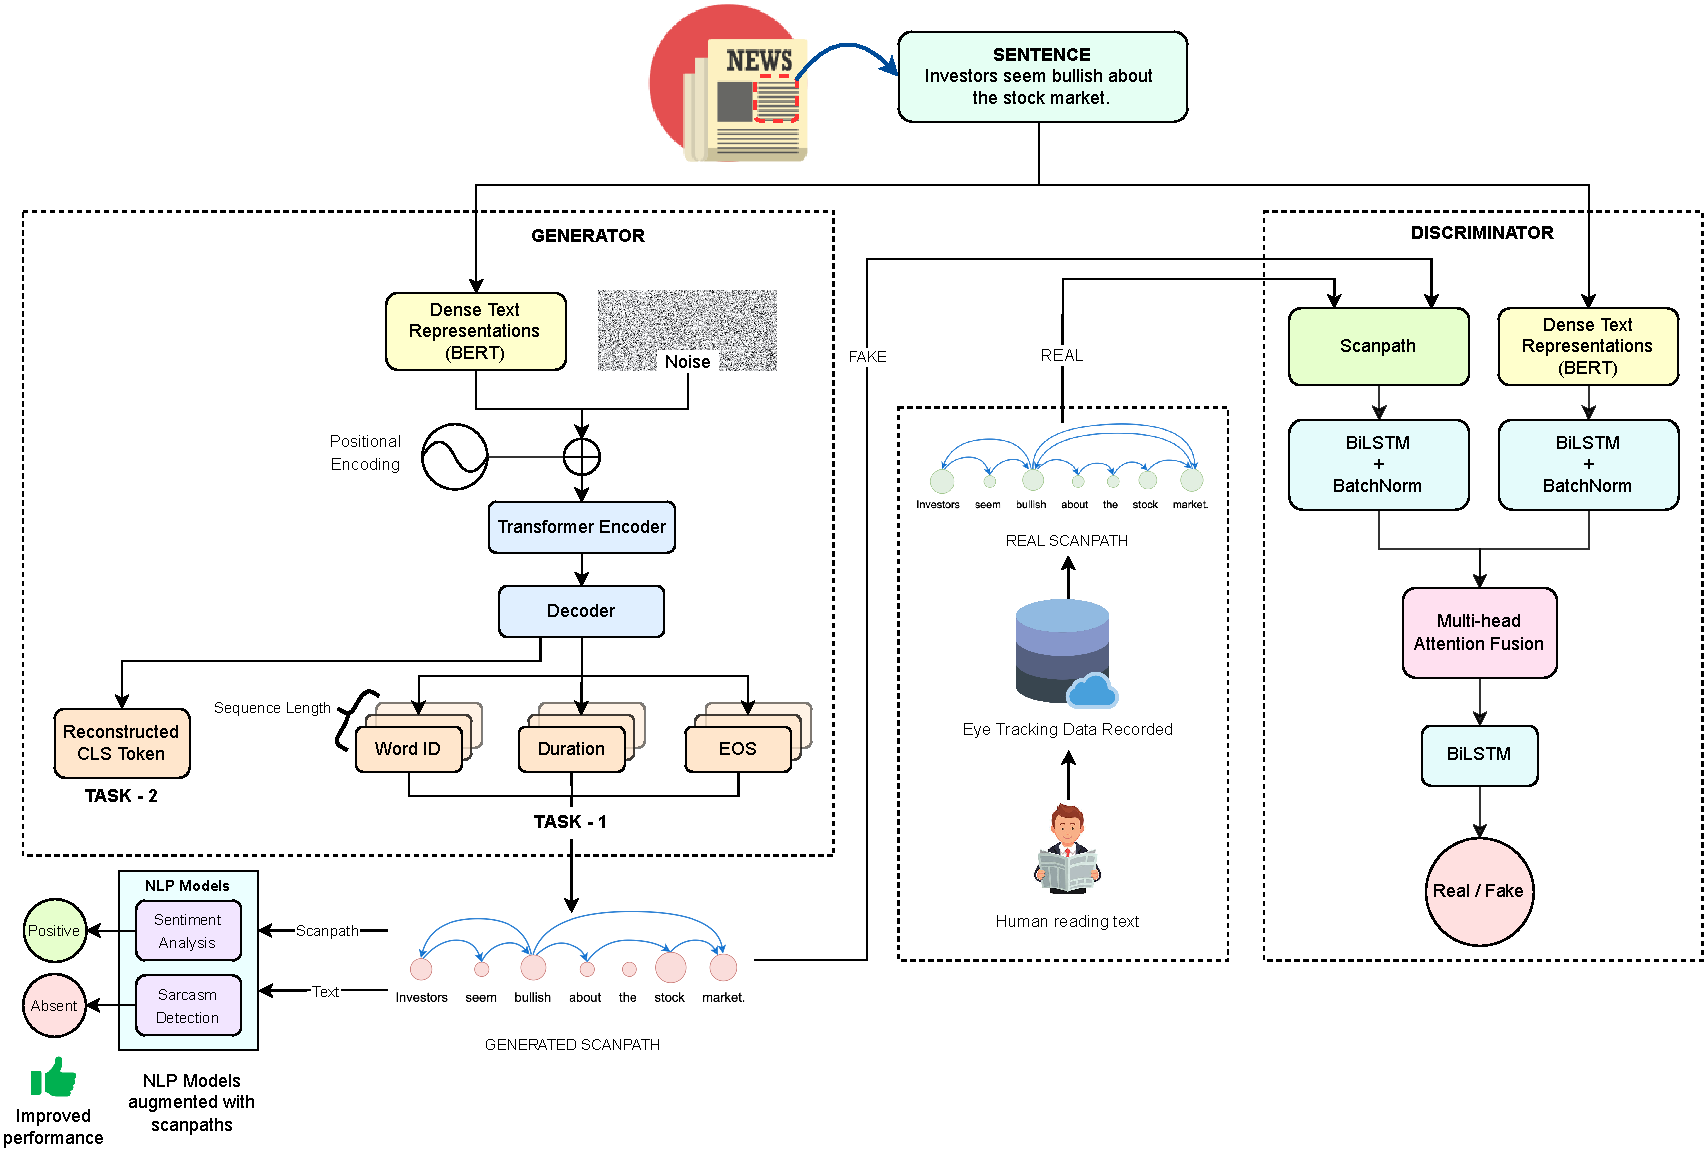
\includegraphics[width=1.2\textwidth]{images/scanpath_model_6.pdf}
    %\vspace*{-2mm}
    \caption{The architecture of the proposed \textbf{ScanTextGAN} model. The model consists of a conditional generator and a discriminator playing a zero-sum game. The generator is trained by two cognitively inspired losses: text content reconstruction and scanpath content reconstruction.}
    \label{fig:model} 
%\vspace*{-3mm}
\end{figure*}
\end{landscape}



\subsection{Proposed Model}
\label{sec:ProposedModel}
In this section, we define the scanpath generation task, describe the ScanTextGAN model architecture, and provide details on loss functions and model training.

\textbf{Task Definition:} The task of scanpath generation is to generate a sequence $\mathcal{S}(\mathcal{T})$ representing a scanpath over the text $\mathcal{T} = \{w_1,w_2,...,w_n\}$ composed of a sequence of words, can be defined as follows:
\begin{equation}
    \mathcal{S(T)} = \{..,(w_a^i,t^i),....,(w_b^j,t^j),....,(w_c^k,t^k)\}
\end{equation}
where $t^i$ represents the fixation duration over the word $w_a$ occurring at the position $i$.  Note that it is not necessary to have $a<b$ (words being read in linear order) or that $k=n$ (the number of fixations being equal to the number of words). Due to regressions, \textit{i.e.}, backward saccades to previous words, words are also revisited. Hence, the same word could appear multiple times in the sequence.

\subsubsection{ScanTextGAN Model Architecture}
Fig.~\ref{fig:model} illustrates the proposed conditional GAN architecture of the model. The ScanTextGAN model is composed of two competing agents. First, a conditional generator that generates scanpaths given text prompts. The second is a discriminator network, which distinguishes real human scanpaths from the generated ones. The ScanTextGAN model is trained by combining text content loss, scanpath content loss, and adversarial loss (Eq.~\ref{eq:Net Generator Loss}). The scanpath content loss measures the difference between the predicted scanpath and the corresponding ground truth scanpath. The text content loss reconstructs the input text, and the adversarial loss depends on the real/synthetic prediction of the discriminator over the generated scanpath. We describe the losses along with the generator and discriminator architectures next.

\looseness=-1 \textbf{Generator:} The ScanTextGAN generator constitutes a transformer-based encoder-decoder framework. The encoder is conditioned on BERT-based text embeddings \cite{devlin2018bert}, which are concatenated with noise to make the generator's output non-deterministic. The output of the transformer encoder is supplied to the decoder, which consists of task-specific feed-forward networks. One branch generates the scanpath (\textit{Task 1}), while the other reconstructs the $768$ dimensional CLS token embedding of the sentence (\textit{Task 2}). The scanpath is output as a temporal sequence of word ID (fixation points) $w_a^i$, fixation duration $t^i$, and end-of-sequence probability $EOS^i$. At inference time, the length $L(G)$ of generated scanpath $G$ is determined as follows:


\begin{equation}
L(G) = \begin{cases}
          \min_{1 \leq k \leq M} (k) \quad &\text{if} \, EOS^k > \tau \\
          M \quad &\text{otherwise} \, \\
     \end{cases}
\end{equation}
where $M$ is the maximum scanpath length as described in section \S\ref{sec:dataset} and $\tau \in (0,1)$ is a probability threshold. We use $\tau = 0.5$. The loss functions of the two branches are described below. 


\looseness=-1 \textbf{Scanpath Content Loss} tries to minimize the deviation of generated scanpaths $\mathcal{G}(\mathcal{T}, \mathcal{N})$ from the ground-truth scanpaths $\mathcal{R}(\mathcal{T}, h))$ over text $\mathcal{T}$ where ground-truth scanpaths are recorded from the human $h$ and $\mathcal{N}$ stands for Gaussian noise $\mathcal{N}(0, 1)$. The loss function $\mathbb{L}_s$ is given as:
\begin{equation}
    \label{eq:Scanpath Content Loss}
    \begin{aligned}
    \mathbb{L}_s(\mathcal{G}(\mathcal{T,}\mathcal{N}), \mathcal{R}(\mathcal{T},h)) = \frac{1}{k} \Sigma_{i=0}^{k}(&\alpha(id_g^i-id_r^i)^2 + \\ \beta(t_g^i-t_r^i)^2 + &\gamma (E_g^i-E_r^i)^2)
    % \\+ &\gamma P_g(E^i)*log(P_r(E^i)))
    \end{aligned}
\end{equation}
which is a weighted sum of three terms. The first term measures the error between real and predicted \textit{fixation points} given by the mean squared difference between generated and real word-ids $(id_g^i-id_r^i)$. It penalizes permutations of word ids and trains the model to approximate the real sequence of fixation points closely.

The second term measures the difference in \textit{fixation durations} given by the mean squared difference between generated and real duration $(t_g^i-t_r^i)$. Fixation durations simulate human attention over words in the input text. Thus, a word with a larger fixation duration is typically synonymous with greater importance than other words in the input text. This error term supplements the generator's ability to learn human attention patterns over the input text.

Finally, the third term measures the mean squared error between the prediction of end-of-sequence probability by real and generated distributions $(E_g^i-E_r^i)$. These are weighted by the hyperparameters $\alpha,\beta$, and $\gamma$. Preliminary experiments showed that optimizing the mean squared error leads to better performance over the cross-entropy loss for optimizing the EOS probability output.

\looseness=-1 \textbf{Text Content Loss:} Scanpaths depend heavily on the linguistic properties of the input text. Therefore, to guide the generator towards near the probable real data manifolds, we adopt reconstruction of the CLS token embedding of the input text (\textit{Task 2}) by the generator as an auxiliary task since the CLS token embedding encodes a global representation of the input text. 
This text content reconstruction loss $\mathbb{L}_r$ is given as: 
\begin{equation}
    \label{eq:Text Content Loss}
    \begin{aligned}
     \mathbb{L}_r(\mathcal{G}(\mathcal{T,}\mathcal{N}), \mathcal{R}(\mathcal{T},h)) = (&BERT(w_i^g,w_j^g,...,w_k^g\\-&BERT(w_a^r,w_b^r,...w_n^r))^2
    \end{aligned}
\end{equation}
where $BERT(w_a^r,w_b^r,...w_n^r)$ and $BERT(w_i^g,w_j^g,...w_k^g)$ stand for the \textit{CLS} vector representations of real and generated text respectively.

\textbf{Discriminator:} The goal of the discriminator is to distinguish between the real and synthetic scanpaths supplied to it. Similar to the generator, it requires text representations to distinguish between real and generated scanpaths. Specifically, the discriminator comprises two blocks of BiLSTMs that perform sequential modeling over the scanpaths and BERT embeddings. The outputs of the two branches are combined and passed to an attention fusion module with four heads, followed by another network of BiLSTMs. The hidden states of the last BiLSTM layer from both forward and backward directions are concatenated and supplied to a feed-forward network. A Sigmoid function activates the output of the feed-forward network. In this manner, the discriminator classifies the input scanpaths as either \textit{real} or \textit{fake}.

\textbf{Adversarial Loss:} The generator and discriminator networks are trained in a two-player zero-sum game fashion. The loss is given by:
\begin{equation}
    \label{eq:Adversarial Loss}
    \begin{aligned}
    \mathbb{L}_a = \min_{G}\max_{D}\mathbb{E}_{x\sim p_{\text{data}}(x)}[\log{D(x|\mathcal{T},h)}] + \\  \mathbb{E}_{z\sim p_{\text{z}}(z)}[1 - \log{D(G(z|\mathcal{T,N}))}]
    \end{aligned}
\end{equation}
Therefore, the net generator loss becomes:
\begin{equation}
    \label{eq:Net Generator Loss}
    \begin{aligned}
    \mathbb{L}_g = \mathbb{L}_s + \mathbb{L}_r + \mathbb{E}_{z\sim p_{\text{z}}(z)}[1 - \log{D(G(z|\mathcal{T,N}))}]
    \end{aligned}
\end{equation}

\subsubsection{Dataset} 
\label{sec:dataset}
\looseness=-1 For training the ScanTextGAN model, we use the CELER dataset \cite{berzak2022celer}. It contains eyetracking data of 365 participants for nearly 28.5 thousand newswire sentences, sourced from the Wall Street Journal Penn Treebank \cite{marcinkiewicz1994building}. Each participant in CELER reads 156 newswire sentences. Half of the sentences are shared across participants, and the rest is unique to each participant. The maximum sentence length was set to 100 characters. Participant eyetracking data were recorded using Eyelink 1000 tracker in a desktop mount configuration with a sampling rate of 1000 Hz. The ScanTextGAN model is trained to approximate the average eye movements of all the participants who read given sentences. The CELER dataset was envisioned to enable research on language processing and acquisition and to facilitate interactions between psycholinguistics and natural language processing. Furthering the goal, we use it to train our conditional GAN model through which we show human scanpath approximation capabilities (\S\ref{sec:Evaluation of Scanpath Generation}). Also, we use it to show improvements in the performance of NLP tasks (\S\ref{sec:Application to NLP Tasks}). 

\looseness=-1
The data consist of tuples of participant ID, sentence ID, and word ID corresponding to fixation point and fixation duration. We compute the 99th percentile of fixation durations and treat it as the largest value. Fixations of durations longer than this are treated as outliers and hence dropped from the dataset. To apply the scanpath reconstruction loss (Eq.~\ref{eq:Scanpath Content Loss}), we scale all fixation durations by the maximum value and then normalize them to [0,1]. Similarly, word IDs in each sentence are normalized to [0, 1] after scaling them by the length of that sentence. For the last fixation point in every scanpath, the binary EOS token is set to 1. The maximum scanpath length is set to 80 fixation points (99th percentile of the lengths). Thus shorter scanpaths are padded while longer scanpaths are trimmed. We use BERT to encode the sentences and obtain their $768$-dimensional embeddings, keeping the max length parameter as 80, thus resulting in an $80\times768$ dimensional tensor.

\subsubsection{Parameter Settings}
\looseness=-1
Sinusoidal positional encoding is applied over the input embeddings fed to the generator. We use a 3-layer transformer encoder with four head attention and a hidden dimension size of 776 in the generator. In the discriminator, we use bidirectional LSTMs over sentence embeddings and generated scanpaths with a hidden size of 64 and a dropout ratio of 0.3, followed by batch normalization for faster convergence. An attention module with four attention heads is applied after concatenating the outputs.
We employ the Adam and RMSProp optimizer to minimize generator and discriminator losses. The batch size is set to 128, the initial learning rate of the generator to 0.0001, and that of the discriminator to 0.00001. The model is trained for 300 epochs. Our implementation uses PyTorch, a popular deep-learning framework in Python. All experiments are run on an Intel Xeon CPU with Nvidia A100-SXM GPUs.



\subsection{Performance Evaluation}
\label{sec:Performance Evaluation}
We quantify the performance of ScanTextGAN in two regimes\footnote{All results are calculated with five random seeds and reported as the mean of those five runs}; first, scanpath generation with three datasets, and second, NLP tasks with six datasets. Similar to prior computer vision studies \cite{sun2019visual,de2022scanpathnet,kummerer2021state,jiang2016learning}, we evaluate the ScanTextGAN model over the scanpath generation task. For this, we use the test split of the CELER dataset, Mishra \textit{et al.} (2016) \cite{mishra2016predicting}, and Mishra \textit{et al.} (2017) \cite{Mishra_Kanojia_Nagar_Dey_Bhattacharyya_2017}. In addition, unlike the computer vision studies, we also evaluate the ScanTextGAN model for improvement in NLP tasks. The hypothesis is that the human eyes (and consequently the brain) process many language comprehension tasks unconsciously and without visible effort. The next logical step is to capture (or, in our case, generate) this mental representation of language understanding and use it to improve our machine-learning systems. For evaluation, we use four tasks from the GLUE benchmark and two from the tasks proposed by \cite{mishra2016predicting}. While the ScanTextGAN model is trained over news text from the CELER dataset, with the help of the other datasets, we expand our testing to other domains, including reviews, quotes, tweets, and Wikipedia text. 


\subsubsection{Evaluation Datasets}
\label{sec:eval_datasets}
\textbf{Mishra \textit{et al.} (2017) \cite{Mishra_Kanojia_Nagar_Dey_Bhattacharyya_2017}} comprises eye movements and reading difficulty data recorded for 32 paragraphs on 16 different topics, \textit{viz.} history, science, literature, \textit{etc}. For each topic, comparable paragraphs were extracted from Wikipedia\footnote{\url{https://en.wikipedia.org/}} and simple Wikipedia\footnote{\url{https://simple.wikipedia.org/}}. The participant's eye movements are tracked using an SR-Research Eyelink-1000 Plus eye tracker. Using the ground truth scanpaths over the text corpora, we evaluate the quality of generated scanpaths.


\textbf{Mishra \textit{et al.} (2016) \cite{mishra2016predicting}} contains eye fixation sequences of seven participants for 994 text snippets annotated for sentiment and sarcasm. These were taken from Amazon Movie Corpus %\cite{pang-lee-2004-sentimental}
, Twitter, and sarcastic quote websites. %They used an SR-Research Eyelink-1000 eye-tracker to collect the eye movements of the participants. 
The task assigned to the participants was to read one sentence at a time and annotate it with binary sentiment polarity labels (\textit{i.e.}, positive/negative). %Using feature engineering approaches, 
%They used the scanpath data to show improvements in sarcasm detection. 
The same datasets were used in several studies \cite{joshi-etal-2015-harnessing,mishra-etal-2016-harnessing,mishra-etal-2016-leveraging} to show improvements in sarcasm and sentiment analysis.
We use the datasets to evaluate both the generation quality and potential improvements in NLP tasks.% using generated scanpaths, thereby making it more aligned with real-world settings and solving the problem of the unavailability of human scanpath data at inference time.


\begin{table*}[!t]\centering
% \scriptsize
\resizebox{\textwidth}{!}{\begin{tabular}{lcccccc}\toprule
\multirow{2}{*}{\textbf{Generator Model}} &\multicolumn{4}{c}{\textbf{MultiMatch $\uparrow$}} &\multirow{2}{*}{\textbf{\makecell{Levenshtein\\Distance $\downarrow$}}} \\\cmidrule{2-5}
&\textbf{Vector$\uparrow$} &\textbf{Length$\uparrow$} &\textbf{Position$\uparrow$} &\textbf{Duration$\uparrow$} & \\\midrule
Inter-subject score\footnotemark & 0.973   & 0.958 &    0.830   & 0.698 & 0.691\\\midrule
%Transformer Encoder-Decoder &0.974 &0.958 &\textbf{0.819} &0.543 & \\
%Transformer Encoder &0.974 &0.957 &0.773 &0.703 & \\
\makecell[l]{LSTM Encoder-Decoder trained\\with scanpath content loss} & 0.975 & 0.956 &  0.765 & 0.344 & 0.865\\
\makecell[l]{ScanTextGAN -- Text \\Reconstruction -- GAN Loss}& 0.968 & 0.947 & 0.728 & 0.703 & 0.779\\
\textbf{ScanTextGAN} &\textbf{0.983} &\textbf{0.972} & \textbf{0.787} & 0.733 & \textbf{0.769}\\
ScanTextGAN -- Text Reconstruction &0.974 &0.957 &0.773 &0.703 & 0.798\\
ScanTextGAN -- GAN Loss &0.973 &0.955 &0.750 &\textbf{0.761} &0.786\\
% *ScanTextGAN + Dwell Time reconstruction & 0.960 & 0.932 & \textbf{0.805} & 0.711 \\
% *Dwell Time reconstruction w/o Adv. training & 0.966 &0.939	&0.786 &0.775 \\
ScanTextGAN + addition of noise &0.971 &0.952 &0.756 &0.736 &0.791\\
\makecell[l]{ScanTextGAN -- Text (CLS) \\Reconstruction + sentence reconstruction} &0.978 &0.963 &0.724 &0.721 &0.805 \\
% \midrule
% Inter-Subject Scanpath Topline & XXX & & & & 
% \\ 
\bottomrule
\end{tabular}}
\caption{In-domain Evaluation of Scanpath Generation on the CELER dataset \cite{berzak2022celer}.}\label{tab:celer}
\end{table*}


\footnotetext{In the CELER dataset, there are only 78 shared sentences amongst all the participants. Therefore, inter-subject scanpath evaluation is done only for these sentences. In contrast, the ScanTextGAN results are reported for the entire test set (including these 78 sentences).}


Furthermore, we explore the potential of including cognitive signals contained in scanpaths in NLP models for a range of GLUE tasks which include Sentiment Analysis using Stanford Sentiment Treebank (SST), Paraphrase Detection using Microsoft Research Paraphrase Corpus (MRPC) and Quora Question Pairs (QQP), Natural Language Inference using Recognizing Textual Entailment (RTE) dataset.
%- \textbf{SST}: The Stanford Sentiment Treebank includes fine-grained sentiment labels for 215154 phrases in the parse trees of 11855 sentences. The corpus consists of sentences from movie reviews and human sentiment annotations. The task is to predict the sentiment of a given sentence. We use the two-way (positive/negative) class split and only sentence-level labels.\\
%- \textbf{MRPC}: The Microsoft Research Paraphrase Corpus comprises a set of 5,801 sentence pairs collected from newswire articles. Each pair is annotated with a label indicating whether the sentences are paraphrased or not.\\
% Each pair is labeled whether human annotators paraphrase it. The dataset is divided into \textit{train} (4,076 sentence pairs, of which 2,753 are paraphrases) and \textit{test} (1725 pairs, of which 1,147 are paraphrases).\\
%- \textbf{QQP}: The Quora Question Pairs (QQP) dataset consists of over 400,000 question pairs. Each is annotated with a binary value indicating whether the two questions are paraphrases of each other. \\
%- \textbf{RTE}: The Recognizing Textual Entailment (RTE) dataset involves a generic Natural Language Inference task that recognizes, given a pair of texts, whether the meaning of one text can be inferred from the other. 

Next, we cover the results of scanpath generation and its application in NLP tasks.



\begin{figure}[]
    \centering
    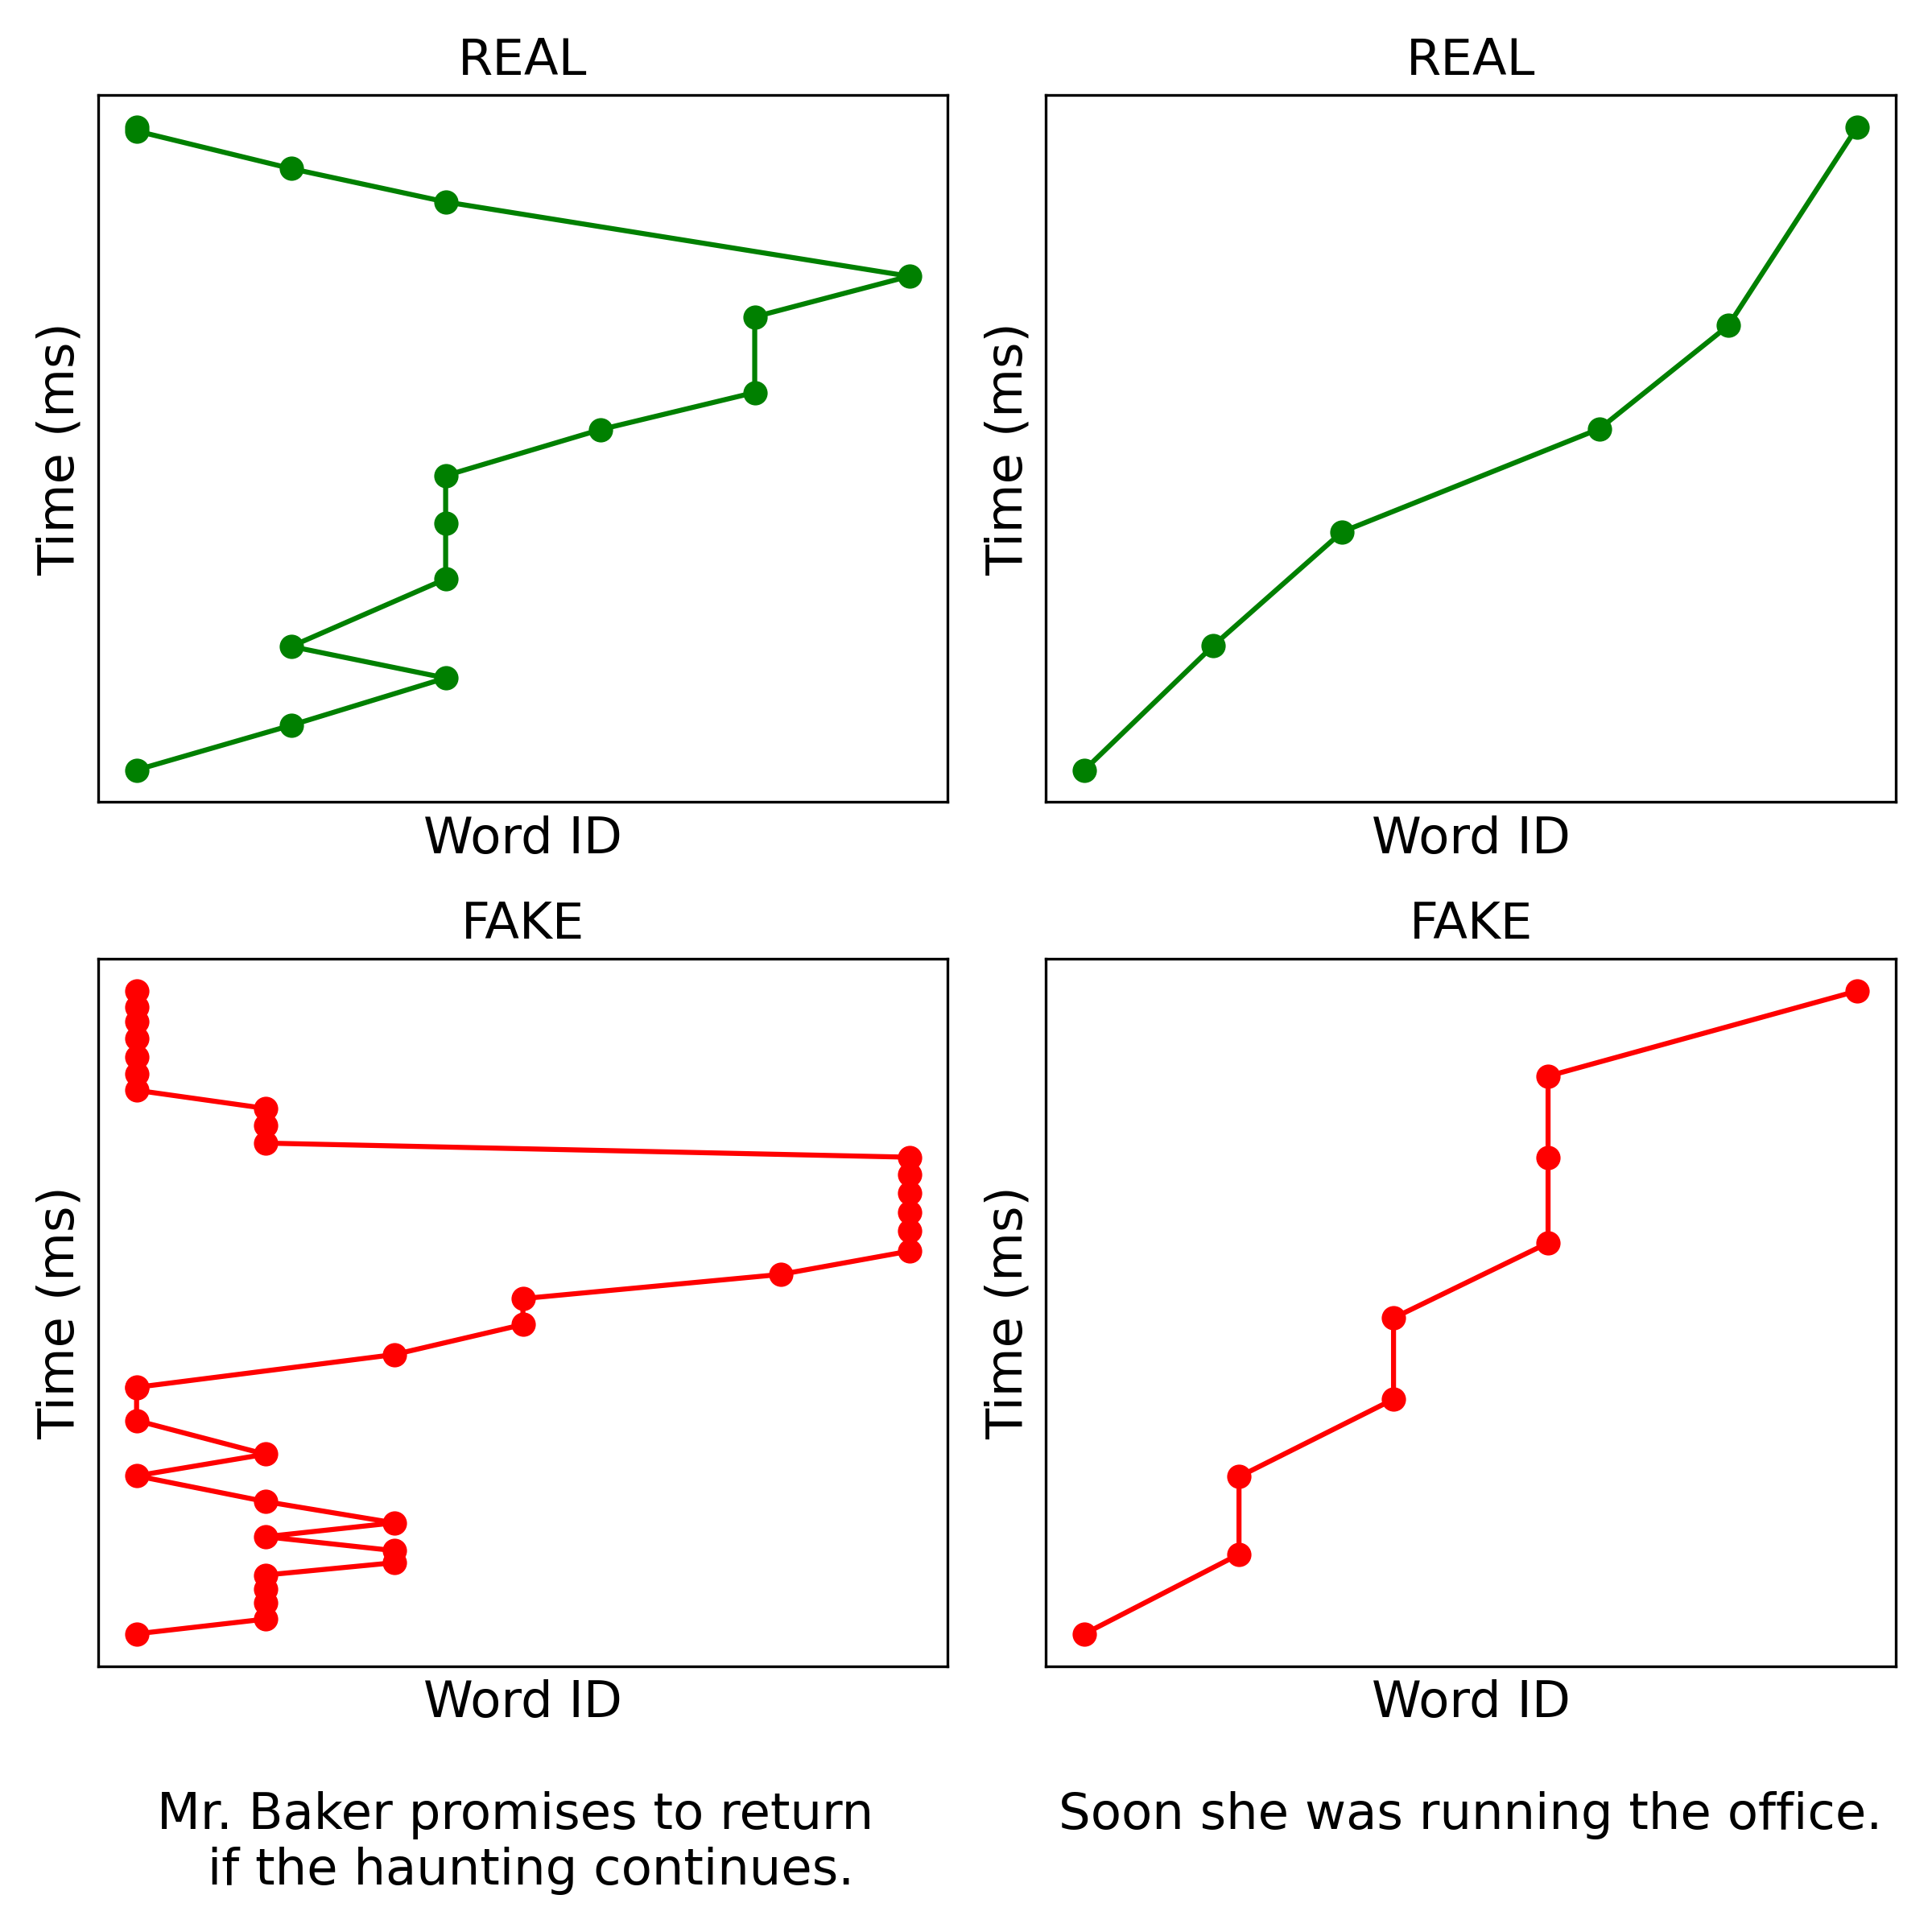
\includegraphics[width=0.9\columnwidth]{images/scanpath_plot_combined_sent_5.png}
    \caption{Comparison of \textit{real} and \textit{synthesized} scanpaths corresponding to a few text samples. The proposed ScanTextGAN model generates the latter.}
    \label{fig:scanpath_comparison}
\end{figure}


\subsubsection{Evaluation of Scanpath Generation}
\label{sec:Evaluation of Scanpath Generation}
We evaluate the scanpath generation model on two most commonly used metrics in image scanpath generation studies \cite{sun2019visual,chen2018scanpath,de2022scanpathnet,kummerer2022deepgaze}: \textbf{MultiMatch} \cite{jarodzka2010vector} and \textbf{Levenshtein Distance} \cite{levenshtein1965leveinshtein}. Multimatch is a geometrical measure that compares scanpaths across a comprehensive set of dimensions composed of shape, lengths, position, and fixation duration. Levenshtein Distance between a pair of sequences measures the least number of edits (inserts, deletes, substitution) to transform one into the other.

\paragraph{Scanpath Evaluation Metrics}
\label{sec:appendix_scanpath_metrics}

\textbf{MultiMatch} is a geometrical measure that models scanpaths as vectors in 2-D space, wherein the vectors represent saccadic eye movements. Starting and ending coordinates of these saccades constitute the fixation positions. It compares scanpaths across multiple dimensions, \textit{viz.} shape, length, position, direction, and fixation duration. Shape measures the vector difference between aligned saccade pairs, which is then normalized by twice the diagonal screen size. Length measures the normalized difference between the endpoints of real and generated saccade vectors. Direction is the angular distance between the two vectors. The position is the Euclidean difference in position between aligned vectors, and duration measures the difference in fixation durations normalized against the maximum duration. Since our work deals with scanpaths over text, we use 1-D space to represent the saccade vectors where word IDs denote the fixation positions. Thus, it is easy to see that computing scanpath direction similarity is redundant here (it is subsumed within position); hence we drop it from our analysis. 


\textbf{Levenshtein Distance} between a pair of sequences measures the least number of character edits, i.e., insertion, deletion, and substitution needed to transform one sequence into the other.
Specifically, we use it to gauge the degree of dissimilarity between a pair of real $R$ and generated $G$ scanpaths. To account for the fixation durations of each word, $R$ and $G$ are temporally binned using a $50$ ms bin size, similar to the computation of ScanMatch metric \cite{cristino2010scanmatch}. The resulting sequences of word IDs, $R_W$ and $G_W$ are transformed into character strings, $R_S = \{r_1, r_2, ..., r_n\}$ and $G_S = \{g_1, g_2, ...,g_m\}$, where $R_S$ and $G_S$ are strings over the ASCII alphabet and $n = |R_S|$ and $m = |G_S|$.
Thus, a lower NLD score is indicative of greater scanpath similarity. 


Further, as a top-line comparison, we use \textbf{inter-subject scanpath similarity} \cite{sun2019visual}. It measures the degree of variation among real human scanpaths corresponding to each text input. To compute this, we first calculate each subject's performance by treating the scanpaths of other subjects as the ground truth. Then, the average value of all subjects is used as inter-subject performance.


\textbf{Baselines:} Since ScanTextGAN is the first text-based scanpath generation model, we conduct an ablation study to compare ScanTextGAN with its other variants. Specifically, we compare ScanTextGAN with the following six configurations: (1)~An LSTM-based network trained with scanpath content loss. Sentence embeddings obtained through BERT are concatenated with noise in this model. The resultant is fed to an attention module with four heads, then passed to a network of LSTMs and Batch Normalization layers applied in tandem. (2)~ScanTextGAN model trained with only the scanpath content loss. (3)~ScanTextGAN model without the text reconstruction loss (Task-2). (4)~ScanTextGAN model with BERT-based sentence embeddings reconstruction instead of CLS token reconstruction. (5)~ScanTextGAN model with the addition of noise instead of concatenation. (6)~ScanTextGAN model trained without GAN loss.



\begin{table*}[!t]\centering
% \scriptsize
\resizebox{\textwidth}{!}{\begin{tabular}{lcccccc}\toprule
\multirow{2}{*}{\textbf{Generator Model}} &\multicolumn{4}{c}{\textbf{MultiMatch $\uparrow$}} &\multirow{2}{*}{\textbf{\makecell{Levenshtein\\Distance $\downarrow$}}} \\\cmidrule{2-5}
&\textbf{Vector$\uparrow$} &\textbf{Length$\uparrow$} &\textbf{Position$\uparrow$} &\textbf{Duration$\uparrow$} & \\\midrule
Inter-subject score & 0.977   & 0.963 &    0.839   & 0.715 & 0.723\\\midrule
\makecell[l]{LSTM Encoder-Decoder trained\\with scanpath content loss}& \textbf{0.984}    & \textbf{0.973} &   0.714 &   0.379 & 0.918\\
\makecell[l]{ScanTextGAN -- Text\\Reconstruction -- GAN Loss}& 0.977   & 0.960 &    0.780   & 0.769 & 0.847\\
%Transformer Encoder-Decoder &0.977 &0.957 &0.821 &0.574 & \\
%Transformer Encoder &0.976 &0.961 &0.763 &0.757 & \\
\textbf{ScanTextGAN} &0.966 &0.945 &\textbf{0.791} &\textbf{0.771} & \textbf{0.836} \\
ScanTextGAN -- Text Reconstruction &0.976 &0.961 &0.763 &0.757 & 0.845\\
% *ScanTextGAN + Dwell Time reconstruction & 0.971 &0.952 & \textbf{0.797} &0.711 \\
% *Dwell Time reconstruction w/o Adv. training & 0.976 &0.959	&0.795 &0.765 \\
ScanTextGAN -- GAN Loss &0.976 &0.959 &0.774 &0.768 &0.839\\
ScanTextGAN + addition of noise &0.968 &0.947 &0.737 &0.743 & 0.838\\
\makecell[l]{ScanTextGAN -- Text (CLS) \\Reconstruction + sentence reconstruction}&0.964 &0.934 &0.747 &0.733 & 0.869\\
\bottomrule
\end{tabular}}
\caption{Cross-domain Evaluation of Scanpath Generation on the Dataset by \cite{mishra2016predicting}.}\label{tab:iitb_2016}
%\vspace*{-3mm}
\end{table*}

\begin{table*}[!t]\centering
% \vspace*{-10mm}
% \scriptsize
\resizebox{\textwidth}{!}{\begin{tabular}{lcccccc}\toprule
\multirow{2}{*}{\textbf{Generator Model}} &\multicolumn{4}{c}{\textbf{MultiMatch $\uparrow$}} &\multirow{2}{*}{\textbf{\makecell{Levenshtein\\Distance $\downarrow$}}} \\\cmidrule{2-5}
&\textbf{Vector$\uparrow$} &\textbf{Length$\uparrow$} &\textbf{Position$\uparrow$} &\textbf{Duration$\uparrow$} & \\\midrule
Inter-subject score & 0.994   & 0.991 &    0.834   & 0.620 & 0.845\\\midrule
\makecell[l]{LSTM Encoder-Decoder trained\\with scanpath content loss}& \textbf{0.992}  &  \textbf{0.987}   & 0.596 &    0.329 & 0.969\\
\makecell[l]{ScanTextGAN -- Text\\Reconstruction -- GAN Loss}&0.990 &0.984 &0.729 &0.705 & 0.951\\
%Transformer Encoder &0.986 &0.981 &0.776 &0.706 & \\
\textbf{ScanTextGAN} &0.984 &0.977 &\textbf{0.759} &0.693 & \textbf{0.931}\\
ScanTextGAN -- Text Reconstruction &0.986 &0.981 &0.756 &\textbf{0.706} & 0.939\\
% *ScanTextGAN + Dwell Time reconstruction & 0.985 &0.977	&\textbf{0.773}	&0.605 \\
% *Dwell Time reconstruction w/o Adv. training &0.990	&0.985 &0.686	&0.701 \\
ScanTextGAN -- GAN Loss &0.990 &0.984 &0.739 &\textbf{0.706} &0.945\\
ScanTextGAN + addition of noise &0.984 &0.976 &0.759 &0.703 & 0.943\\
\makecell[l]{ScanTextGAN -- Text (CLS) \\Reconstruction + sentence reconstruction} &0.983 &0.974 &0.667 &0.674 & 0.958\\
\bottomrule
\end{tabular}}
\caption{Cross-domain Evaluation of Scanpath Generation on the Dataset by \cite{Mishra_Kanojia_Nagar_Dey_Bhattacharyya_2017}.}\label{tab:iitb_2017}
%\vspace*{-3mm}
\end{table*}



\textbf{Results:} Table~\ref{tab:celer} presents the results of our scanpath prediction model on the CELER dataset. Further, we also compare ScanTextGAN with baselines on two other contemporary datasets of movie reviews, tweets, and sarcastic quotes \cite{mishra2016predicting},  Wikipedia and simple Wikipedia paragraphs  \cite{Mishra_Kanojia_Nagar_Dey_Bhattacharyya_2017}. Tables~\ref{tab:iitb_2016} and \ref{tab:iitb_2017} present the results of our model on those datasets. For obtaining results on these corpora, we use the model trained on the CELER dataset, thus helping us evaluate the cross-domain performance of the model. 

As can be seen in Table~\ref{tab:celer}, Table~\ref{tab:iitb_2016} and Table~\ref{tab:iitb_2017}, ScanTextGAN outperforms other models for scanpath prediction on most metrics. The performance of ScanTextGAN even surpasses inter-subject reference on Duration and comes very close to Vector, Length, and Position. 

We observe that adopting the reconstruction of the CLS token as an auxiliary task (Task - 2) boosts the model performance. Reconstructing the full sentence embeddings rather than the CLS tokens only as an auxiliary task does not always improve the results, despite adding a larger computational overhead. The results also reveal that concatenating noise with text embeddings is more rewarding than adding it.

Further, to compare the skipping behavior of ScanTextGAN with humans, we calculate the weighted F1 score of the words skipped and attended by both model types. We find the weighted F1 to be 64.6 between them. Fig.~\ref{fig:scanpath_comparison} presents a visual comparison between real scanpaths from the available eyetracking data and scanpaths generated by ScanTextGAN, corresponding to some randomly chosen text samples. We can observe that the generated scanpaths resemble the real ones to a great extent. Thus, the quantitative and qualitative results on in-domain and cross-domain settings lead us to believe that our proposed scanpath generation model can be deemed a good approximator of the human scanpaths. % and can be used for downstream NLP applications.


%%%%%%%%%%%%%%%%%%%%%%%%%%%%%%%%%%%%%%%%%%%%%%%%%%%%%%%%%%%%%%%%%%
%%%%%%%%%%%%%%%%%%%%%%%%%%%%%%%%%%%%%%%%%%%%%%%%%%%%%%%%%%%%%%%%%%
\subsubsection{Application to NLP Tasks}
\label{sec:Application to NLP Tasks}
% \begin{table}[t]\centering
% \caption{Sentiment analysis and sarcasm detection results on the dataset by \cite{mishra2016predicting}. Model configuration refers to the type of scanpath included in train and test data.}
% \label{tab:iitb_classifier_results}
% % \scriptsize
% \begin{tabular}{cc|ccc}\toprule
% \multicolumn{2}{c}{\textbf{Model Configuration}} &\multicolumn{2}{c}{\textbf{Weighted F1 score}} \\\cmidrule{1-4}
% \textbf{Train} & \textbf{Test} &\textbf{Sentiment} &\textbf{Sarcasm} \\\midrule
% None &None &0.7839 &0.9438 \\
% Real &Real &0.8334 &0.9501 \\
% Random &Generated &0.7773 &0.9313 \\
% Real &Generated &0.8319 &0.9378 \\
% Generated &Real &0.8402 &0.9452 \\
% Generated &Generated &0.8332 &0.9506 \\
% Real+Generated &Generated &\textbf{0.8404} &\textbf{0.9512} \\
% \bottomrule
% \end{tabular}
% \end{table}

% \usepackage{booktabs}

We use them to augment various NLP models and measure their performance to demonstrate the usefulness of cognitive signals hidden in the \textit{generated} scanpaths.

\textbf{Sentiment Classification and Sarcasm Detection:} For these tasks, we use a model consisting of a network of two branches of BiLSTMs and Batch Normalization layers that perform sequential modeling over text representations obtained through BERT and scanpaths fed as input to the model. The outputs of both branches are combined and passed to another layer of BiLSTMs, followed by a feed-forward network that predicts binary sentiment/sarcasm labels corresponding to the input after activating with the Sigmoid function. We follow a 10-fold cross-validation regime.

We compare the models with generated scanpaths, real scanpaths, and without scanpaths. Further, to investigate whether performance gains observed by adding scanpaths are due to scanpaths and not the increase in the number of parameters, we train a \textit{Random-Random} variant in which we send Random noise as scanpaths to the model with an increased number of parameters. We also simulate the real-world case where both real and generated scanpaths are available during train time, but only generated ones are available during test time, for example, during user deployment. 
%We also compare the results for all tasks with models fed with random noise as scanpaths. 
\begin{table}[!t]
\centering
% \vspace{-10mm}
\begin{tabular}{llcc} 
\toprule
\multicolumn{2}{c}{\textbf{Model Configuration}} & \multicolumn{2}{c}{\textbf{F1 score}}  \\ 
\midrule
\textbf{Train}   & \textbf{Test}                 & \textbf{Sentiment} & \textbf{Sarcasm}           \\ 
\midrule
w/o              & w/o                           & 0.7839             & 0.9438                     \\
Random           & Random                     & 0.7990             & 0.9397    \\
Random           & Generated                     & 0.7773             & 0.9313                     \\
Real             & Generated                     & 0.8319             & 0.9378                     \\
Real      & Real        & 0.8334        & 0.9501             \\
Generated        & Real                          & 0.8402             & 0.9452                     \\
Generated        & Generated                     & 0.8332             & 0.9506                     \\
Real + Generated & Generated                     & \textbf{0.8404}    & \textbf{0.9512}            \\ \midrule

Intent-Aware & Intent-Aware & \textbf{0.8477} & \textbf{0.9528} \\ \bottomrule
\end{tabular}
\caption{Sentiment analysis and sarcasm detection results on the dataset by \cite{mishra2016predicting}. Model configuration refers to the type of scanpath included in train and test data.\label{tab:iitb_classifier_results}
}
%\vspace{-3mm}
\end{table}

Table~\ref{tab:iitb_classifier_results} records the results of sentiment analysis and sarcasm detection tasks \cite{mishra2016predicting}. We note that generated scanpaths training and testing lead to similar gains for sentiment analysis and sarcasm detection as real scanpaths. The model with an increased number of parameters fed random noise in place of scanpaths performs similarly to the model trained without any scanpaths. Interestingly, the best results are obtained when model training uses both real and generated scanpaths. We believe this is due to ScanTextGAN bringing additional cognitive information from the news-reading CELER corpus, which is not present in the real scanpaths in \cite{mishra2016predicting}. In addition to the intrinsic evaluation presented in \S\ref{sec:Evaluation of Scanpath Generation}, this downstream evaluation demonstrates the high quality of the synthesized scanpaths, showing that they contain valuable cognitive processing signals for NLP tasks.


\textbf{GLUE Tasks}:
To validate further, we augment classification models (based on sequential modeling using LSTMs) with generated scanpaths to show performance improvement in downstream NLP tasks on four GLUE benchmark datasets – SST, MRPC, RTE, QQP as described in \S\ref{sec:eval_datasets}.
% (Since our goal is to establish the hypothesis that scanpaths lead to performance improvement in NLP models and do not necessarily achieve state-of-the-art results, we use simple classification models.)
Table~\ref{tab:glue_results} reports the accuracy and weighted-F1 scores of the models trained with and without scanpaths for these tasks. We observe that in all four tasks, the model trained with generated scanpaths outperforms the one without scanpaths. 


% \begin{table}[!htp]\centering
% %\vspace{-2mm}
% \caption{\small Results on GLUE benchmark tasks.}\label{tab:glue_results}
% % \scriptsize
% \begin{tabular}{lccc}\toprule
% \textbf{Model} &\textbf{Acc} &\textbf{F1} \\\midrule
% \textit{Dataset} &\multicolumn{2}{c}{\textbf{SST}} \\\midrule
% Without scanpaths &0.8090 &0.8089 \\
% With generated scanpaths &\textbf{0.8138} &\textbf{0.8138} \\\midrule
% \textit{Dataset} &\multicolumn{2}{c}{\textbf{MRPC}} \\\midrule
% Without scanpaths &0.6902 &0.6656 \\
% With generated scanpaths &\textbf{0.6969} &\textbf{0.6828} \\\midrule
% \textit{Dataset} &\multicolumn{2}{c}{\textbf{RTE}} \\\midrule
% Without scanpaths &0.6162 &0.6080 \\
% With generated scanpaths &\textbf{0.6211} &\textbf{0.6205} \\
% \bottomrule
% \end{tabular}
% %\vspace{-2mm}
% \end{table}

\begin{table}[!t]
\centering
% \vspace{-10mm}
\begin{tabular}{llcc} 
\toprule
\textbf{Dataset}      & \textbf{Model}         & \textbf{Acc}    & \textbf{F1 score}  \\ 
\midrule
\multirow{2}{*}{SST}  & w/o scanpaths           & 0.8090           & 0.8089             \\
                      & w/ random scanpaths & 0.8059 & 0.8061  \\
                      
                      & w/ generated scanpaths & \textbf{0.8138} & \textbf{0.8138}  \\\cmidrule{2-4}
                      & w/ intent-aware scanpaths & \textbf{0.8269} &	\textbf{0.8272}
                      \\\midrule
\multirow{2}{*}{MRPC} & w/o scanpaths           & 0.6902          & 0.6656             \\
                      & w/ random scanpaths & 0.6623 & 0.6680  \\
                      & w/ generated scanpaths & \textbf{0.6969} & \textbf{0.6828}   \\\cmidrule{2-4}
                      & w/ intent-aware scanpaths & \textbf{0.7009} &	\textbf{0.6911}
                      \\\midrule
\multirow{2}{*}{RTE}  & w/o scanpaths           & 0.6162          & 0.6080              \\
                      & w/ random scanpaths & 0.5802 & 0.5794  \\
                      & w/ generated scanpaths & \textbf{0.6211} & \textbf{0.6205}   \\\cmidrule{2-4}
                      & w/ intent-aware scanpaths & \textbf{0.6293} &	\textbf{0.6278}
                      \\\midrule
\multirow{2}{*}{QQP}  & w/o scanpaths           & 0.8499          & 0.8513              \\
                    & w/ random scanpaths & 0.8491 & 0.8503  \\
                    & w/ generated scanpaths & \textbf{0.8578} & \textbf{0.8596}    \\\cmidrule{2-4}
                      & w/ intent-aware scanpaths & \textbf{0.8648} &	\textbf{0.8658} \\
\bottomrule
\end{tabular}
\caption{Results of training NLP models with and without scanpaths on the GLUE benchmark tasks. Including scanpaths leads to consistent improvements across all the NLP tasks.\label{tab:glue_results}}
%\vspace{-3mm}
\end{table}

\iffalse
    \begin{table*}[!h]\centering
    \caption{Results of Sentiment Analysis and Sarcasm Detection tasks on \cite{mishra2016predicting}}
    \label{tab:iitb_classifier_results}
    % \scriptsize
    \begin{tabular}{cccccccc}\toprule
    \multicolumn{5}{c}{\textbf{Model Configuration}} &\multicolumn{2}{c}{\textbf{Weighted F1 score}} \\\cmidrule{1-7}
    \multicolumn{3}{c}{\textbf{Train}} &\multicolumn{2}{c}{\textbf{Test}} &\multirow{2}{*}{\textbf{Sentiment Analysis}} &\multirow{2}{*}{\textbf{Sarcasm Detection}} \\\cmidrule{1-5}
    Generated &Real &Random &Generated &Real & & \\\midrule
    \xmark &\xmark &\xmark &\xmark &\xmark &0.7839 &0.9438 \\
    \xmark &\xmark &\cmark &\cmark &\xmark &0.7773 &0.9313 \\
    \cmark &\xmark &\xmark &\cmark &\xmark &0.8332 &0.9506 \\
    \xmark &\cmark &\xmark &\xmark &\cmark &0.8334 &0.9501 \\
    \xmark &\cmark &\xmark &\cmark &\xmark &0.8319 &0.9378 \\
    \cmark &\cmark &\xmark &\cmark &\xmark &\textbf{0.8404} &\textbf{0.9512} \\
    \bottomrule
    \end{tabular}
    \end{table*}
    
\fi
 
\textbf{Intent-Aware Scanpaths:} \label{sec:intent-scanpaths} Finally, we try to condition scanpaths generation on the downstream natural language task. We back-propagate gradients from the downstream NLP task to the conditional generator. In this fashion, the model learns to generate \textit{intent-aware} scanpaths.
The hypothesis is that finetuning scanpath generation based on feedback from the natural language task will bias the generator towards words more pertinent to that task and thus could help further improve performance on the downstream task. The architecture is shown in Fig~\ref{fig:intent-model}. The results in Tables~\ref{tab:iitb_classifier_results} and \ref{tab:glue_results} validate the hypothesis that we observe consistent improvements in all downstream tasks. Fig~\ref{fig:intent-scanpaths-example} and Fig~\ref{fig:intent-saliency-example} show a few examples of scanpaths and saliency generated for three downstream natural language tasks. 

Together these results corroborate the hypothesis that leveraging the cognitive signals approximated by synthetic scanpaths in NLP models leads to performance gains.



\subsection{Intent-Aware Scanpaths}
\label{sec:appendix_intent_aware_scanpaths}
As described in section \S\ref{sec:Application to NLP Tasks}, the generator conditioned on the downstream natural language task yields \textit{intent-aware} scanpaths. Augmenting NLP models with these scanpaths leads to higher performance gains. Here, we provide more details on \textit{intent-aware} scanpath generation.
Please refer to figures \ref{fig:intent-model} and \ref{fig:intent-saliency-example} on the following page. Saliency corresponding to intent-aware scanpaths are shown in Fig.~\ref{fig:intent-saliency-example}.




\subsection{Conclusion}
\label{sec:ConclusionFutureWork}
In this work, we make two novel contributions toward integrating cognitive and natural language processing. (1) We introduce the first scanpath generation model over text, integrating a cognitive reading model with a data-driven approach to address the scarcity of human gaze data on text. (2)~We propose generated scanpaths that can be flexibly adapted to different NLP tasks without needing task-specific ground truth human gaze data. We show that both advances significantly improve performance across six NLP datasets over various baselines. Our findings demonstrate the feasibility and significant potential of combining cognitive and data-driven models for NLP tasks. Without the need for real-time gaze recordings, the potential research avenues for augmenting and understanding NLP models through the cognitive processing information encoded in synthesized scanpaths are multiplied.





\begin{landscape}
\begin{figure*}
%\vspace*{-1in}
    \centering
    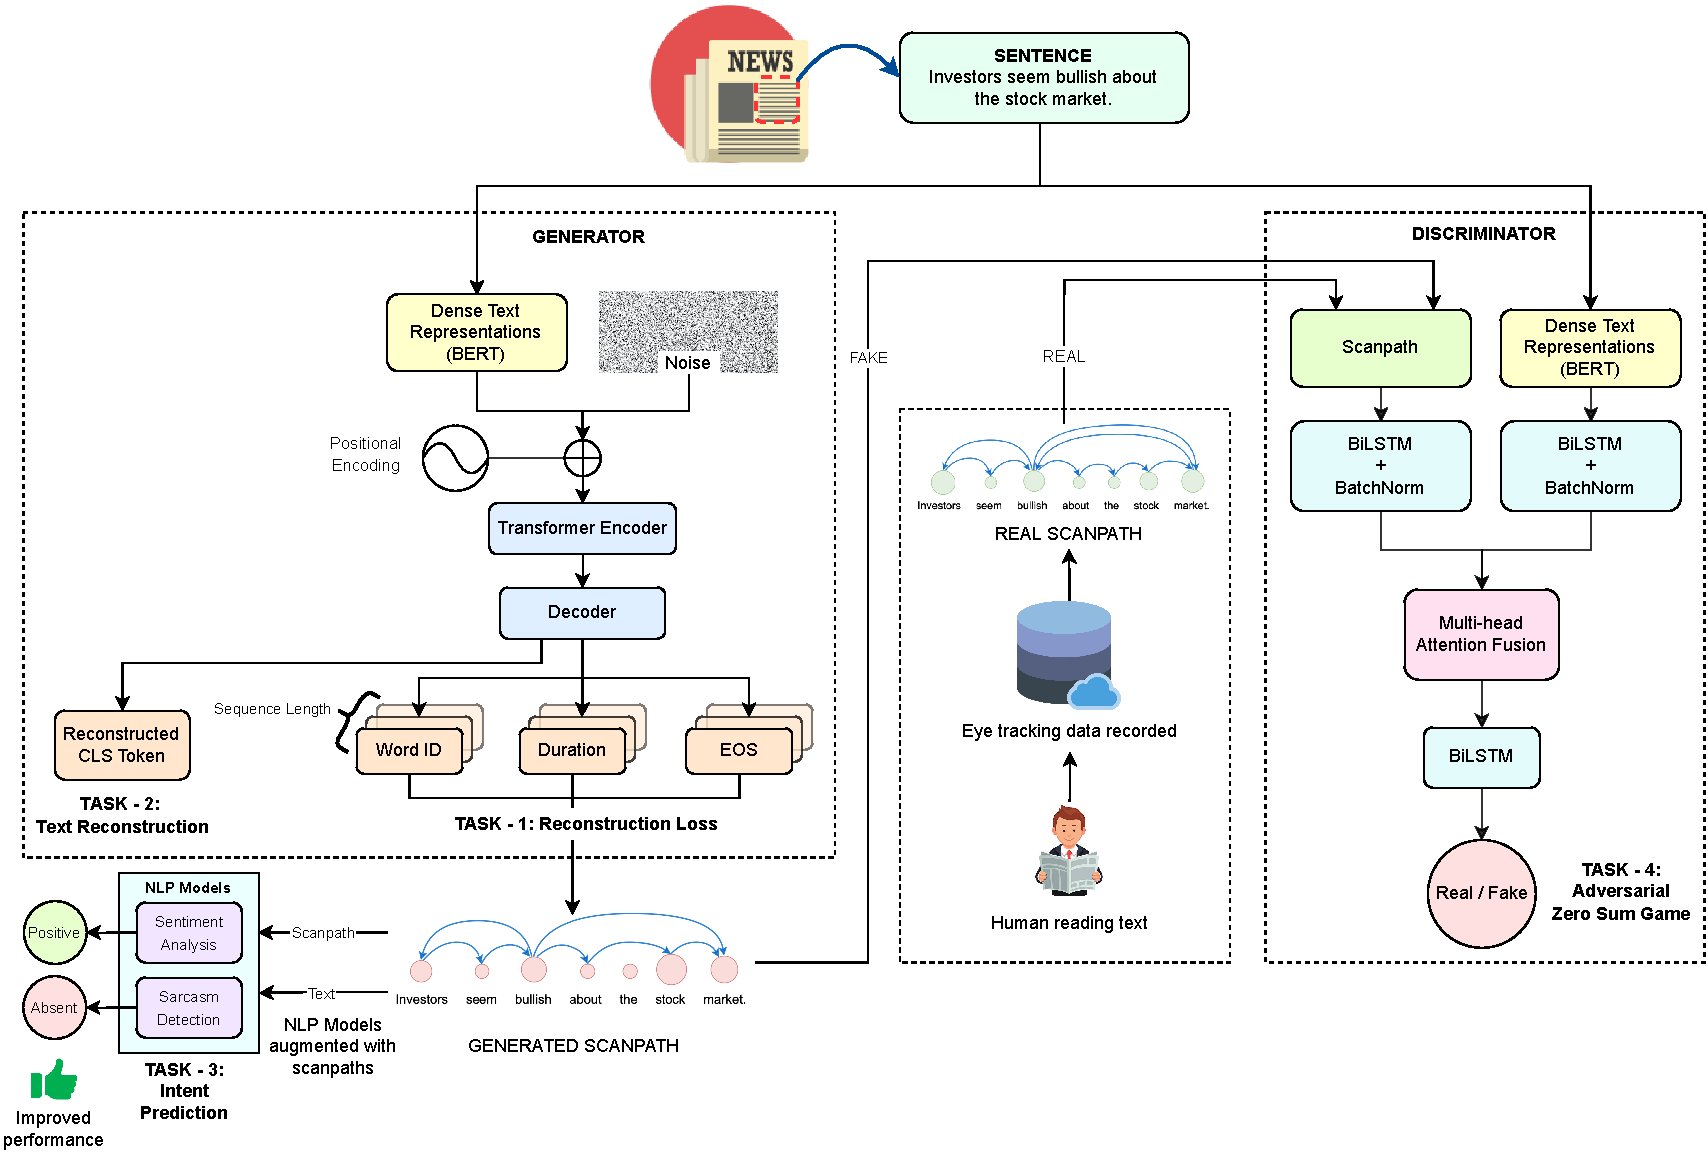
\includegraphics[width=1.2\textwidth]{images/Intent_Scanpath_Figure.pdf}
    %\vspace*{-2mm}
    \caption{The architecture of the proposed Intent-Aware \textbf{ScanTextGAN} model. The model consists of a conditional generator and a discriminator playing a zero-sum game. Two cognitively inspired losses train the generator: scanpath (Task-1) and text (Task-2) reconstruction, a loss from the downstream intent of the natural language task (Task-3), and finally, the loss from the adversarial zero-sum game (Task-4). Variations of scanpaths are generated based on the downstream natural language task.}
    \label{fig:intent-model} 
%\vspace*{-5mm}
\end{figure*}
\end{landscape}


\begin{figure*}[]
%\vspace*{-2in}
    \centering
    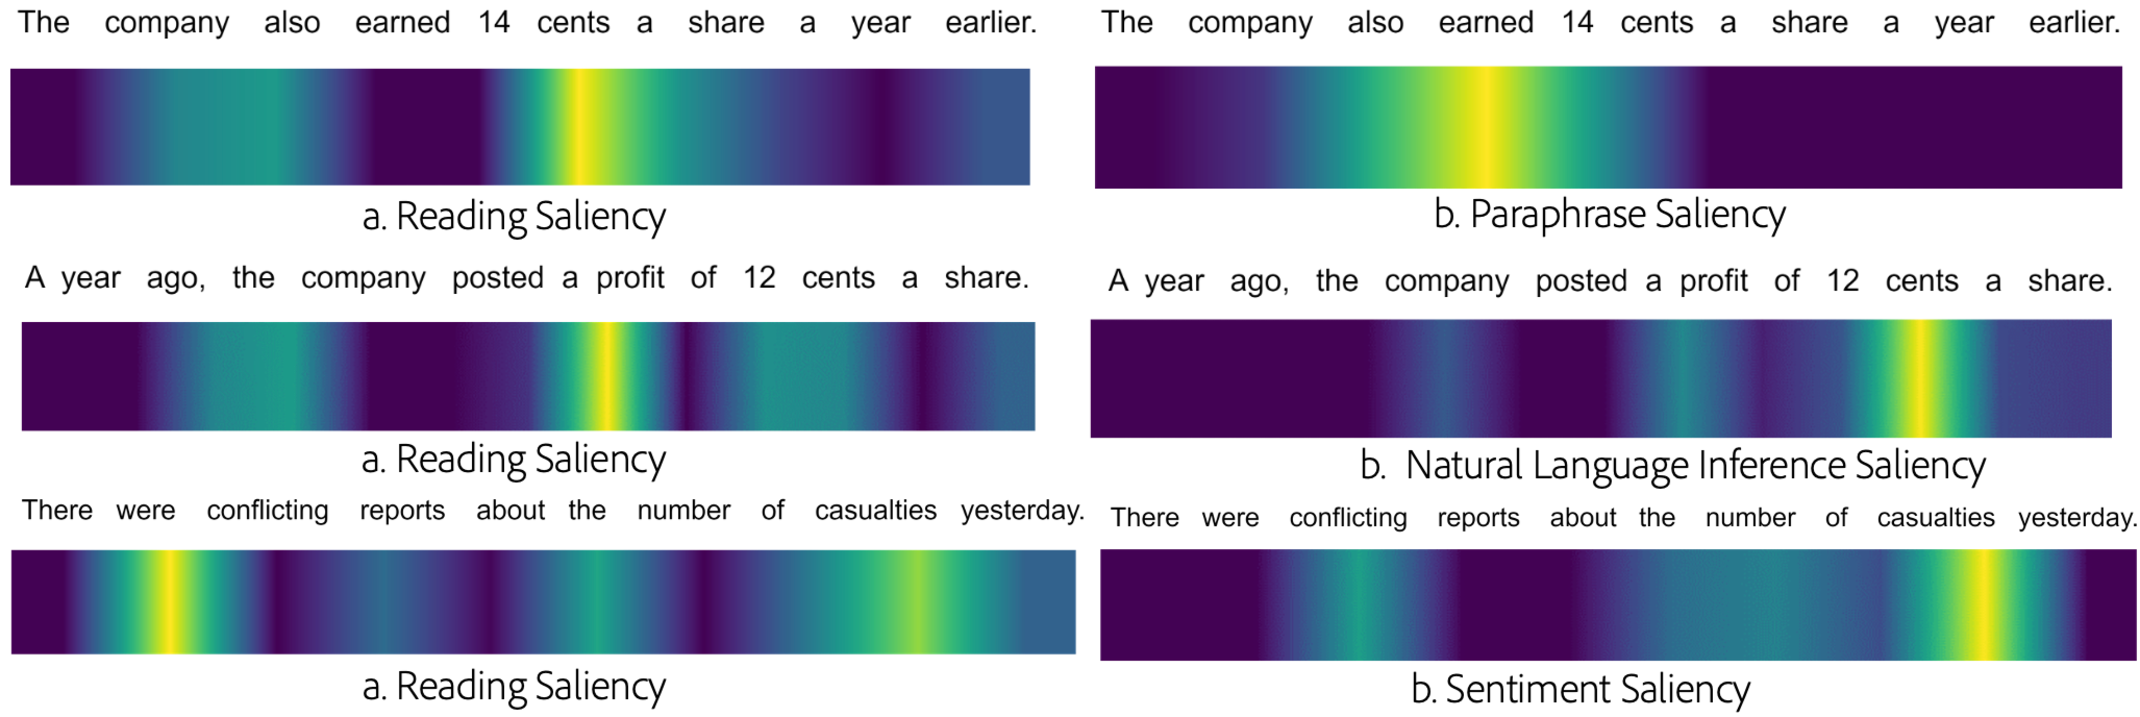
\includegraphics[width=\textwidth]{images/intent-scantextgan-saliency.pdf}
    %\vspace*{-2mm}
    \caption{Saliency samples generated by conditioning scanpath generation on different downstream natural language tasks. It can be observed that the conditioned saliency pays much more attention to words important for that downstream task.}
    \label{fig:intent-saliency-example} 
%\vspace*{-5mm}
\end{figure*}








\subsection{Limitations}
\label{Limitations}
In this work, we demonstrated artificial scanpath generation over multiple eye-tracking datasets. Further, our experiments build a link between cognitive and natural language processing and show how one can inform the other. However, the proposed method has a few limitations, which we aim to address in the future. The field needs work on bigger and more diverse eye-tracking datasets, which can enable scanpath generation over longer text sequences and can model generating scanpaths conditioned on previously read context. Besides, a better understanding of the entire scanpath generation process can help model the intra and inter-sentence scanpath generation process. The understanding would enable the integration of scanpaths to generative modeling tasks, which we intend to take up in future work. Another parallel direction is to include both explicit (like using RLHF) and implicit signals (like using cognitive signals) to better NLP tasks like language modeling.





\FloatBarrier
%%%%%%%%%%%%%%%%%%%%%%%%%%%%%%%%%%%%%
%%%%%%%%%%%%%%%%%%%%%%%%%%%%%%%%%%%%%
%%%%%%%%%%%%%%%%%%%%%%%%%%%%%%%%%%%%%
Communication is defined as ``\textit{Who} says \textit{what} to \textit{whom} with \textit{\textbf{what} effect}.'' A message from a communicator generates downstream receiver effects, also known as behavior. Receiver behavior, being a downstream effect of the message, carries rich signals about it. Even after carrying signals about the message, the behavior signal is often ignored while training vision language models. We show that training VLMs on receiver behavior can actually help improve their content-understanding abilities. We demonstrate that training VLMs to predict receiver behaviors, such as likes, comments, and replay graphs, which are available at scale, enhances the VLM's performance across a broad range of downstream content understanding tasks. We show this performance increase over 6 types of behavior, 46 different tasks covering image, video, text and audio over 26 benchmark datasets across both 0-shot and fine-tuning settings, outperforming many supervised baselines on diverse tasks ranging from emotion recognition to captioning by upto 150\%. We note that since receiver behavior, such as likes, comments, and replay graphs, is collected by default on the internet and does not need any human annotations to be useful, the performance improvement we get after training on this data is essentially free-lunch. We also release BLIFT, our Behaviour-LLaVA IFT dataset comprising of 730k images and videos with their receiver behavior collected from multiple platforms on which we train our models to achieve this.


\section{Teaching Human Behavior Improves Content Understanding Abilities Of VLMs}

Communication is defined as ``\textit{Who} says \textit{what} to \textit{whom} with \textit{\textbf{what} effect}.'' A message from a communicator generates downstream receiver effects, also known as behavior. Receiver behavior, being a downstream effect of the message, carries rich signals about it. Even after carrying signals about the message, the behavior signal is often ignored while training vision language models. We show that training VLMs on receiver behavior can actually help improve their content-understanding abilities. We demonstrate that training VLMs to predict receiver behaviors, such as likes, comments, and replay graphs, which are available at scale, enhances the VLM's performance across a broad range of downstream content understanding tasks. We show this performance increase over 6 types of behavior, 46 different tasks covering image, video, text and audio over 26 benchmark datasets across both 0-shot and fine-tuning settings, outperforming many supervised baselines on diverse tasks ranging from emotion recognition to captioning by upto 150\%. We note that since receiver behavior, such as likes, comments, and replay graphs, is collected by default on the internet and does not need any human annotations to be useful, the performance improvement we get after training on this data is essentially free-lunch. We also release BLIFT, our Behaviour-LLaVA IFT dataset comprising of 730k images and videos with their receiver behavior collected from multiple platforms on which we train our models to achieve this.


\subsection{Introduction}
Communication is defined by five factors: sender, message, channel, receiver, and behavior \cite{shannon-weaver-1949,lasswell1948structure,lasswell1971propaganda}. \citet{lasswell1948structure} encoded these five factors in the phrase, ``\textit{Who} says \textit{what} to \textit{whom} with \textit{what effect}.'' Human behavior occurs as a downstream artifact in the process of communication. Behavior is produced by the receiver as a response to the message sent by the sender. Being a downstream effect, behavior can help us infer important signals about the message itself. These signals, if properly harnessed, should be able to increase performance on the message understanding tasks popular in NLP and CV, like question answering, sentiment analysis, topic classification, \textit{etc}. Despite this, behavior data is considered noise and is ignored while training large language models \cite{biderman2022datasheet,penedo2023refinedweb} and also large vision and language models \cite{liu2023visual,zhu2023minigpt}. In this paper, we explore this line of thought more.


\begin{figure*}[h]
    \centering
        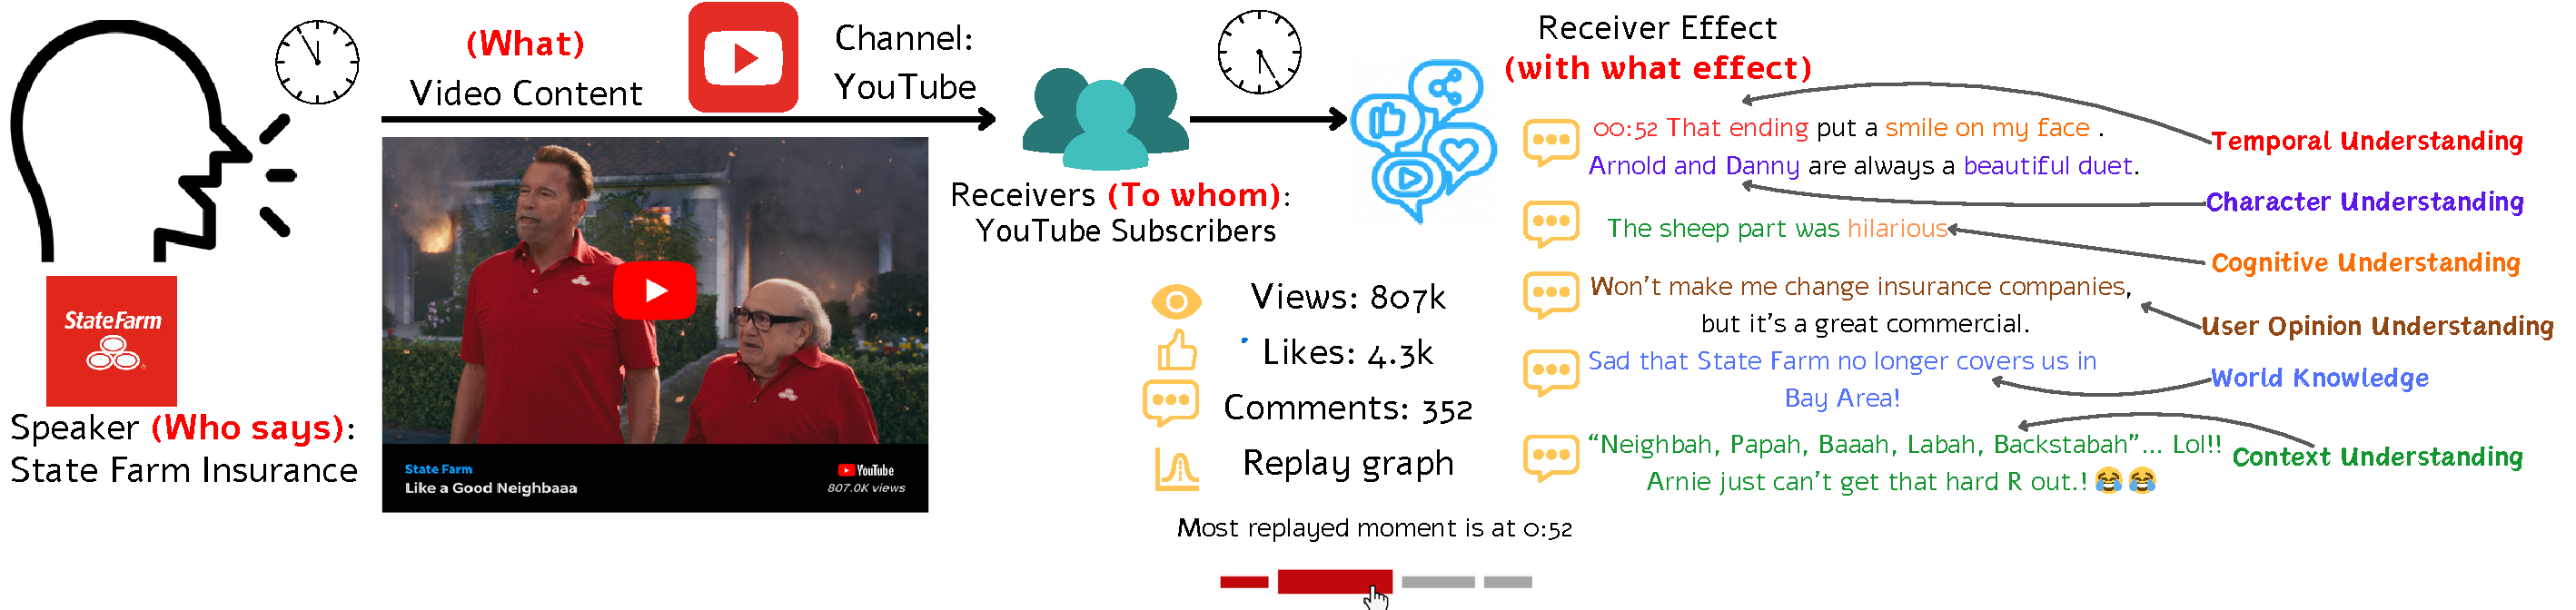
\includegraphics[width=\textwidth]{images/bllava-fig_2.pdf}
    \caption{The diagram depicts the five factors of communication in the context of an example YouTube video \url{https://www.youtube.com/watch?v=eT8hO4e2iTM} and where lies the free lunch. The receiver effect is not used while training Large Vision and Language Models. However, it contains many important signals that can help in understanding the content. The figure shows several comments containing temporal, cognitive, character, context, and user opinion information useful for understanding the video. \label{fig:synthetic-data-vs-generation-performance} }
\end{figure*}



\begin{figure*}[]

\centering
        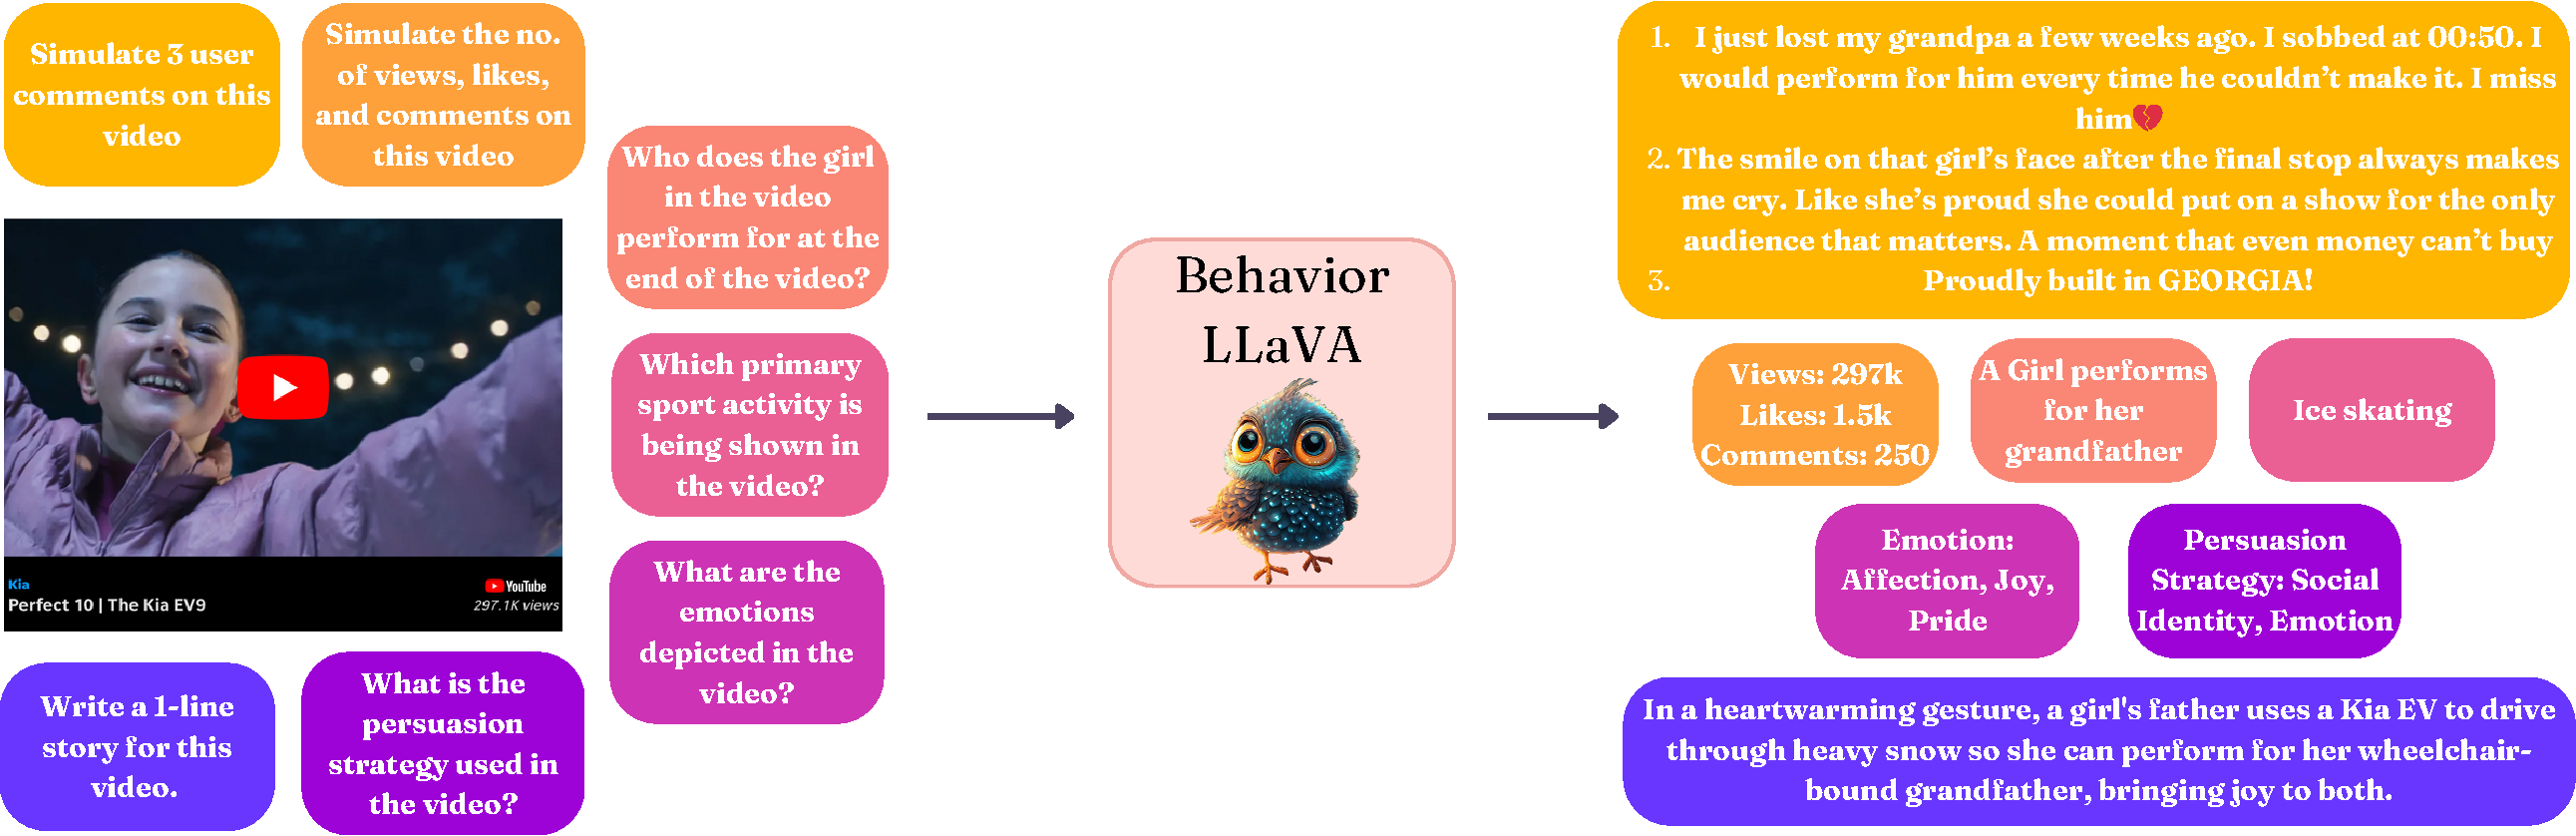
\includegraphics[width=\textwidth]{images/bllava-fig_1.pdf}
    \caption{Behavior-LLaVA is trained to answer behavioral questions like simulating user comments and likes on the video. The model, once trained, shows superior performance than LLaMA-Vid and other VLMs on content-related tasks like emotion recognition, action recognition, question answering, persuasion strategy classification, \textit{etc}. The original video was showcased in SuperBowl-2024 and is posted on YouTube on the URL \url{https://www.youtube.com/watch?v=OU7BJc96lI4}. The video is titled ``Perfect 10: The Kia big game commercial featuring the 2024 Kia EV9'' by Kia America. \label{fig:Behavior-LLaVA}}

\end{figure*}

% behavior data is available at a scale

% intersection with cognitive signals and difference wrt to it: same sample, scale
Humans produce two kinds of behavioral signals upon observing a message \cite{bertenthal1996origins,prinz1997perception}: perceptual signals and actions as behavior. Perceptual signals, like seeing, touching, and hearing, help a receiver primarily sense the world around her, ultimately guiding her actions. Actions are how a receiver acts on the outside world. 
%internal processing signals in the form of a stream of thoughts, beliefs, and affects \cite{ajzen1975bayesian,berkowitz2000causes,eagly1993psychology}, and behavior or overt actions \cite{anderson1981foundations}. Internal signals are latent and cannot be observed; only actions are observable\footnote{We also allude to the famous quip by Stanley Milgram ``Only in action can you fully realize the forces operative in social behavior'' \cite{milgram1978obedience}.} \cite{albarracin2014handbook,anderson1981foundations}. However, 
The signals produced by the human receiver upon receiving a message carry information about the message itself (Fig.~\ref{fig:synthetic-data-vs-generation-performance}). For instance, if a person's heartbeat rises upon watching a movie scene, it can help us infer that perhaps the scene was an exciting scene \cite{dzedzickis2020human}. Similarly, regressing while reading is indicative of important or confusing phrases \cite{bicknell2011readers}. In these cases, perception behavior helps us derive inferences about content. In a similar vein, the actions a person performs after watching a movie, such as comments and likes, carry signals about the movie (Fig.~\ref{fig:synthetic-data-vs-generation-performance}, \ref{fig:Behavior-LLaVA}). 

Expanding on these ideas, prior literature has shown that harnessing perceptual signals, like eye movements, saliency, keystrokes, mouse movements, and FMRI, by modeling them together with content understanding tasks can improve both NLP and CV tasks. For instance, integration with perception signals causes performance improvement in tasks like visual and natural language question answering \cite{patro2018differential,khurana-etal-2023-synthesizing,sood2020improving}, text and image sentiment analysis \cite{khurana-etal-2023-synthesizing,barrett-etal-2018-sequence,fan2018emotional}, natural language inference \cite{khurana-etal-2023-synthesizing}, part-of-speech identification \cite{barrett-etal-2016-weakly,barrett-etal-2016-cross}, named entity recognition \cite{hollenstein2019advancing,NoraNEREyeTracking}, syntactic parsing \cite{plank2016keystroke}, image captioning \cite{cornia2018paying}, and visual object detection \cite{wang2018salient,kruthiventi2016saliency}. % Similarly, digital analytics like comments and likes carry various types of information like. These 



While the initial studies show that perceptual signals have much promise for improving downstream content understanding, they have a few significant issues due to which integrating human perception has not seen wide adoption in training LLMs. These perceptual signals can only be collected in lab settings requiring specialized lab equipment and are thus expensive to collect and thus are also limited in number. For example, the largest datasets containing the human processing signals are SALICON \cite{jiang2015salicon} and \citet{cheng2014global} for visual saliency (10k images each), CELER \cite{berzak2022celer} and Dundee corpus \cite{kennedy2013frequency}  containing eye movements over 28k sentences and 20 news articles respectively, and \citet{dhakal2018observations} containing keystroke patterns over 1.5k sentences. Clearly, these datasets, while making important contributions, do not scale to the level at which today's large language models are trained (trillions of natural language and image tokens). %Further, being restricted to lab settings also limits the types of demographics reachable by the lab, thus limiting their representativeness of human diversity. Lab settings also lead to people changing their behavior in response to their awareness of being observed, an effect commonly called the Hawthorne effect \cite{mccarney2007hawthorne,roethlisberger2003management,malavolta2022awareness}. 


On the other hand, actions (the other type of behavioral signals produced by a human receiver) are collected at a large scale in the form of digital analytics. Examples of this kind of data are likes, views, shares, comments, and purchase histories on images, tweets, videos, webpages, and other kinds of media. Action data has a much broader representation than is possible in lab settings, is available on more diverse content, and is much cheaper to collect than using specialized lab equipment. At the same time, actions have not been much investigated in the literature for their potential to improve downstream content understanding. %Further, they are much more noisier than perceptual signals collected in the lab, owing to their collection in real-world settings. 
%Due to their nature, perceptual signals are primarily observed with lab equipment, like eye trackers, MRI, and heart monitors. On the other hand, behavior or overt actions are recorded in the real world in the form of big data or digital analytics.  These are widely (and cheaply) collected on a large scale. 


Therefore, in this paper, we make initial efforts to collect and understand digital analytics at scale with the aim of integrating them with VLMs to improve their downstream content understanding capabilities. We introduce methods for filtering and cleaning behavioral data and then propose tasks for large language and vision models, leading to improvements in language and visual content understanding tasks. For this, we look to Reddit and YouTube as two major sources of visual content and human behavior in the form of viewer comments, likes, replay graphs, and upvotes. From Reddit, we collect 5 million images and videos along with their upvotes and top-upvoted comments from two major subreddits (r/pics and r/videos). Similarly, from YouTube, we collect 2.2 million videos from 30000 channels along with their likes, views, replay graphs, and top user comments. After extensive filtering and cleaning, we are left with 730k samples of videos and images across the two platforms which we use for the next steps. 





After collecting user behavior over image and video content, we design tasks to teach large vision and language models (VLMs) to simulate user behavior. For this, we use an instruction fine-tuning format. Given a video or an image and the other metadata like time of post and channel, we ask the model to simulate user behavior of likes and comments. See Fig~\ref{fig:Behavior-LLaVA}, Listing~\ref{lst:blift-template} for examples. We choose LLaMA-Vid \cite{li2023llamavid} as our base model to teach it the user behavior. We call the resultant model Behavior-LLaVA (Large Language and Vision Assistant) \cite{liu2023visual}. We test Behavior-LLaVA on a diverse variety of tasks, evaluating its capabilities on image, video, text, and audio understanding tasks. We compare Behavior-LLaVA against its base model, LLaMA-Vid, and other supervised baselines. Further, to show the impact of behavior, we train another version of LLaMA-Vid, where we train it on the same set of videos and images as Behavior-LLaVA but do not include behavior information. We call this model Ad-LLaVA.

% XXX: gel it with previous paragraph
%Note that all the vision language models \cite{liu2023visual,zhu2023minigpt,huang2024language,li2023blip2,li2023llamavid} are trained on image-text instructions where text is some kind of human annotations \cite{lin2014microsoft,sharma2018conceptual} or generated by stronger LLMs like GPT-4. 

%Both these options require a significant amount of money. It is noteworthy that our model does not add any extra annotation or API cost to generate data. Rather, we rely on sampling data from digital analytics databases, which are anyway being collected for various reasons.%, and use them to improve VLM capabilities. Therefore, any potential improvements brought by integrating action data with VLMs do not require a significant capital investment.


\begin{figure}
    \centering
 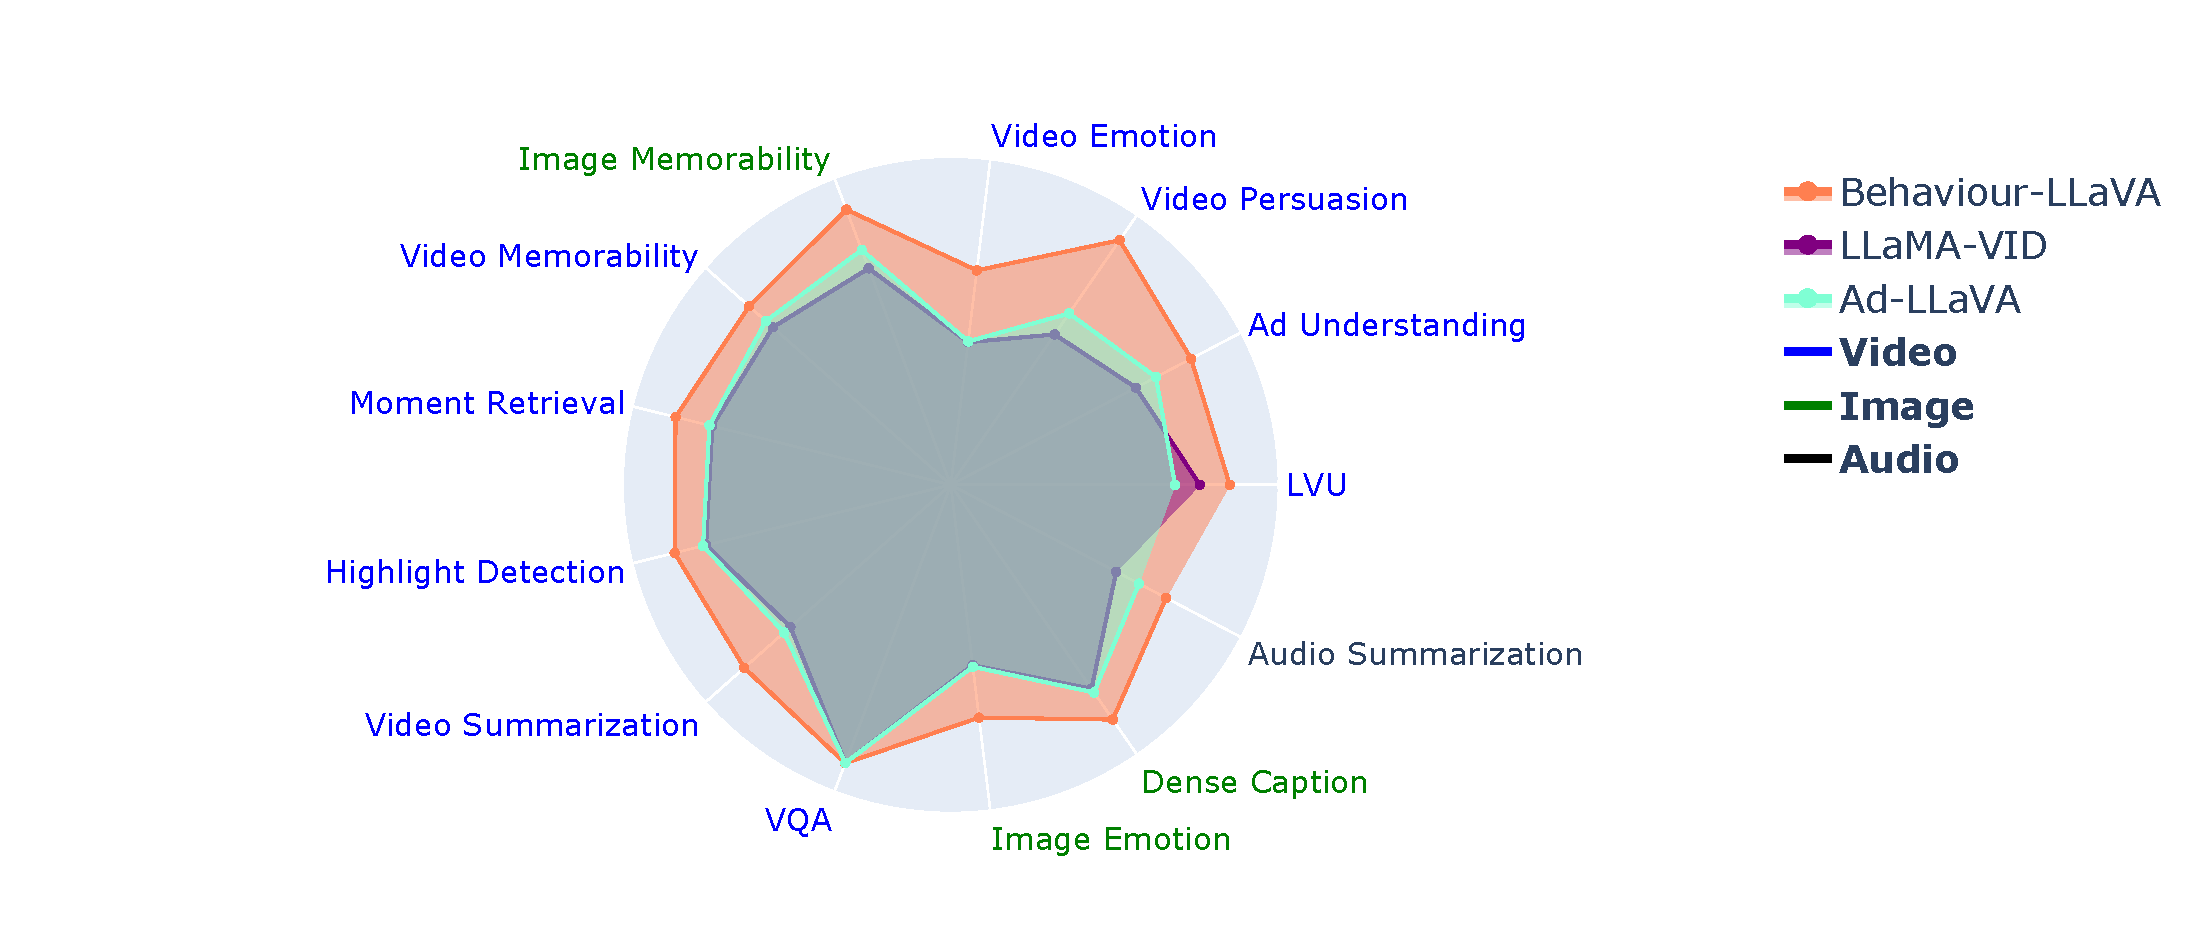
\includegraphics[width=0.9\linewidth]{images/radar_chart.pdf}
\vspace*{-10pt}    
\caption{Behaviour-LLava achieves much higher zero-shot performance compared to Ad-LLaVA and the base model LLaMA-VID across a diverse suite of image, video, and audio benchmarks.}
    \label{fig:star-graph}

\end{figure}

We make the following contributions with this work:\vspace{0.1cm}\\
1)~\textbf{Behavior-LLaVA Instruction Fine-Tuning:} We explore the idea of learning human behavior, resulting in better content understanding. We test this for action-level behavior data such as receiver comments, likes, and replay graphs. We collect a dataset called \textbf{BLIFT}, consisting of 400k images and 330k videos, along with their receiver behavior. Then, LLaMA-Vid is trained for the task of predicting receiver comments and upvotes given a media (a video or an image) (Listing~\ref{lst:blift-template}). We show that using this simple task formulation over behavioral data collected in the wild, results in performance improvement over a hierarchy of tasks. We get improvements over the base LLaMA-Vid across 46 tasks over 26 benchmark datasets in both zero-shot and fine-tuned settings. We show this over low-level content understanding tasks like object and activity recognition and also over high-level tasks like topic and emotion detection. 
%Further, interestingly, none of the tasks tested show a significant decrease in performance by training LLaMA-Vid on this additional task. 
Through this, we propose a scalable approach to increase the content understanding abilities of VLMs, requiring minimal cost and no architectural changes. 


2)~\textbf{AdLLaVA: Disentangling the effect of content and behaviour:} To disentangle the effect of training LLaMA-Vid on additional image and video data from the effect of training on behavior data, we train LLaMA-Vid on BLIFT's videos and images without including behavior. We call this model Ad-LLaVA. We show that Ad-LLaVA shows equivalent performance as its base model LLaVA-Vid; however, Behavior-LLaVA  performs better than both Ad-LLaVA and LLaMA-Vid, thus highlighting the importance of behavior data and instruction fine-tuning on behavior data.

%3)~Further, to show the generalization of the hypothesis of modeling human behavior resulting in better content understanding, we show results on five human behaviors: likes, comments, replay graphs, video highlights, and memorability. 

3)~\textbf{Perception vs Action:}We also show an ablation of Behavior-LLaVA across different kinds of behavior. We try out the perception behavior of saliency prediction over images and five types of action-level behavior over images and videos. We find that perception-level behavior does not result in significant performance improvements; however, action-level behavior shows improvements across all the tasks. We posit that one reason for this could be due to the scale for which action-level data is available (Table~\ref{tab:salicon-ablation}). While perception behavior is mostly collected in lab settings, action-level behavior data is diverse, can be collected in a scalable manner automatically and cheaply.




%3)~Finally, we release the first large-scale video emotion, persuasion strategy, and topic dataset over 100k videos. We label the videos in the dataset automatically using Behavior-LLaVA. We show that learning a model on this automatically labeled dataset results in performance on the existing video and image benchmarks (Table~\ref{}) in 0-shot settings.

%Effect (or behavior) over a content can also enable us to understand about the content, the communicator, the receiver, or the time. Therefore, efforts have also been made to extract information about the content itself from the behavior it generates. For instance, using keystroke movements \cite{plank2016keystroke} and eye movements to improve natural language processing \cite{klerke2016improving,khurana-etal-2023-synthesizing}. Similarly, the fields of human alignment and reinforcement learning with human feedback (RLHF) try to use human behavioral signals of likes, upvotes, downloads, and annotations of a response's helpfulness to improve content generation - both text \cite{kreutzer2018can,stiennon2020learning,ziegler2019fine,nakano2021webgpt,si2023long} and images \cite{lee2023aligning,pressman2023simulacra,wu2023better,khurana-etal-2023-synthesizing}.







\begin{comment}
    \begin{enumerate}
        \item Hierarchy of tasks (object detection, QA, emotion and persuasion) across hierarchy of behaviors (saliency (perception stage) vs likes (reaction stage; with a lower cognitive effort) vs comments (reaction stage; with a higher cognitive effort))
        \item Scalable for approach of learning cognitive labels (CS) using receiver behavior (BS).
            \begin{enumerate}
                \item Emotion, Memorability, Persuasion, Atypicality, LVU, HVU (0-shot vs sft) | (sota and same model 0-shot/sft without comments) | (GPT)
                \item Train on Likes vs Comments (Ablation)
                %(Likes + comments)
            \end{enumerate}
        \item Scalable approach of 0-shot transferring affective (emotion, persuasion, Topic-Action-Reason) labels across Modalities
        \item SOTA Image and Video Emotion, Persuasion, TAR Model
        \item First large-scale video emotion, persuasion, topic, action-reason, atypicality datasets (160k).
            \begin{enumerate}
                \item Human Study on video affect dataset showing \% agreements with the pseudo-labeled datasets
            \end{enumerate}
        %\item We show downstream improvement in behaviour understanding by including comments and affective labels in training data.
    \end{enumerate}
    
    
    %``\textit{The question is not whether intelligent machines can have any emotions, but whether machines can be intelligent without emotions.}'' - Marvin Minsky, Turing award winner. 
    
    
    Contributions:
    %1. VideoAffect, First large-scale video emotion dataset.\\
    %2. Advancing the field of domain transfer in affective computing, we show that language can act as a gel between the image and the video modalities, allowing the transfer of a model trained on image emotions to work on emotion tagging for videos. \\
    %3. Affective labels for videos, other than being useful on their own, can also improve the performance in several downstream applications. To show the utility of VideoAffect, we show that emotion labels learned using VideoAffect improve performance on three real-world applications: behavior simulation, memorability prediction, and persuasion strategy classification.
    
    
    
    Domain transfer in affective computing - 
    
    Trends in affect datasets:
    1. Web scale - 
    
    downstream applications of affective computing - education \cite{yadegaridehkordi2019affective}, healthcare \cite{yannakakis2018enhancing}, advertising \cite{shukla2020recognition,sanchez2020opinion}, social media \cite{}
    
    
    \begin{enumerate}
        \item Adding cognitive tags helps on downstream performance (YT likes, Image and Twitter Likes, Image and Video Reddit Upvotes, Image and Video Memorability, Image and Video Persuasion Strategies, LVU/HVU tasks.
    \end{enumerate}
    
\end{comment}

\begin{comment}
    
    \section*{TODO}
    Add verbalization for evaluation benchmarks (Verbalization done, Story is left)
    
    Options rather than predicting labels in Kovashka Action Reason
    
    \begin{enumerate}
    \item Request eMOTIONS (Not available)
    \item Joint Training
    
        \item (r/pics r/videos Brands80k) Media+Verbalization -> Comments
        \item EmotionNet -> media + verbalization -> Image Emotions
        \item eMOTIONS -> verbalization + media -> emotions 
    \item Image Emotion Model EmotionNet -> media + verbalization -> Image Emotions. Do comments improve image emotion modelling
    \item How Do Video Comments scale for video emotions (0k, 5k, 50k, 160k)
    \item Did video emotion help?
    \item Video Emotion Benchmarks
    \item Behavior Benchmarks
    \item Ablate on Verbalization
    \item Video Dataset -> small model
    
        \item 0-shot LLaVA on benchmarks
        \item Fine-Tune +0 shot modality Transfer
        \item Create Labellled dataset (BLINK)
        \item FineTune on BLINK and test on Modalities
            \begin{enumerate}
                \item reddit images + comments -> videos/gifs + comments(emotion)
                \item adsofworld videos + story -> images (persuasion) [VideoLLM dataset (Video Persuasion)]
            \end{enumerate}
        \item BLINK Finetuned model on downstream tasks (tags or finetuned)
            \item Kovashka tasks
            \item Twitter Likes
            \item Memorability
            \item HVU
        \item Get YouTube Top Links for videos without comments @harini
        
    \end{enumerate}
    

\end{comment}


    % \item Image Emotion SOTA model using LLaVA + Verbalization on hierarchical emotions. (Derived from \cite{})
    % \begin{enumerate}
    %     \item Finetune LLaVA1.5 + verbalization on Stock Emotions dataset, and compare with existing.
    %     \item Use current hierarchial mapping for combining different datasets (Kovashka/WebEmo)
    % \end{enumerate}
    % \item Video Emotion Model by fine-tuning Image Emotions
    % \begin{enumerate}
    %     \item Mean Pool VIT embeddings, and video verbalization for finetuning on small dataset (2k videos) \cite{}
    % \end{enumerate}
    % \item Semi-supervised data collection and Pseudo Labeling model
    % \begin{enumerate}
    %     \item For Pairs of (Title, Comments, Image, Caption/Alt-Text from r/pics) get 0-shot Emotions
    %     \item Train BERT for (Title, Comments, Caption)->Emotions
    %     \item Make Pseudo-labels \cite{} for Video using (Title, Comments, Caption) on r/videos
    %     \item Filter Pseudo-labels \cite{}
    % \end{enumerate}
    % \item SSL for Image Emotion and Video Emotion
    % \begin{enumerate}
    %     \item Show improvement using SSL in terms of \% Supervised data seen and Accuracy on Images/Videos
    % \end{enumerate}
    % \item Evaluating the Language Gel by Calculating attention across 
    % scenes
    %     \begin{enumerate}
    %         \item Show with / without verbalization learning curves
    %         \item Show attention map while predicting an emotion on scene description to show qualitatively how language gels image-video
    %     \end{enumerate}

    % \item To show performance improvements on the following downstream applications:
    %     \begin{enumerate}
    %         \item Behavior simulation on twitter like prediction or Reddit upvotes
            
    %         \item Video emotions prediction on existing datasets - VideoEmotion-8 (\url{https://cdn.aaai.org/ojs/8724/8724-13-12252-1-2-20201228.pdf}), Kovashka Ads, Ekman-6 (\url{https://arxiv.org/abs/1908.05913}), CAER (\url{https://ieeexplore.ieee.org/document/7723914/})

    %         \item Persuasion strategy prediction on videos
            
    %     \end{enumerate}
    % \item Images (Images First)
    %     \begin{enumerate}
    %         \item Train Set: Emotion-Net (Verbalized)
    %         \item Webemo + Emotion6 + Kovashka [TRAIN-SET](Not Verbalized)
    %         \item Adsofworld (Verbalized)
    %         \item Reddit r\\images (verbalized)
    %     \end{enumerate}
    % \item Videos
    %     \begin{enumerate}
    %         \item Kovashka (Verbalized)
    %         \item Adsofworld (Verbalized mostly)
    %         \item  r\\videos (Not verbalized) @ tarun
    %         \item  r\\gifs (Not verbalized) frame extraction
    %         \item YouTube (Not verbalized) @tarun
    %         \item CAER [TEST-SET] (Not verbalized) 
    %     \end{enumerate}






%%%%%%%%%%%%%%%%%%%%%%%%%%%%%%%%%%%%%%%%%%%%%%%%%%%%%%%%
%%%%%%%%%%%%%%%%%%%%%%%%%%%%%%%%%%%%%%%%%%%%%%%%%%%%%%%%
\subsection{Methodology}
\label{sec:methodology}
In this section, we introduce our approach to train Behavior-LLaVA. Since no publicly available corpus consists of behavior together with image and video content, we first introduce our instruction fine-tuning dataset, ``Behavior-LLaVA Instruction Fine-Tuning dataset'' (BLIFT). Next, we introduce our methodology to train Behavior-LLaVA. Finally, we report the results of testing Behavior-LLaVA's capabilities on a hierarchy of tasks. The tasks cover low-level media understanding tasks like object and activity detection, high-level media understanding tasks like emotion, topic, and persuasion strategy classification. 


\subsubsection{BLIFT Dataset}
Given the abundance of media and behavioral data and its accessibility, our data collection relies on two primary sources: Reddit and YouTube. These platforms share similarities in terms of hosting media content (images and videos) and providing user engagement metrics in the form of Reddit upvotes and comments, and YouTube likes, views, comments, and replay graphs. Here, we delineate the process involved in constructing the instruction fine-tuning dataset, which we term as the Behavior-LLaVA Instruction Fine-Tuning (BLIFT) dataset.



\paragraph{Data from Reddit} To collect a substantial corpus of diverse images and videos, we targeted at two specific subreddits, namely r/pics and r/videos. Established over 15 years ago, these subreddits had a user base exceeding 20 million during the data collection period, with an average of over 5,000 online users concurrently. Notably, due to stringent content moderation guidelines \cite{reddit_content_policy,reddit_pics_rule8,reddit_pics_wiki_index,reddit_videos_rules} and the exclusive focus of these subreddits on media content, they offer a rich variety of content devoid of thematic biases. Our data collection spans until January 2022, during which the activity on these subreddits witnessed a notable decline following several policy adjustments and user protests \cite{guardian_reddit_protest,economist_reddit_protest}.


% r/pics added the rule for adding pics without digital/overlay text only in Feb 2015. Therefore we discard all further analysis before that. These count to a total of 3.1M images and 2M videos. Both of these subreddits ranked under 20 consistently since 2017, reached 20M members and 1000 comments per day consistently from Jan 2018 onwards, therefore we consider posts from Jan 2018. These total to 1.4M images and 1.1M videos 

To ensure data quality and relevance, we executed a series of filtering steps on the posts and comments from these subreddits. Initially, we excluded posts predating February 2015 from r/pics, coinciding with the implementation of a rule requiring images without digital/overlay text \cite{reddit_pics_rule8,reddit_pics_wiki_index}. This filtering step resulted in the exclusion of 3.1 million images and 2 million videos. Subsequently, considering the sustained popularity of both subreddits, with rankings within the top 20 since 2017 and consistent membership exceeding 20 million, we confined our dataset to posts from January 2018 onwards. This selection process yielded 1.4 million images and 1.1 million videos.

Further refinement of the dataset involved removing posts and comments marked as NSFW, BOT-generated, or [deleted], along with eliminating duplicate images and videos. This curation step reduced the dataset to 876,000 images and 983,000 videos. To address redundancy in comments, we excluded those comprising fewer than three words and employed TF-IDF-based deduplication with a similarity threshold of 0.6, determined through manual observations.

Following these steps, posts with fewer than two comments were filtered out, resulting in a dataset comprising 631,000 images and 397,000 videos. Additionally, videos exceeding a duration of 500 seconds were omitted, leaving 221,000 videos for analysis. Notably, images not directly hosted on Reddit were excluded due to scraping and copyright limitations. Similarly, for r/videos, only videos hosted on YouTube were considered. It is pertinent to mention that approximately 51\% of YouTube videos collected during this period were either made private/unlisted or removed, resulting in 400,000 images and 80,000 videos, accompanied by 1.5 million and 312,000 comments, respectively. These comprehensive filtering steps ensured the construction of a diverse and relevant dataset for fine-tuning instruction-based models. 

% write the inference and elaborate more 


\begin{comment}
    \subsubsection{Reddit}
    
    For getting a large corpus of images and videos we consider two subreddits, r/pics and r/videos. These subreddits were created at least 15 years ago and had more than 20 million users during the crawl period. Each of these had an average of 5k online users during the crawl period. We only consider data till Jan 2022; due to multiple policy changes and Reddit user's protests the activity on these three subreddits drastically reduced as seen in. Due to the content moderation rules and the topic of these subreddits being solely media, we get the most diverse content from these subreddits which are void of topic related artifacts.
    
    Following are the steps to filter the posts and comments for creating the dataset.
    
    \begin{enumerate}
        \item We remove all the NSFW,BOT, or [deleted] marked posts and comments. Further we remove all the repeated images and videos and combine their comments. These reduce to 876k images and 983k videos.
        \item We consider comments with atleast three words, to remove duplicate comments we deduplicate using TF-IDF on a similarity score of 0.6 which we decided by manual observations.
        \item After this, we remove all the posts with less than 2 comments. We are left with 631k images and 397k videos.
        \item We remove all videos with a duration greater than 500 seconds. We are left with 221k videos.
        \item We don't consider images that were not hosted on reddit due to their scraping and copyright limitations. Similarly for r/videos we only consider videos hosted on youtube. Further around 51\% of Youtube videos at the time of collection were made private/unlisted or removed. This totals to 400k images and 80k videos, with 1.5M and 312k comments respectively.
    \end{enumerate}
    
\end{comment}


\begin{figure}[!h]

    \begin{minipage}[c]{0.26\textwidth}
        \centering
        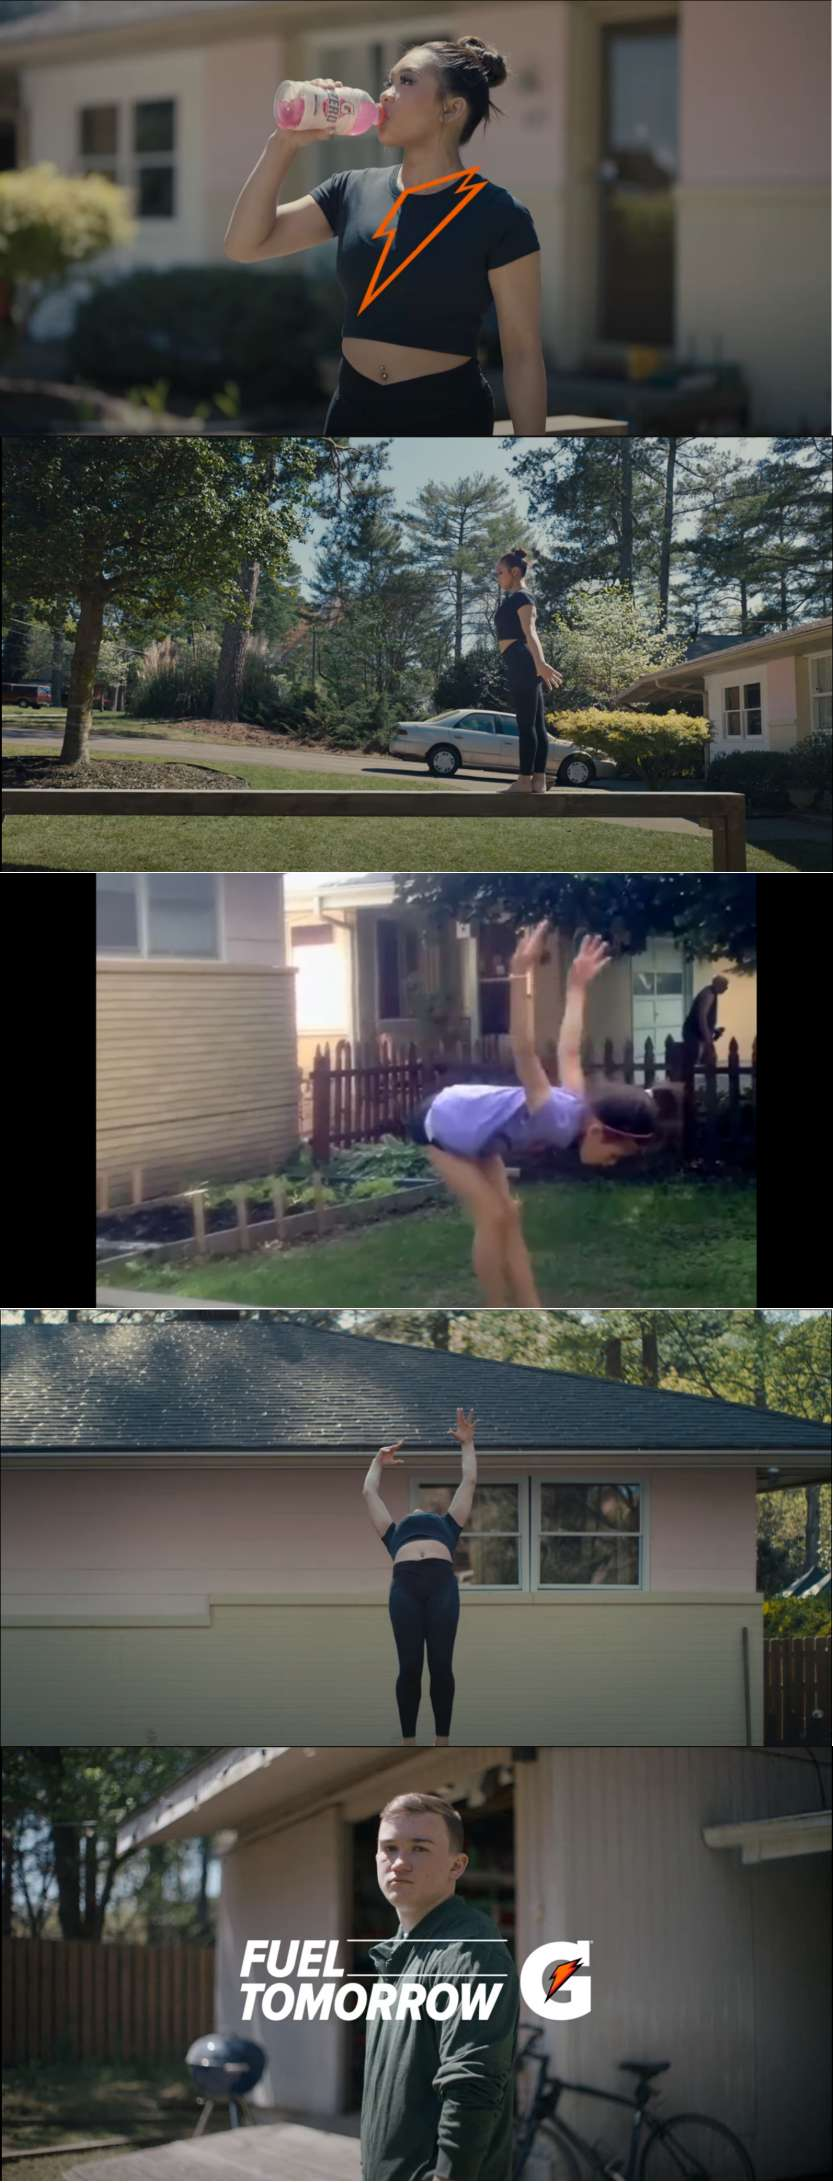
\includegraphics[width=\textwidth]{images/listing-video_compressed.pdf}
    \end{minipage}
    \hfill
    \begin{minipage}[c]{0.71\textwidth}
        \small
        \centering
        \begin{lstlisting}[caption={\scriptsize Behavior Instruction fine-tuning template for the video: \url{https://www.youtube.com/watch?v=BKPQkjRF4yY}}, 
                            frame=single, breaklines=true, basicstyle=\tiny\ttfamily, escapeinside={(*@}{@*)}, label={lst:blift-template}]
<SYSTEM>You are an AI visual assistant. You are given a detailed description of a media, followed by the actual media. Answer all questions as if you are seeing the media.</SYSTEM>

<USER>
The video advertisement is titled "Gatorade | Make Your Own Footsteps with Suni Lee" for the brand Gatorade. The audio in the ad says "[ASR HERE ...]". Analyze this video deeply, then write scene by scene description of the video and answer the following questions. What percentage of viewers would like this video, and what would be the top-5 popular comments on this video? What would the replay graph values for each scene be?
<video>...</video>
</USER>

<ASSISTANT> 
The scene-by-scene descriptions are: 

Scene 1: The scene shows a woman looking off into the distance with an orange line going around the outside of the screen. The foreground colors of the scene are black, mud green, gray, dark gray, and the background colors are dark brown, black, dark gray. The dominant tone of the scene is neutral. This scene is categorized by the tags: cosmetic, eyebrow, face, girl, ponytail, stand, string, woman.
Scene 2: The scene shows a woman balancing on a skateboard in a yard. The foreground colors of the scene are black, mud green, dark gray, olive, and the background colors are black, dark gray, gray, dark brown.The dominant tone of the scene is neutral. This scene is categorized by the tags: athletic, balance, beam, car, girl, house exterior, hurdle, jog, legging, plank, rail, seesaw, woman, yard.
Scene 3: The scene shows a girl jumping over a wooden ramp in the backyard. The foreground colors of the scene are black, dark gray, gray, dark blue, and the background colors are dark brown, dark blue, purple, dark pink, brown. 
...

>>> BEHAVIOR <<<

The video will be liked by 2.0% of viewers, and the popular comments could be:
1. "Wow. Love it. She's such an inspiration to the next generation as well as everyone."
2. "Inspiring and great story behind this commercial. Builds meaning and purpose in the hearts and minds of youth. It's been a while since good, meaningful ads have been made."
3. "She's an inspiration to the world. Thanks to her,my niece is learning gymnastics. Hopefully someday, she is an inspiration to others as Suni is an to everyone"
4. "Chills watching this. Such an inspiration."
5. "Yooooo, this is straight up!"

The replay values for each scene would be:
Scene 1: 0.06
Scene 2: 0.23
Scene 3: 0.38
...
</ASSISTANT>

\end{lstlisting}
    \end{minipage}
    \caption{Behavior Instruction fine-tuning template for the video: \url{https://www.youtube.com/watch?v=BKPQkjRF4yY}}
    \label{fig:listing-video-1}
\end{figure}

\paragraph{Data from YouTube} Our data collection from YouTube begins with querying Wikidata \cite{10.1145/2629489} for YouTube IDs to compile a list of channels. Wikidata, derived from Wikipedia, provides a curated selection of renowned channels, automatically filtering out noisy videos commonly found in datasets collected from diverse sources like user-generated videos. This initial step yielded a dataset of 2.2 million videos spanning the period from 2018 to 2023, sourced from approximately 6,000 channels collected from Wikidata.

To refine the dataset, manual filtering was employed to exclude certain categories deemed less relevant for our purposes. These categories included music and songs, gaming content, non-English videos, sports commentary, anime, memes, channels with disabled comments sections, and news-related content. Furthermore, and only videos with a substantial viewership, defined as greater than 10,000 views, were retained. We observed that these videos usually have less noisy comments and likes.

Subsequently, the top comments from each video, as ordered by YouTube (i.e., the most liked comments), were selected for inclusion in the dataset. To address redundancy in comments, a TF-IDF filter was applied with a threshold of 0.7, which proved effective in removing duplicate comments prevalent in YouTube data.

Comments were further filtered to include only those with a minimum of four words and a maximum of 100 words, ensuring a balance between relevance and conciseness. Additionally, to mitigate the presence of NSFW content, a vocabulary specific to NSFW terms \cite{ldnoobw} was employed to filter out inappropriate posts. On average, we finally get 3.1 comments per video, providing a substantial corpus of user-generated content for analysis. After applying these filtering steps, the dataset was reduced to 250,000 videos, ensuring a curated and relevant collection for subsequent analysis and model training.





\begin{figure}
    \centering
    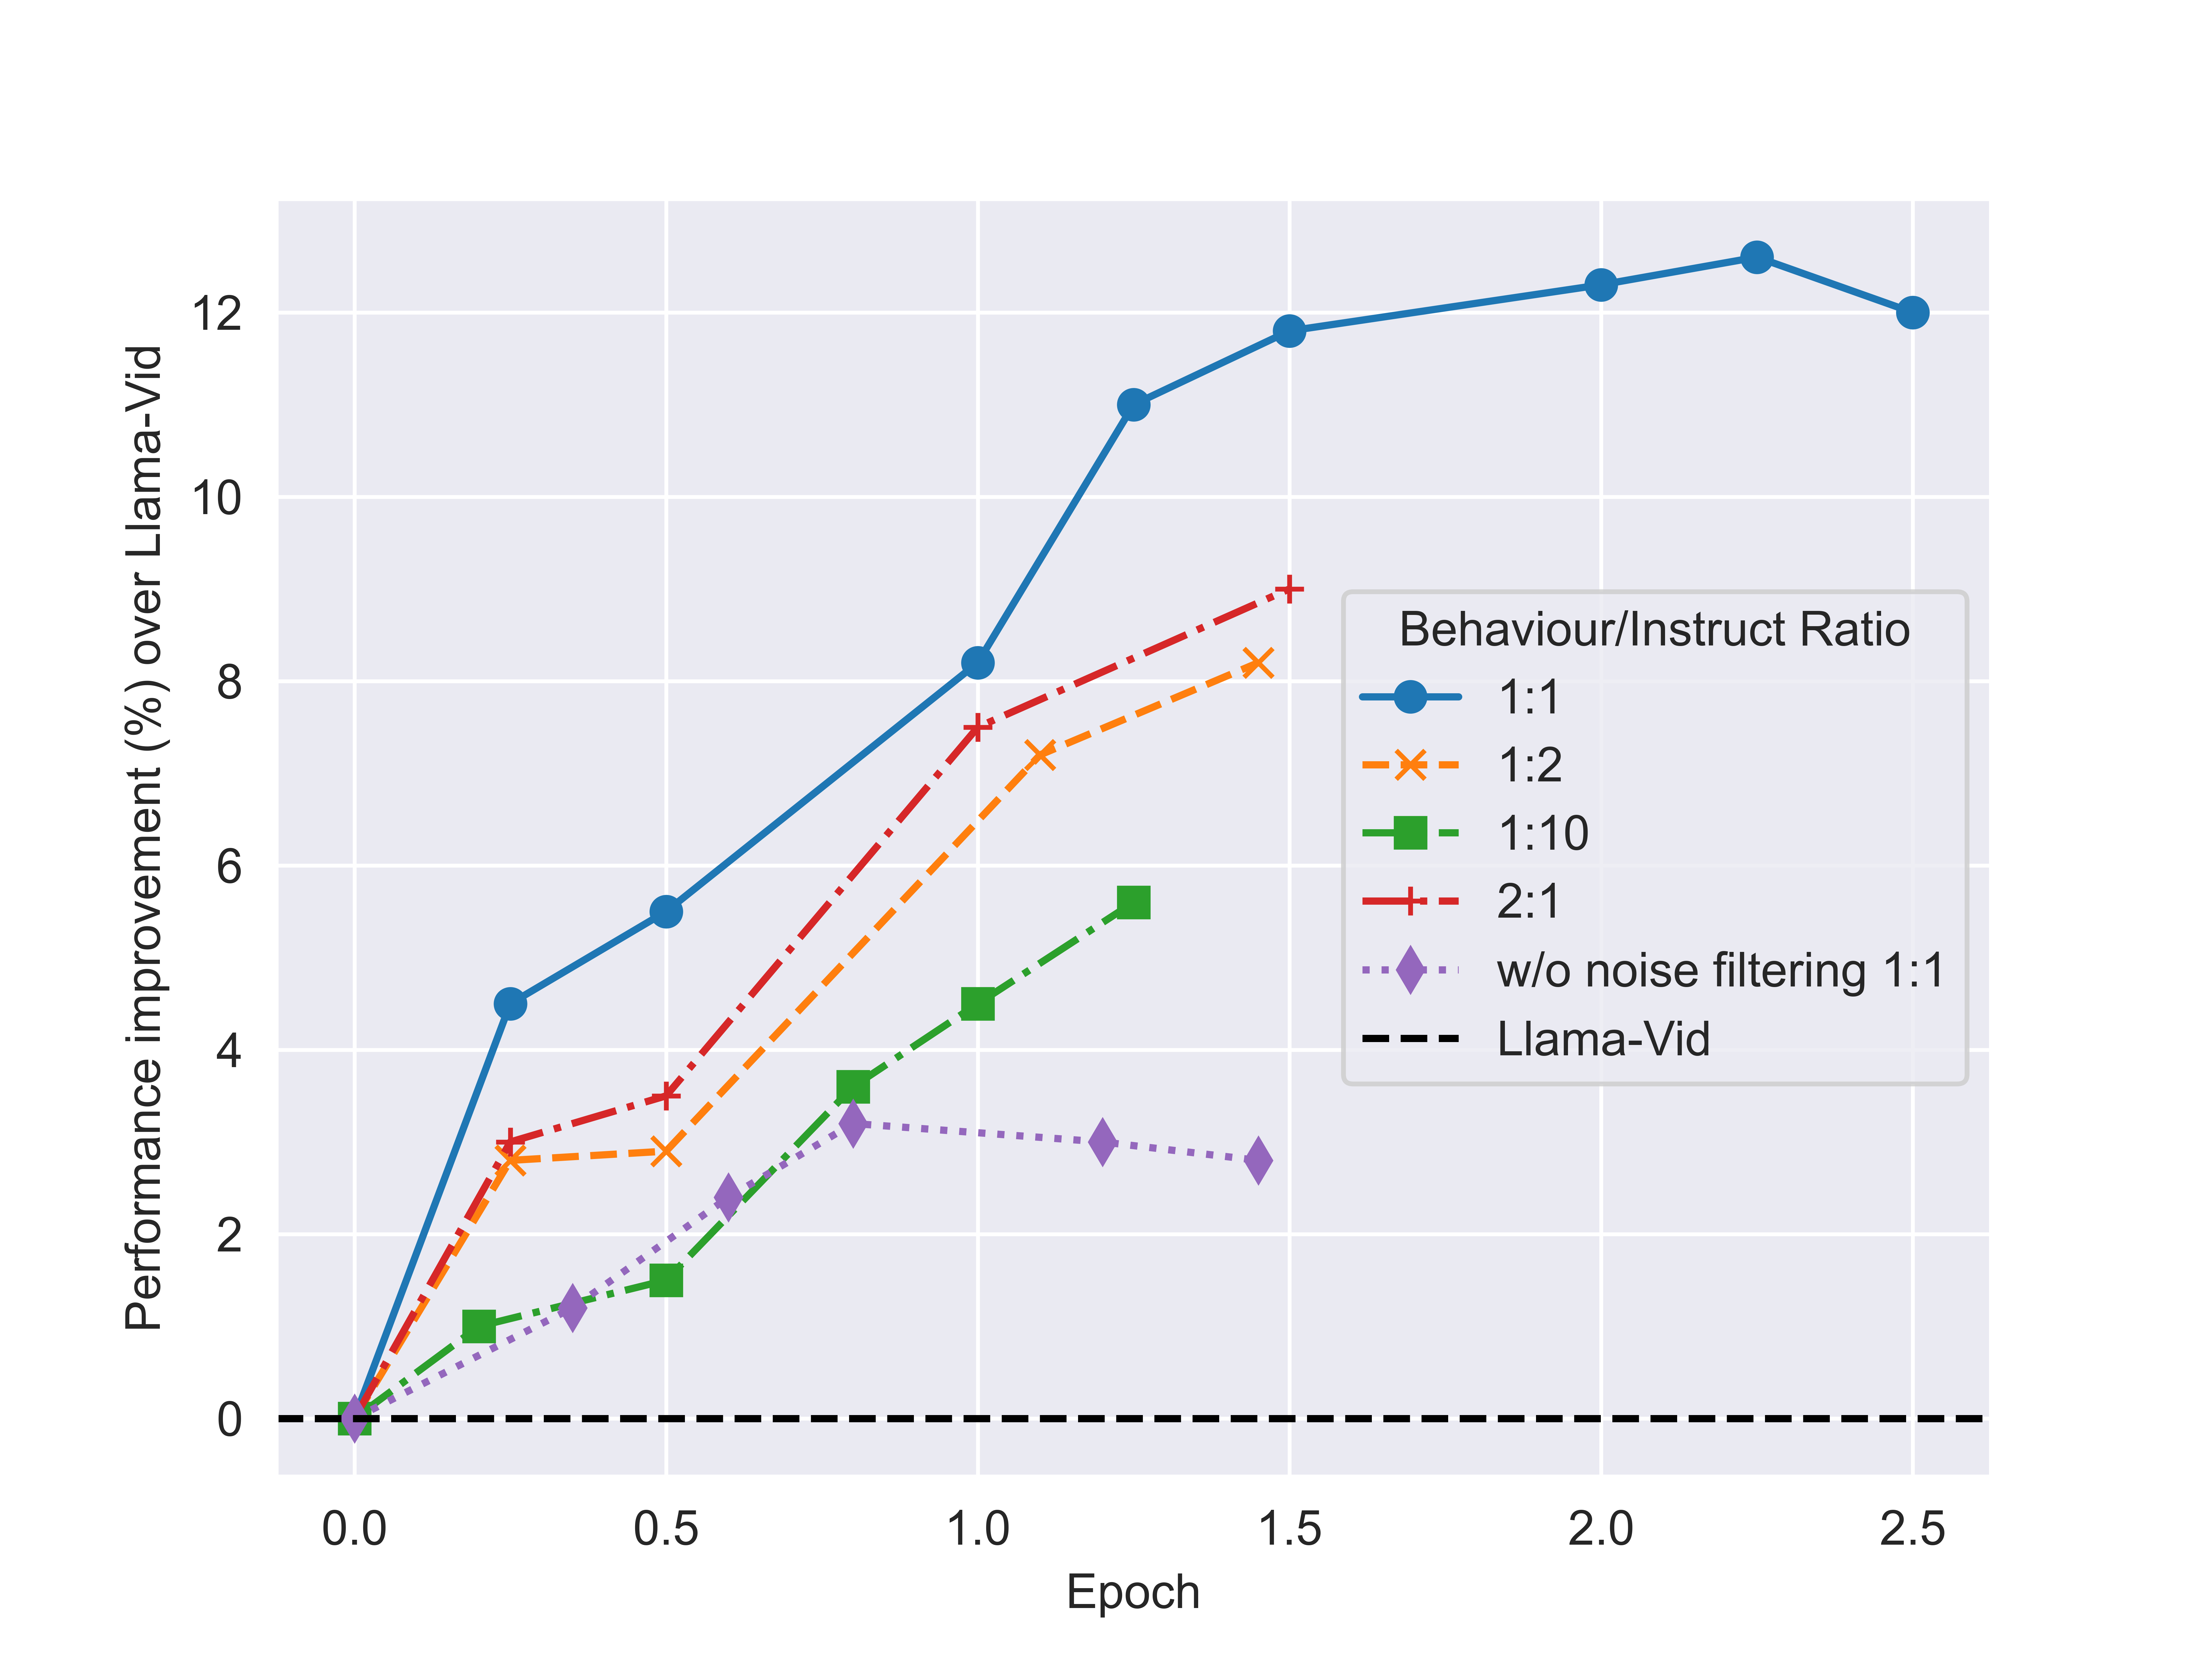
\includegraphics[width=0.9\linewidth]{images/performance_vs_epoch.png}
    \caption{Percentage performance improvement over an untrained LLaMA-Vid model, compared across various sampling ratios at different checkpoints. The 1:1 sampling ratio shows the best empirical performance. Performance is averaged over 0-shot accuracy improvements on six tasks with 250 samples each from the evaluation set. These tasks include image emotion recognition, video emotion recognition, and persuasion strategy classification, MSRVTT, HVU and MSVD-QA. The figure also shows the benefit of our data filtering process. While training on unfiltered BLIFT also improves the result over baseline performance of Llama-Vid but data filtering adds more improvement on top of it.}
    \label{fig:eval-ablation}
\end{figure}


\subsubsection{Instruction Fine-Tuning LLaMA-Vid}
After collecting Reddit and YouTube media and user behavior, we formulate instruction fine-tuning tasks for training LLaMA-Vid. In the training instruction, given the media content and automatic speech recognition if available, we ask the model to simulate the scene-by-scene description and user likes/views and top-5 comments. This instruction training template is given in Listing~\ref{lst:blift-template}. 
To generate the instruction data, first, frames are sampled using the 30-degree rule \cite{si2023long,arev2014automatic,friedman2004knowledge}, then the scene-by-scene description are obtained by concatenating automatically generated captions and tags from LLaVA-13B \cite{liu2023visual}, colors and tone through \citet{qin2020u2}. This instruction format keeps the instructions similar to the instruction format for other VLMs like LLaVA \cite{liu2023visual}, MiniGPT-4 \cite{zhu2023minigpt}, BLIP \cite{li2022blip}, LLaMA-Vid \cite{li2023llamavid}, \textit{etc.}, while additionally teaching the model to learn behavior. We keep the instruction fine-tuning template similar for both YouTube and Reddit. The complete instruction is given in Listing~\ref{lst:blift-template}. 



We start with the trained LLaMA-Vid model. The LLaMA-Vid model uses two tokens to represent each frame in the video, which they call content and context tokens. While the context token encodes the overall image context based on user input, the content token encapsulates visual cues in each frame. For learning context tokens, the model uses attention queries that interact with previously generated image features in the designed attention module. To generate content tokens, the image features are average pooled.
This dual-token strategy significantly reduces the number of tokens needed to represent videos, thus enabling the model to scale to longer (hour-long) videos. To better support hour-long videos, LLaMA-Vid was trained on a 9k movie-level conversation instruction set containing plot reasoning and detail understanding questions. 


Taking the base LLaMA-Vid model, we finetune it further on behavioral data. % We teach the model that given a media file (image or a video), it has to simulate the likes and comments on the media (Listing~\ref{lst:blift-template}). We do this on a 730k instructions set created by us using Reddit and YouTube videos and images (\S\ref{sec:methodology}). 
In our experiments we observe that the sampling ratio of BLIFT and IFT datasets is an important hyperparameter. We track 4 zero-shot metrics, likes/views, comments perplexity, and empirically find the best results with 1:1 ratio for 2.2 epochs (see Fig~\ref{fig:eval-ablation} and Table~\ref{tab:eval-ablation}). For the best checkpoint, the perplexity on comments reduces from 6.22 to 3.05, and the R2
on likes/views goes from -5.1 to 0.45

 We combine 730k instruction pairs from BLIFT with the original instruction tuning dataset consisting of 40K text conversations from ShareGPT, 625K single or multi-turn visual QA pairs, and 98K video QA pairs; all the modules except the Visual Encoder are kept frozen. We ablate on multiple sampling ratios from BLIFT. We train the LLaMA-Vid checkpoints with their original SFT mix along with BLIFT. We ablate different sampling ratios and found 1:1 to be empirically performing the best. We train the model for 2.2 epochs, keeping track of the 0-shot evaluation metrics and perplexity on comments in the eval set %\cy{Did you do fully finetuning or adaptation such as LoRA? If former, did you try LoRA?}. 
 Fig~\ref{fig:eval-ablation} and Table~\ref{tab:eval-ablation} show the ablations on different sampling ratios and epochs of training. 
For the best checkpoint, the perplexity on comments reduces from 6.22 to 3.05, and the $R^2$ on likes/views goes from -5.1 to 0.45.




\begin{table}[]
\centering
\begin{adjustbox}{width=\textwidth}
\begin{tabular}{l|lllll}
\toprule[1.2pt]
\textbf{Task}  & \textbf{MSRVTT-QA} & \textbf{CAER} & \textbf{Emoset} & \textbf{Comments} & \textbf{likes/views}\\ \midrule[1.2pt]
Base & 58.9 & 75.6 & 45.23 & 6.22 & -0.1\\
Salicon [Region] & 55.6 & 75.8 & 47.25 & 6.25 & -0.07\\
Salicon [Object] & 57.9 & 76.4 & 48.0 & 6.12 & 0.05\\
BLIFT[Likes/Views] & 58.2 & 76.2 & 47.12 & 6.15 & 0.38\\
BLIFT[Titles] & 58.4 & 78.1 & 48.12 & 5.09 & 0.13\\
BLIFT[Comments] & 59.0 & 79.1 & 49.58 & 3.02 & 0.19\\
BLIFT & 59.2 & 79.3 &50.38 & 3.05 & 0.40\\
%Salicon [Region] + BLIFT & 59.1 & 50.05 & 4.75 & 0.31\\
%Salicon [Object] + BLIFT & 59.1 & 50.31 & 4.02 & 0.35\\

%\hline
%Social-Captioning & GPT4-V &  &  &  \\
%& LLaVA-1.6 (34B) &  &  &  \\
%& LLaMA-Vid (13B) &  &  & \\
%& Behavior-LLaVA (13B & &  &  \\
\bottomrule[1.2pt]
\end{tabular}
\end{adjustbox}
\caption{Ablation on using comments and/or perception signals from Salicon \label{tab:salicon-ablation}}
\end{table}

\begin{table}[]
\centering
\begin{adjustbox}{width=\textwidth}
\begin{tabular}{ll|cccc}
\toprule[1.2pt]
\textbf{Sampling Ratio}  & \textbf{Epoch} & \textbf{Likes/Views $R^2$} & \textbf{Comments Perplexity} & \textbf{Performance}\\ \midrule[1.2pt]
Base-Model & 0 & -0.1 & 6.22 & 0\\
\midrule
\multirow{6}{*}{1:1} & 0.5 & 0.11 & 4.71 & 5.49\\
& 1 & 0.22 & 3.95 & 8.23\\
& 1.25 & 0.33 & 3.19 & 10.97\\
& 1.5 & 0.35 & 3.13 & 11.79\\
& 2 & 0.38 & 3.08 & 12.31\\
& 2.2 & 0.4 & 3.05 & 12.57\\
\midrule
\multirow{3}{*}{1:2} & 0.5 & 0.14 & 4.33 & 3.04\\
& 1.05 & 0.28 & 3.66 & 7.08\\
& 1.45 & 0.42 & 2.99 & 8.12\\
\midrule
\multirow{4}{*}{1:10} & 0.5 & 0.15 & 3.43 & 1.38\\
& 0.8 & 0.31 & 2.78 & 3.44\\
& 1 & 0.38 & 2.46 & 4.48\\
& 1.2 & 0.46 & 2.13 & 5.51\\
\midrule
\multirow{3}{*}{2:1} & 0.5 & 0.1 & 5.3 & 3.52\\
& 1 & 0.21 & 4.6 & 7.45\\
& 1.5 & 0.31 & 3.9 & 9.13\\
\bottomrule[1.2pt]
\end{tabular}
\end{adjustbox}
\caption{Ablation on different sampling ratios and epochs of training. Sampling ratio is the ratio of behaviour data to multimodal instruct data. Performance is the average increase in 0-shot accuracy on 6 tasks with 250 samples each from the eval set. These tasks include image emotion recognition, video emotion recognition, persuasion strategy classification, MSRVTT, HVU and MSVD-QA \label{tab:eval-ablation}}
\end{table}




%Next, we test the resultant model which we call Behavior-LLaVA, on a hierarchy of tasks in both zero-shot and finetuned settings. We include tasks based on low-level content understanding, like object and activity detection, and also on high-level understanding, like topic, sentiment, emotion, and persuasion classification. We also test the model on even higher-level tasks like memorability simulation and YouTube dislike/like simulation. We compare Behavior-LLaVA against the base model LLaMA-Vid and other state-of-the-art approaches reported on each test task (Tables \ref{table:lvu-benchmark}-\ref{tab:memorability}). 





\textbf{AdLLaVA to show the impact of behavior data:} To disentangle the effect of training on additional data samples from the effect of training on behavioral data, we train LLaMA-Vid on BLIFT with the video and image verbalization and do not include receiver behavior. Then, the overall instruction template consists of scene-by-scene automatically generated verbalization similar to Listing~\ref{lst:blift-template} without the likes and comment simulation. We call the LLaMA-Vid fine-tuned on this data, Ad-LLaVA. We compare Behavior-LLaVA with Ad-LLaVA and LLaMA-Vid along with other state-of-the-art literature benchmarks on various tasks (Tables \ref{table:lvu-benchmark}-\ref{tab:memorability}).





% \begin{lstlisting}[caption={Behavior Instruction fine-tuning template for the video: \url{https://www.youtube.com/watch?v=BKPQkjRF4yY}},frame=single,breaklines=true,basicstyle=\scriptsize, label={lst:blift-template}]
% <SYSTEM>You are an AI visual assistant, you are given a detailed description of a media, followed by the actual media. Answer all questions as you are seeing the media<SYSTEM><USER>The video advertisement is titled "Gatorade | Make Your Own Footsteps with Suni Lee " for the brand Gatorade. The audio in the ad says "A role model isn't just someone who looks like you, or comes from your place. There's someone who feels what you do. Someone who shows what's possible when you believe within. Not because you need to follow someone else's footsteps. But as a reminder to make your own. www.circlelineartschool.com" The scene by scene descriptions are Scene 1: The scene shows a woman looking off into the distance with an orange line going around the outside of the screen. The foreground colors of the scene are Black,Mud_Green,Gray,Dark_Gray, and the background colors are Dark_Brown,Black,Dark_Gray. The dominant tone of the scene is neutral. This scene is categorized by the tags cosmetic, eyebrow, face, girl, ponytail, stand, string, woman.
% Scene 2: The scene shows a woman balancing on a skate board in a yard. The foreground colors of the scene are Black,Mud_Green,Dark_Gray,Olive, and the background colors are Black,Dark_Gray,Gray,Dark_Brown. The dominant tone of the scene is neutral. This scene is categorized by the tags athletic, balance, beam, car, girl, house exterior, hurdle, jog, legging, plank, rail, seesaw, woman, yard.
% Scene 3: The scene shows a girl jumping over a wooden ramp in the backyard. The foreground colors of the scene are Black,Dark_Gray,Gray,Dark_Blue, and the background colors are Dark_Brown,Dark_Blue,Purple,Dark_Pink,Brown. The dominant tone of the scene is neutral. This scene is categorized by the tags arm, backyard, balance, diving board, girl, house exterior, ledge, plank, purple, rail, shirt, short, stand, stretch, woman, yard.
% Scene 4: The scene shows the woman poses with her arms extended in front of her. The foreground colors of the scene are Gray, and the background colors are Black,Dark_Blue,Dark_Brown,White,Gray. The dominant tone of the scene is neutral. This scene is categorized by the tags athletic, crop top, hand, girl, gym, gymnast, legging, leotard, muscle, ponytail, stand, stretch, text, tight, woman. The text shown in the scene is '"WHAT'SINSIDE SUNIIS INSIDE YOU"'
% Scene 5: The scene shows a couple of people jumping in a swimming pool. The foreground colors of the scene are Black, and the background colors are Brown,Orange,Khaki,Dark_Brown,Dark_Green. The dominant tone of the scene is neutral. This scene is categorized by the tags athletic, swimwear, bikini, dive, diving board, flip, girl, jump, person, pool, swimmer, swimming pool, woman.
% Scene 6: The scene shows a man is hanging from a skateboard on top of a field. The foreground colors of the scene are Mud_Green,Olive, and the background colors are Black,Gray,Khaki. The dominant tone of the scene is neutral. This scene is categorized by the tags belly, athletic, floor, girl, grass, person, lay, pole, rail, stand, stomach, stretch, tree, woman.
% Scene 7: The scene shows a woman in black clothes doing a hand stand on top of a yellow skateboard. The foreground colors of the scene are Black,Dark_Gray,Gray,Cyan, and the background colors are Black,Dark_Brown. The dominant tone of the scene is neutral. This scene is categorized by the tags athletic, balance, bend, flip, floor, gymnast, handstand, jump, leotard, man, mat, ramp, skateboarder, stretch, trick, woman.
% Scene 8: The scene shows a woman wearing a black top stands in front of a building. The foreground colors of the scene are Black,Dark_Gray,Gray,Mud_Green, and the background colors are Black,Dark_Blue,Brown,White,Khaki. The dominant tone of the scene is neutral. This scene is categorized by the tags athletic, crop top, girl, hip, jog, muscle, ponytail, shirt, stand, tight, waist, woman. The text shown in the scene is 'MORE ROLEMODEL STORIES', 'FUEL', 'TOMORROW' 
% Scene 9: The scene shows a man with a bike and house with the words fuel tomorrow on it. The foreground colors of the scene are Black,Dark_Gray,Gray, and the background colors are Black,Gray,White,Dark_Gray,Dark_Brown. The dominant tone of the scene is neutral. This scene is categorized by the tags green, man, shirt, stand. The text shown in the scene is 'FUEL', 'TOMORROW', 'BOLTDes' 
% Scene 10: The scene shows a woman is posing with the text fuel tomorrow. The foreground colors of the scene are Gray,Dark_Gray,Dark_Brown, and the background colors are Dark_Green,Dark_Brown,White,Dark_Blue,Black. The dominant tone of the scene is neutral. This scene is categorized by the tags belly, athletic, girl, hip, muscle, pose, room, shirt, stand, vest, woman. The text shown in the scene is 'FUEL', 'TOMORROW'
% Analyze this video deeply and answer the following questions. What percentage of viewers would like this video, and what would be the top-5 popular comments on this video?.<USER><ASSISTANT>The video will be liked by 2.0% viewers and the popular comments could be:
% 1. "Wow. Love it. She's such an inspiration to the the next generation as well as everyone.:purple-heart:confetti"
% 2. "Inspiring and great story behind this commercial. Builds meaning and purpose in the hearts and mind of youth. It's been awhile since good meaningful ads have been made."
% 3. "She's an inspiration ️ to the world  ️ thanks to her my niece learning Gymnastics hopefully someday, she is an inspiration to other youngers as how suni is an inspiration to everyone "
% 4. "Chills watching this. Such an inspiration:heart"
% 5. "Yooooo, this is straight up :fire:fire:fire:fire!"
% \end{lstlisting}



\textbf{Impact of filtering steps on performance:} We use various filtering steps in our data pipeline, including NSFW filters, time filters, bot filters, and gaming and news video filters. To quantify the impact of our filtering steps on the final performance, we compare the performance from training on unfiltered data with filtered data (Figure \ref{fig:eval-ablation}).
The figure shows the benefit of our data filtering
process. While training on unfiltered BLIFT also improves the result over baseline performance of Llama-Vid
but data filtering adds more improvement on top of it

\textbf{Ablation with perceptual behavior:} As an ablation experiment, we also try teaching the Behavior-LLaVA perceptual signals. For this, we take the largest perception signal dataset in the literature - Salicon10k \cite{jiang2015salicon}. It consists of 10,000 MS COCO images \cite{chen2015microsoft} with free-viewing eye gaze data collected through a novel mouse-based interface. The dataset has been widely used in many studies. We formulate two tasks using this data, (1)~\textbf{Salicon [Object]}: estimating the saliency over the objects in the image and (2)~\textbf{Salicon [Region]}: estimating the saliency over a region, where the regions tiles formed by breaking the image into a 3x3 grid. For both tasks we try to model two objectives, ranking and predicting, we found ranking to be much more effective. The instruction are given in Listings~\ref{lst:blift-template-perceptual} and \ref{lst:blift-template-perceptual-region}.




\begin{figure}[!h]
\begin{minipage}[c]{0.3\textwidth}
        \centering
        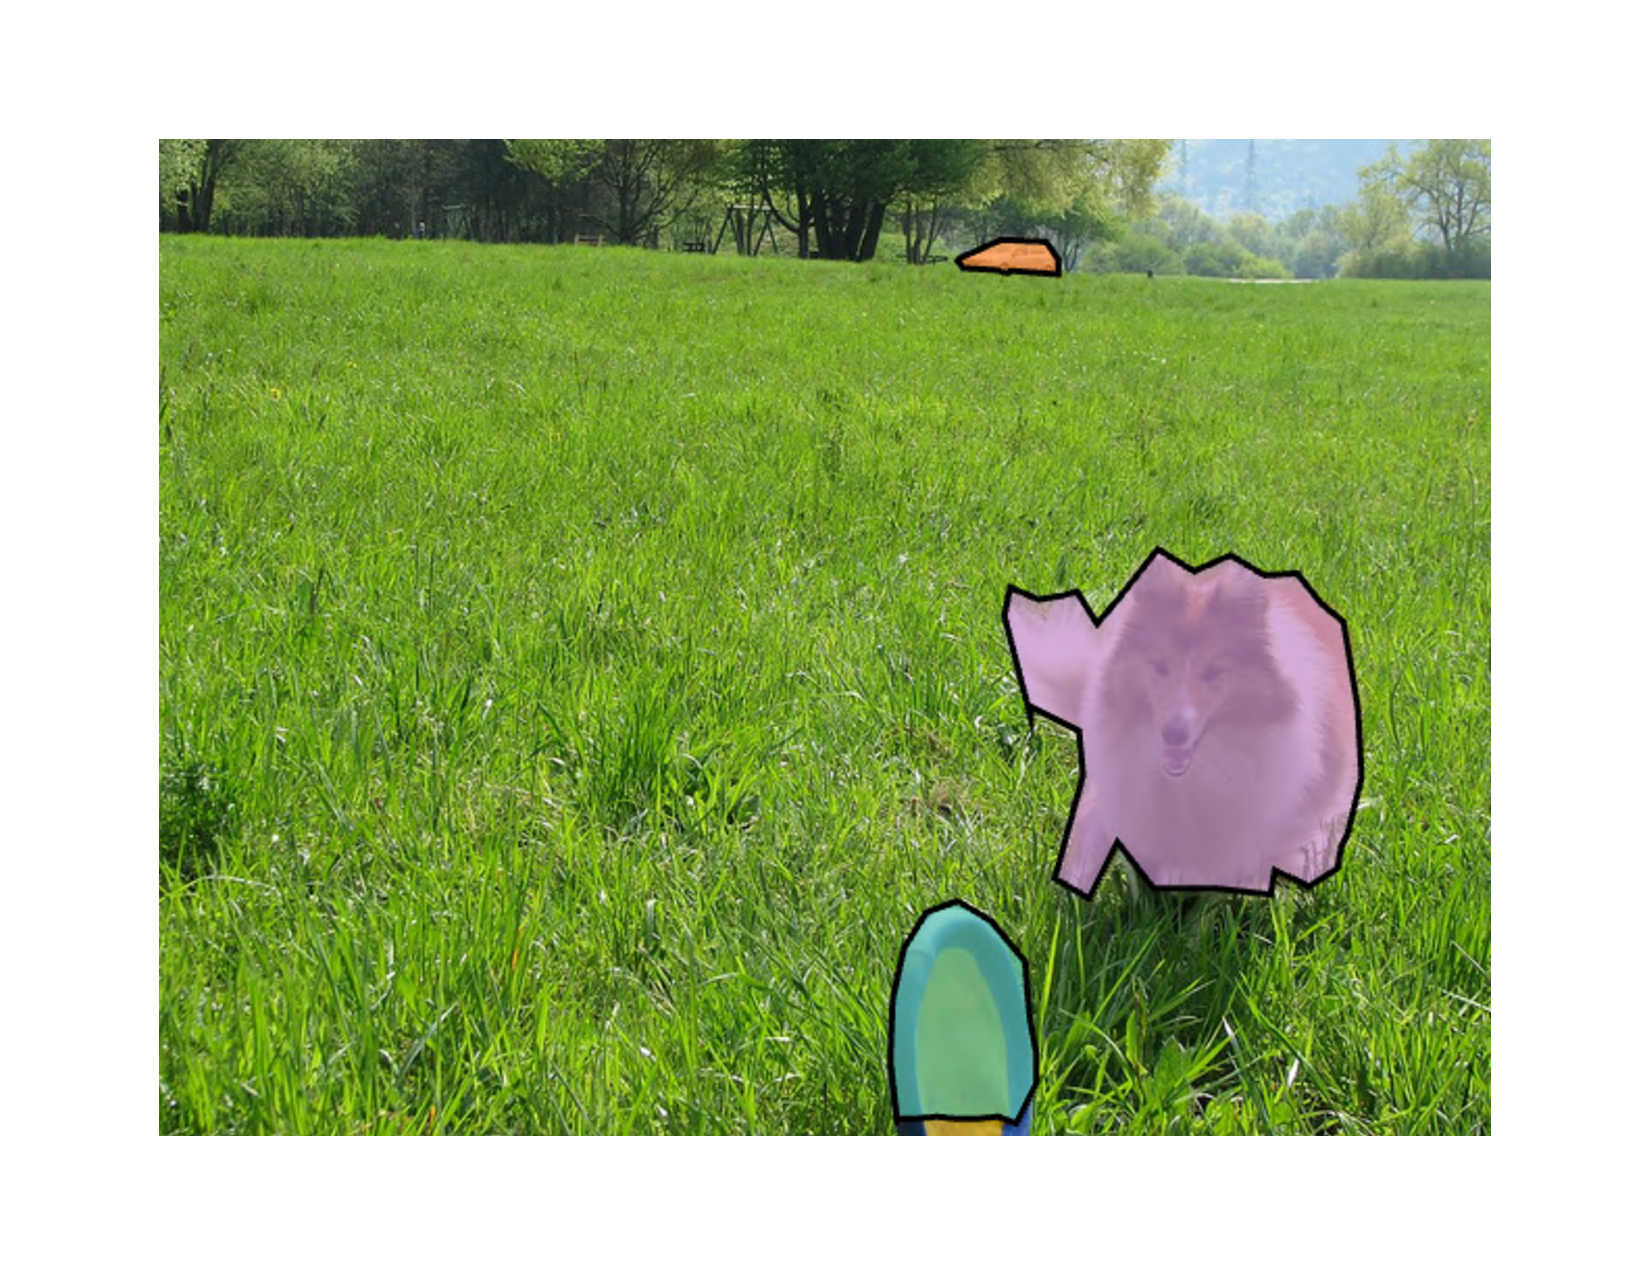
\includegraphics[width=\textwidth]{images/listing-image_compressed.pdf}
    \end{minipage}
    \hfill
    \begin{minipage}[c]{0.67\textwidth}
\small
\centering
\scriptsize
\begin{lstlisting}[caption={Perceptual Signal Instruction fine-tuning template for the image: \url{http://farm6.staticflickr.com/5106/5670500150_e035dd2d30_z.jpg}},frame=single,breaklines=true,basicstyle=\scriptsize, label={lst:blift-template-perceptual}]
<SYSTEM>You are an AI visual assistant. Answer all questions as you are seeing the media<SYSTEM><USER>The objects in this image in no particular order are car, dog, frisbee. Give me the order of saliency of these objects, start with the most salient object and end with the least salient object, each in a separate line. Give me the objects only and nothing else.
<image>
<ASSISTANT>
dog
frisbee
car
<ASSISTANT>
\end{lstlisting}
\end{minipage}
\label{fig:listing-perception-image}
\end{figure}


\begin{figure}[!h]
\begin{minipage}[c]{0.3\textwidth}
        \centering
        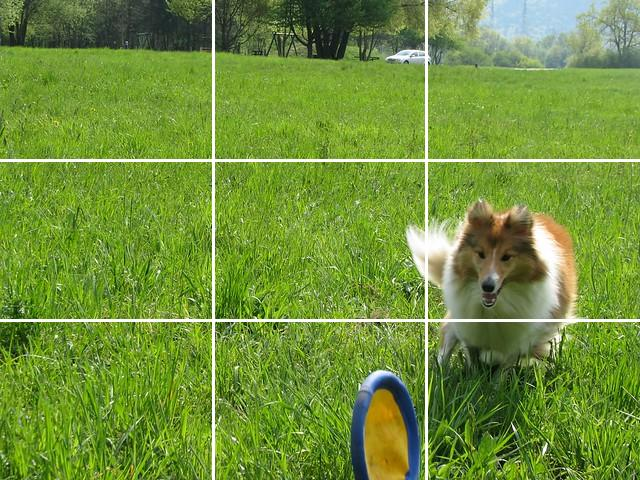
\includegraphics[width=\textwidth]{images/listing-image-grid.jpg}
    \end{minipage}
    \hfill
    \begin{minipage}[c]{0.67\textwidth}
\small
\centering
\scriptsize
\begin{lstlisting}[caption={Perceptual Signal Instruction fine-tuning template for the image: \url{http://farm6.staticflickr.com/5106/5670500150_e035dd2d30_z.jpg}},frame=single,breaklines=true,basicstyle=\scriptsize, label={lst:blift-template-perceptual-region}]
<SYSTEM>You are an AI visual assistant. Answer all questions as you are seeing the media<SYSTEM><USER>Assume the given image is broken into a 3X3 grid the regions or tiles being named "upper-left" "upper-center", "upper-right", "middle-left", "middle-center", "middle-right", "bottom-left", "bottom-center", "bottom-right". Rank these regions or tiles based on their saliency, give me the line separated ranking of all regions in decreasing order.
<ASSISTANT>
middle-right
bottom-center
bottom-right
upper-center
upper-right
middle-center
upper-left
middle-left
bottom-left
\end{lstlisting}
\end{minipage}
\label{fig:listing-perception-image-region}
\end{figure}





% Apart from salient object we also tried salient region (by dividing the image into 3X3 grid namely top left, top middle, top right, .., and bottom right. From \ref{tab:salicon-ablation} we do not find conclusive evidence of performance improvements in the training / downstream tasks in 0-shot, the salient object detection tasks proves to be significantly better, improving the performance in image emotion recognition over the base model as well.

 

%ShareGPT original: 70k conversations from sharegpt

% ShareGPT multimodal: LLaVA instruction set (not including pretraining) : 556k multimodal conversations using GPT4

% VideoChatGPT: 130k Video Conversations uses GPT4




%We take the pretrained checkpoints of the LLaMA-VID 13B \cite{li2023llama} model after the modality-alignment stage.




\begin{landscape}
    
\begin{table*}[]
\centering
\begin{adjustbox}{max width=1.5\textwidth}
\begin{tabular}{llccccccccc}
\toprule[1.2pt]
\textbf{Model} & \textbf{scene} & \textbf{way\_speaking} & \textbf{relationship}   & \textbf{like\_ratio} & \textbf{view\_count} & \textbf{director} & \textbf{genre} & \textbf{writer} & \textbf{year} \\
\midrule[1.2pt]
%Trained & R101-slowfast+NL  & 52.4 & 35.8 & 54.7 & 0.386 & \valgood{3.77} & 44.9 & 53.0 & 36.3 & 52.5 \\
% Trained & VideoBert  & 52.8 & 37.9 & 54.9 & 0.320 & 4.46 & 47.3 & 51.9 & 38.5 & 36.1 \\
%Trained  & Xiao et. al (2022) & 50.95 & 34.07 & 44.19 & 0.353 & 4.886 & 40.19 & 48.11 & 31.43 & 29.65 \\
% Trained & Qian et. al (2021) & 50.95 & 32.86 & 32.56 & 0.444 & 4.600 & 37.76 & 48.17 & 27.26 & 25.31 \\
%Trained & Object Transformers & 53.1 & \valbest{39.4} & 56.9 & 0.230 & \valbest{3.55} & 51.2 & \valgood{54.6} & 34.5 & 39.1 \\ 
%Trained & Video4096- GPT-3.5 generated story + Roberta & 62.16 &  38.41 &  \valbest{68.65} &\valgood{0.054} & 11.84 & 45.34 & 39.27 & \valgood{35.93} & 7.826 \\
\makecell[l]{Video4096-GPT-3.5 generated story \\+ Flan-t5-xxl } & \valgood{60.2} & \valgood{39.07} & 64.1 &\valgood{0.061} & 12.84 & 69.9 & \valbest{58.1} & \valbest{52.4} & 75.6 \\
\makecell[l]{Video4096-GPT-3.5 generated story \\+ GPT-3.5 classifier } & 54.54 & 32.95 & \valbest{68.42} & \valbest{0.031} & 12.69 & \valbest{75.26} & 50.84 & 32.16 & \valgood{75.96} \\
LLaMA-Vid + GPT-3.5 Generated Story & 58.12 & 35.5  & 60.6 & 0.314 & \valgood{10.34} & 65.34 & 49.77 & 34.23 & 72.12\\
Ad-LLaVA & 59.05 & 37.07 & 61.2 & 0.319 & 10.37 & 66.84 & 55.13 & 35.33 & 77.34 \\
Behavior LLaVA + GPT-3.5 Generated Story & \valgood{66.43} & \valbest{41.03} & \valbest{64.21} & 0.17 & \valbest{5.12} & \valgood{71.12} & \valbest{63.45} & \valgood{39.4} & \valbest{79.3}\\\hline
\textbf{\makecell[l]{Improvement of Behavior LLaVA \\ over LLaMA-Vid}} & \textcolor{ForestGreen}{10.48\%} &  \textcolor{ForestGreen}{15.58\%}& \textcolor{ForestGreen}{9.62\%}&  \textcolor{ForestGreen}{45.86\%}&  \textcolor{ForestGreen}{50.48\%}&  \textcolor{ForestGreen}{8.85\%}&  \textcolor{ForestGreen}{27.49\%}& \textcolor{ForestGreen}{15.1\%}& \textcolor{ForestGreen}{9.96\%}\\
\bottomrule[1.2pt]
\end{tabular}
\end{adjustbox}
\caption{Comparison of various models on the Long Video Understanding benchmark \cite{wu2021towards} consisting of 9 VQA tasks. We see that Behavior-LLaVA improves on LLaMA-Vid on 9/9 tasks with an average improvement of 21.49\%. Further, it outperforms the state-of-the-art in 5/9 tasks.\label{table:lvu-benchmark} %\cy{The font is too small. The ``Model'' column takes up too much space, maybe each model description can use two rows. Same applies to other tables.}
}
\end{table*}

\end{landscape}







%%%%%%%%%%%%%%%%%%%%%%%%%%%%%%%%%%
%%%%%%%%%%%%%%%%%%%%%%%%%%%%%%%
%%%%%%%%%%%%%%%%%%%%%%%%%%%%%%%%%%%%%
%%%%%%%%%%%%%%%%%%%%%%%%%%%%%%%%%%
%%%%%%%%%%%%%%%%%%%%%%%%%%%%%%%%%%
%%%%%%%%%%%%%%%%%%%%%%%%%%%%%%%%%%
\subsection{Results and Discussion}
In the experimental results, we aim to showcase the diverse and emergent capabilities of our Behavior-LLaVA model through quantitative numbers on various tasks and qualitative examples. These abilities include generating detailed image and video descriptions, emotion and sentiment analysis, question answering, video understanding tasks like scene and action detection. Additionally, we present the ability of Behavior-LLaVA to transfer learn on other behaviors like memorability of a video - both short-term and long-term. 

\begin{comment}
    
With Behaviour Understanding (comments generation): Content Understanding (0-shot content tasks) :: 10:1

At 1 epoch: BU is bad (incoherent comments), but CU is good
At 1.5 epochs BU is good (coherent comments), but CU drops significantly (~5\% for memorability and emotions)

\begin{enumerate}
    \item 400k rpics verbalized + title comments + emotions
    \item 100k Emotion net verbalization + emotions
    \item setting up BLEU for evaluation
    \item LLM Training
    \item LLaVA Training
    \item Video-Emotion Tags (youtube80k, adsotw, rvideos) \~200k
    
    \item downstream benchmarks

    \item 
\end{enumerate}

\end{comment}





\subsubsection{Evaluation}

To test the effectiveness of Behavior-LLaVA, we conduct experiments involving 46 distinct tasks across 26 benchmark datasets. The diversity of tasks and datasets allows us to evaluate the performance and capabilities of Behavior-LLaVA thoroughly. Each of them is covered briefly next:










\begin{enumerate}[wide]
    \item \textbf{Visual Question Answering (VQA)}: We evaluate the performance of visual question answering on the following benchmark datasets:

    \begin{itemize}
         
        \item The Long-Video Understanding (LVU) benchmark by \citet{wu2021towards} comprises nine distinct tasks aimed at assessing long video comprehension, incorporating over 1000 hours of video content. These tasks encompass diverse aspects such as content understanding (including relationship, speaking style, scene/place), prediction of user engagement (YouTube like ratio, YouTube popularity), and movie metadata (director, genre, writer, movie release year). %Evaluation of LVU tasks by \citet{wu2021towards} utilizes top-1 classification accuracy for content understanding and metadata prediction tasks, while Mean Squared Error (MSE) is employed for user engagement prediction tasks.
    
        \item The Holistic Video Understanding (HVU) dataset by \citet{diba2020large} stands as the largest dataset for long video comprehension, comprising 572,000 samples. Encompassing a broad spectrum of semantic elements within videos, HVU tasks involve the classification of scenes, objects, actions, events, attributes, and concepts. Performance evaluation on HVU tasks is conducted using the mean average precision (mAP) metric on the validation set.

        \item We also use MSVD-QA, MSRVTT-QA \cite{chen2011collecting,xu2016msr}, and ActivityNet-QA \cite{caba2015activitynet} datasets. Their description is given in Appendix~\ref{sec:Dataset Descriptions}. 
        
    \end{itemize}
   

    \item \textbf{Video and Image Understanding Benchmarks}: We use a wide variety of tasks to evaluate video and image understanding: topic, emotion, and persuasion strategy classification, action and reason retrieval and generation, and emotions. We briefly introduce the benchmarks:
    
        \begin{itemize}
            \item The advertisements dataset by \citet{hussain2017automatic} contains 3,477 video advertisements and the corresponding annotations for emotion and topic tags and action-reason statements for each video. There are a total of 38 topics and 30 unique emotion tags per video. Further, we have 5 action-reason statements for each video for the action-reason generation task. %For our experiment, we use 1785 videos, due to other videos being unavailable/privated from Youtube.

            \item Persuasion strategy dataset \cite{bhattacharya2023video} is a dataset consisting of 1002 video advertisements from popular brands and their persuasion strategy labels like social identity, anchoring and comparison, reciprocity, foot-in-the-door, \textit{etc}.



        \item For emotion analysis, we use VideoEmotion-8 \cite{asur2010predicting}, Ekman-6 \cite{xu2016heterogeneous}, CAER \cite{lee2019context}, IAPSa \cite{mikels2005emotional}, Emotion6 \cite{peng2015mixed}, EmoSet \cite{yang2023emoset}, and Abstract \cite{machajdik2010affective} datasets. A brief description for each of them is given in Appendix~\ref{sec:Dataset Descriptions}.

    
        \end{itemize}

    \item \textbf{Image Dense Captioning}: Literature image captioning datasets such as MS-COCO \cite{chen2015microsoft} reduce the inherently rich information and fine-grained semantics to simplistic captions, with very brief statements focussing only on salient objects. Behavior data such as user comments help a model learn much more information such as object and material properties, world knowledge, emotion, character understanding, spatial relationships, aesthetics, \textit{etc.} (see Fig.~\ref{fig:synthetic-data-vs-generation-performance}), enhancing the model's captioning capability. Therefore, we design a captioning task to test this capability and compare it with respect to LLaMA-Vid and LLaVA-34B (a 2.5x larger model). Since we do not have ground truth for this task, following the LLM-as-a-judge paradigm, we use GPT-4V as the judge for all the models. GPT-4V is asked to evaluate the dense captions on three metrics: \textit{Correctness} (Listing~\ref{lst:dense-caption-correctness}) evaluating the factuality and model hallucinations, \textit{Detail} (Listing~\ref{lst:dense-caption-detail}) evaluating the number and depth of details captured by the generated captions, and \textit{Quality} (Listing~\ref{lst:dense-caption-quality}) measuring the subjective quality of the concepts chosen to be highlighted by the captioning model and the arrangement, coherence, and the linking of various concepts.



    \item \textbf{Image and Video Memorability Simulation}: Behavior-LLaVA is trained on behavior along with the media. To check if training on behavior helps in solving other behavior tasks \cite{khandelwal2023large}, we test it over image and video memorability simulation. For this, we select seven benchmark datasets covering long-term and short-term memorability over images and videos: LaMem \cite{khosla2015understanding},  SUN \cite{isola2011makes}, and MemCat \cite{goetschalckx2019memcat} for images and 
    Memento10k\cite{newman2020multimodal}, VideoMem \cite{cohendet2019videomem},  MediaEval \cite{Kiziltepe2021}, and LAMBDA \cite{si2023long} for videos. We briefly cover each of them in Appendix~\ref{sec:Dataset Descriptions}.




    \item \textbf{Modalities other than videos and images:} Behavior-LLaVA, built on top of LLaMA-Vid and fine-tuned using BLIFT, is pretrained and fine-tuned on image and video datasets. To test if behavior data can improve the results on other modalities as well, we test Behavior-LLaVA's performance on two tasks across audio and text modalities (Table \ref{tab:modality-ablation}). For audio, we evaluate on the audio summarization task \cite{han2023shot2story20k} and for text, we evaluate on the IMDB sentiment benchmark \cite{maas-EtAl:2011:ACL-HLT2011}.

\end{enumerate}

For Tables~\ref{table:lvu-benchmark}, \ref{table:hvu-benchmark}, and \ref{tab:ad-understanding-kovashka}, we follow the evaluation protocol of Video-4096 \cite{bhattacharya2023video}, for Table~\ref{tab:video-qa} we follow the evaluation protocol of LLaVA and LLaMA-VID. For Tables~\ref{tab:video-emotion}, \ref{tab:image-emotion}, and \ref{tab:memorability}, for 0-shot evaluation results, we use the logits of the next token from the given task vocabulary. For Table~\ref{tab:memorability}, we use the evaluation protocol by \cite{si2023long}.




\begin{table}
\centering
\begin{adjustbox}{width=\textwidth}
\begin{tabular}{ll|lll}
\toprule[1.2pt]
\textbf{Training} & \textbf{Dataset} & \textbf{Video Emotion-8} & \textbf{CAER}  &\textbf{Ekman-6}\\ \midrule[1.2pt]
Random & Random & 12.5 & 14.28 & 16.67 \\\hline
0-Shot& LLaMA-Vid & 29.7 & 27.2  & 37.33 \\ 
%& w likes &   & 31.2    &\\ 
%& w comments &   & 54.9      &\\
& Behavior-LLaVA & 41.35  & 51.0   & 49.33 \\ 
& Ad-LLaVA & 29.8  & 27.3 & 37.66 \\ 
\cline{2-5}
\multicolumn{2}{r|}{\textbf{Improvement of Behavior-LLaVA over LLaMA-Vid}} & \textcolor{ForestGreen}{39.22\%}& \textcolor{ForestGreen}{84.19\%}& \textcolor{ForestGreen}{32.14\%}\\
\hline
Finetuned & \citet{zhao2020end} & 54.5 & 78.3 & 55.3 \\
& \citet{zhang2023weakly}  & 57.3  & 80.1 & 58.2\\ 
& eMOTIONS \cite{wu2023emotions} &- &- & 53.12\\
& \citet{arevalo2017gated} &53.7 & 77.3 & 54.2\\
& \citet{qiu2020dual} & 53.3 & - & 57.3\\
& \citet{xu2016heterogeneous} & 52.6 & 77.9 & 55.6 \\
& LLaMA-Vid & 53.8  & 75.6 & 57.9 \\
& Ad-LLaVA & 54.1  & 76.1 & 57.8 \\
& Behavior-LLaVA & 56.9  & 79.3 & 58.4 \\\cline{2-5}
\multicolumn{2}{r|}{\textbf{Improvement of Behavior-LLaVA over LLaMA-Vid}} & \textcolor{ForestGreen}{5.76\%}& \textcolor{ForestGreen}{3.57\%}& \textcolor{ForestGreen}{0.86\%}\\
% 0-Shot & GPT-4V & & & \\
\bottomrule[1.2pt]
\end{tabular}
\end{adjustbox}
\caption{Comparison of various models on three video emotion understanding benchmarks (Video Emotion8 \cite{jiang2014predicting}, CAER \cite{lee2019context}, Ekman-6 \cite{xu2016heterogeneous}). The main goal of comparing on these benchmarks is to demonstrate Behavior-LLaVA's understanding of complex tasks like video emotions of long-form videos. We see that Behavior-LLaVA improves on LLaMA-Vid on 3/3 benchmarks with an average improvement score of \textcolor{ForestGreen}{51.85\%} in zero-shot and \textcolor{ForestGreen}{3.39\%} in fine-tuned settings. Further, it outperforms the current state-of-the-art on 3/3 benchmarks in zero-shot and 1/3 in fine-tuned settings.}
\label{tab:video-emotion}
\end{table}




\begin{table}[]
\centering
\begin{adjustbox}{max width=1.0\textwidth}
\begin{tabular}{l|ccccc}
\toprule[1.2pt]
\textbf{Model} & \multicolumn{3}{c}{\textbf{Audio Summarization (3 Shot)}} & 
\multicolumn{2}{c}{\textbf{IMDb Sentiment}}\\ 
& BLEU & ROUGE & METEOR & 0-shot & 1-shot \\
\midrule[1.2pt]
Behaviour-LLaVA & 19.0 & 25.1 & 39.3 & 84.1 & 90.2 \\
LLaMA-VID & 15.1 & 18.3 & 30.7 & 80.3 & 87.9\\
VALOR \cite{chen2023valorvisionaudiolanguageomniperceptionpretraining} & 6.6 & 10.0 & 23.9 & - & - \\\hline
\textbf{\makecell[l]{Improvement of Behavior-LLaVA\\over LLaMA-Vid}} & \textcolor{ForestGreen}{25\%} & \textcolor{ForestGreen}{37\%} & \textcolor{ForestGreen}{28.01\%} & \textcolor{ForestGreen}{4.73\%}&
\textcolor{ForestGreen}{2.61\%}\\

\bottomrule[1.2pt]
\end{tabular}
\end{adjustbox}
\caption{Evaluation on audio and text modalities. We evaluate on the audio summarization benchmark \cite{han2023shot2story20k} for audio and IMDB sentiment benchmark for text \cite{maas-EtAl:2011:ACL-HLT2011}.\label{tab:modality-ablation}}
\end{table}




\begin{landscape}


\begin{table*}
\centering
\begin{adjustbox}{max width=1.5\textwidth}
\begin{tabular}{llllllll}
\toprule[1.2pt]
\multirow{2}{*}{\textbf{Training}} & \multirow{2}{*}{\textbf{Model}} & \multirow{2}{*}{\textbf{Topic}} & \multicolumn{2}{c}{\textbf{Sentiment}} & \multirow{2}{*}{\textbf{Persuasion}} & \multirow{2}{*}{\textbf{Action}} & \multirow{2}{*}{\textbf{Reason}} \\
& & & \textbf{Clubbed} & \textbf{All labels} & & & \\
\midrule[1.2pt]

Random & Random & 2.63 & 3.37 & 14.3 & 8.37 & 3.34 & 3.33 \\
\hline

Zero-shot & VideoChat \cite{li2023videochat}  & 9.07 & 3.09 & 5.1 & 10.28 & - & - \\
 & Video4096 - GPT-3.5 Generated Story + GPT-3.5 Classifier  & 51.6 & 11.68 & 79.69 &  \valgood{35.02} &  66.27 & 59.59 \\
 %& Video4096 - GPT-3.5 Generated Story + Flan-t5-xxl Classifier \cite{bhattacharya2023video} & \valgood{60.5} & 10.8 & 79.10 &  33.41 &  \valbest{79.22} & \valbest{81.72} \\
%& Video4096 - GPT-3.5 Generated Story + Vicuna Classifier \cite{bhattacharya2023video} & 22.92 & 10.8 & 67.35 & 29.6 & 21.39 & 20.89 \\
%& Video4096 - Vicuna Generated Story + GPT-3.5 Classifier \cite{bhattacharya2023video} & 46.7 & 5.9 & \valbest{80.33} & 27.54 & 61.88 & 55.44 \\
%& Video4096 - Vicuna Generated Story + Flan-t5-xxl Classifier \cite{bhattacharya2023video} & 57.38 & 9.8 & 76.60 & 30.11 & \valgood{77.38} & \valgood{80.66}  \\
%& Video4096 - Vicuna Generated Story + Vicuna Classifier \cite{bhattacharya2023video} & 11.75 & 10.5 & 68.13 & 26.59 & 20.72 & 21.00  \\
& LCBM \cite{khandelwal2023large} & 42.17 & 7.08 & 58.83 & 32.83 & 39.55 & 27.91 \\
& LLaMA-VID w/ only video & 10.11 & 3.42 & 5.75 & 12.32 & 29.61 & 24.11 \\
& LLaMA-VID w/ video + GPT-3.5 Story & 42.72 & 11.05 & 64.02 & 32.07 & 37.76 & 42.33 \\\cline{2-8}
& Behavior-LLaVA w/ only video & 22.65 & 11.13 & 60.04 & 13.39 & 42.66 & 33.33\\
& Behavior-LLaVA w/ video + verbalization &46.34 & \valgood{11.7} & 64.13& 33.33&  52.06 & 52.03 \\
& Ad-LLaVA w/ video + GPT-3.5 story& 51.16 & 11.33 & 68.03 & 33.11 & 43.26 & 51.45 \\
& Behavior-LLaVA w/ video + GPT-3.5 story & \valbest{60.09} & \valbest{12.84} & \valbest{79.94} & \valbest{36.12} & 67.10 & 79.18 \\
\cline{2-8}
\multicolumn{2}{c}{\textbf{Improvement of Behavior-LLaVA over LLaMA-Vid}} & \textcolor{ForestGreen}{40.66\%} & \textcolor{ForestGreen}{16.2\%} & \textcolor{ForestGreen}{24.86\%} &  \textcolor{ForestGreen}{12.62\%} & \textcolor{ForestGreen}{77.7\%}& \textcolor{ForestGreen}{87.05\%}\\\hline


\multirow{1}{*}{Finetuned} & %VideoMAE \cite{tong2022videomae} & 24.72 & 29.72 & 85.55 & 11.17 & - & - \\
%& \citet{hussain2017automatic}  & 35.1 & 32.8 & - & - & 48.45 & - \\
%& Intern-Video \cite{wang2022internvideo} & 57.47 & \valgood{36.08} & \valbest{86.59} & 5.47 & 6.8 & - \\
 Video4096- Generated Story + Roberta Classifier  & \valbest{71.3} & 33.02 & 84.20 & 64.67 & 42.96 & 39.09 \\
& LLaMA-VID w/ video + verbalization & 59.13 & 32.11 & 79.15 & 50.93 & 50.32 & 30.13 \\
& LLaMA-VID w/ video + GPT-3.5 Story & 63.11 & 35.01 & 84.15 & 55.01 & 57.11 & 45.73 \\\cline{2-8}
& Behavior-LLaVA w/ only video  & 58.03 & 22.72 & 84.41 & 26.23 & 59.33 &51.45\\
& Behavior-LLaVA w/ video + verbalization  & 68.32 & 33.92 & 85.93 & \valgood{64.72} & \valgood{70.89} & \valgood{75.34} \\
& Ad-LLaVA w/ video + GPT-3.5 story & 66.34 & 36.24 & 84.09 & 58.31 & 68.15 & 78.15 \\
& Behavior-LLaVA w/ video + GPT-3.5 story & \valbest{71.2} & \valbest{39.55} & \valgood{86.17} & \valbest{65.03} & \valbest{80.44} & \valbest{81.67}\\

\cline{2-8}
\multicolumn{2}{c}{\textbf{Improvement of Behavior-LLaVA over LLaMA-Vid}} & \textcolor{ForestGreen}{12.82\%} & \textcolor{ForestGreen}{12.97\%} & \textcolor{ForestGreen}{2.4\%} &  \textcolor{ForestGreen}{18.21\%} & \textcolor{ForestGreen}{40.85\%}& \textcolor{ForestGreen}{78.59\%}\\
\bottomrule[1.2pt]
\end{tabular}
\end{adjustbox}
\caption{Comparison of various models on two video understanding benchmarks \cite{hussain2017automatic,singla2022persuasion} consisting of 5 tasks related to video advertisements understanding. The main goal of comparing on these benchmarks is to demonstrate Behavior-LLaVA's understanding of complex videos. We see that Behavior-LLaVA improves on LLaMA-Vid on 5/5 tasks with an average improvement score of \textcolor{ForestGreen}{43.18\%} in zero-shot and \textcolor{ForestGreen}{27.64\%} in fine-tuned settings. Further, it outperforms the current state-of-the-art on 3/5 tasks in zero-shot and 5/5 in fine-tuned settings. Full results are presented in the Table~\ref{tab:ad-understanding-kovashka-full-table}. \label{tab:ad-understanding-kovashka}}
\end{table*}








\begin{table*}
\centering
\begin{adjustbox}{max width=1.5\textwidth}
\begin{tabular}{llllllll}
\toprule[1.2pt]
\multirow{2}{*}{\textbf{Training}} & \multirow{2}{*}{\textbf{Model}} & \multirow{2}{*}{\textbf{Topic}} & \multicolumn{2}{c}{\textbf{Sentiment}} & \multirow{2}{*}{\textbf{Persuasion}} & \multirow{2}{*}{\textbf{Action}} & \multirow{2}{*}{\textbf{Reason}} \\
& & & \textbf{Clubbed} & \textbf{All labels} & & & \\
\midrule[1.2pt]

Random & Random & 2.63 & 3.37 & 14.3 & 8.37 & 3.34 & 3.33 \\
\hline

Zero-shot & VideoChat \cite{li2023videochat}  & 9.07 & 3.09 & 5.1 & 10.28 & - & - \\
 & Video4096 - GPT-3.5 Generated Story + GPT-3.5 Classifier \cite{bhattacharya2023video} & 51.6 & 11.68 & 79.69 &  \valgood{35.02} &  66.27 & 59.59 \\
 & Video4096 - GPT-3.5 Generated Story + Flan-t5-xxl Classifier \cite{bhattacharya2023video} & \valgood{60.5} & 10.8 & 79.10 &  33.41 &  \valbest{79.22} & \valbest{81.72} \\
& Video4096 - GPT-3.5 Generated Story + Vicuna Classifier \cite{bhattacharya2023video} & 22.92 & 10.8 & 67.35 & 29.6 & 21.39 & 20.89 \\
& Video4096 - Vicuna Generated Story + GPT-3.5 Classifier \cite{bhattacharya2023video} & 46.7 & 5.9 & \valbest{80.33} & 27.54 & 61.88 & 55.44 \\
& Video4096 - Vicuna Generated Story + Flan-t5-xxl Classifier \cite{bhattacharya2023video} & 57.38 & 9.8 & 76.60 & 30.11 & \valgood{77.38} & \valgood{80.66}  \\
& Video4096 - Vicuna Generated Story + Vicuna Classifier \cite{bhattacharya2023video} & 11.75 & 10.5 & 68.13 & 26.59 & 20.72 & 21.00  \\
& LCBM \cite{khandelwal2023large} & 42.17 & 7.08 & 58.83 & 32.83 & 39.55 & 27.91 \\
& LLaMA-VID w/ only video & 10.11 & 3.42 & 5.75 & 12.32 & 29.61 & 24.11 \\
& LLaMA-VID w/ video + GPT-3.5 Story & 42.72 & 11.05 & 64.02 & 32.07 & 37.76 & 42.33 \\\cline{2-8}
& Behavior-LLaVA w/ only video & 22.65 & 11.13 & 60.04 & 13.39 & 42.66 & 33.33\\
& Behavior-LLaVA w/ video + verbalization &46.34 & \valgood{11.7} & 64.13& 33.33&  52.06 & 52.03 \\
& Ad-LLaVA w/ video + GPT-3.5 story& 51.16 & 11.33 & 68.03 & 33.11 & 43.26 & 51.45 \\
& Behavior-LLaVA w/ video + GPT-3.5 story & \valbest{60.09} & \valbest{12.84} & \valbest{79.94} & \valbest{36.12} & 67.10 & 79.18 \\
\cline{2-8}
\multicolumn{2}{c}{\textbf{Improvement of Behavior-LLaVA over LLaMA-Vid}} & \textcolor{ForestGreen}{40.66\%} & \textcolor{ForestGreen}{16.2\%} & \textcolor{ForestGreen}{24.86\%} &  \textcolor{ForestGreen}{12.62\%} & \textcolor{ForestGreen}{77.7\%}& \textcolor{ForestGreen}{87.05\%}\\\hline


\multirow{1}{*}{Finetuned} & VideoMAE \cite{tong2022videomae} & 24.72 & 29.72 & 85.55 & 11.17 & - & - \\
& \citet{hussain2017automatic}  & 35.1 & 32.8 & - & - & 48.45 & - \\
& Intern-Video \cite{wang2022internvideo} & 57.47 & \valgood{36.08} & \valbest{86.59} & 5.47 & 6.8 & - \\
& Video4096- Generated Story + Roberta Classifier \cite{bhattacharya2023video} & \valbest{71.3} & 33.02 & 84.20 & 64.67 & 42.96 & 39.09 \\
& LLaMA-VID w/ video + verbalization & 59.13 & 32.11 & 79.15 & 50.93 & 50.32 & 30.13 \\
& LLaMA-VID w/ video + GPT-3.5 Story & 63.11 & 35.01 & 84.15 & 55.01 & 57.11 & 45.73 \\\cline{2-8}
& Behavior-LLaVA w/ only video  & 58.03 & 22.72 & 84.41 & 26.23 & 59.33 &51.45\\
& Behavior-LLaVA w/ video + verbalization  & 68.32 & 33.92 & 85.93 & \valgood{64.72} & \valgood{70.89} & \valgood{75.34} \\
& Ad-LLaVA w/ video + GPT-3.5 story & 66.34 & 36.24 & 84.09 & 58.31 & 68.15 & 78.15 \\
& Behavior-LLaVA w/ video + GPT-3.5 story & \valbest{71.2} & \valbest{39.55} & \valgood{86.17} & \valbest{65.03} & \valbest{80.44} & \valbest{81.67}\\

\cline{2-8}
\multicolumn{2}{c}{\textbf{Improvement of Behavior-LLaVA over LLaMA-Vid}} & \textcolor{ForestGreen}{12.82\%} & \textcolor{ForestGreen}{12.97\%} & \textcolor{ForestGreen}{2.4\%} &  \textcolor{ForestGreen}{18.21\%} & \textcolor{ForestGreen}{40.85\%}& \textcolor{ForestGreen}{78.59\%}\\
\bottomrule[1.2pt]
\end{tabular}
\end{adjustbox}
\caption{Comparison of various models on two video understanding benchmarks \cite{hussain2017automatic,singla2022persuasion} consisting of 5 tasks related to video advertisements understanding. The main goal of comparing on these benchmarks is to demonstrate Behavior-LLaVA's understanding of complex videos. We see that Behavior-LLaVA improves on LLaMA-Vid on 5/5 tasks with an average improvement score of \textcolor{ForestGreen}{43.18\%} in zero-shot and \textcolor{ForestGreen}{27.64\%} in fine-tuned settings. Further, it outperforms the current state-of-the-art on 3/5 tasks in zero-shot and 5/5 in fine-tuned settings. \label{tab:ad-understanding-kovashka-full-table}}
\end{table*}


\end{landscape}














% \begin{table*}[ht]
% \begin{tabular}{|l|l|l|l|l|l|l|l|}
% \hline
% Dataset         & VideoLLaVA-0 shot  & VideoLLaVA Trained on Images & SOTA   & Ours & GPT-4 & Comments-Model \\ \hline
% Video Emotion-8 &  &  & 57.3\% &      \\ \hline
% CAER            & 27\% & 46.3\%  & 80.1\% &     \\ \hline
% Kovashka &  &  & \% &      \\ \hline
% \end{tabular}
% \caption{Accuracy on video datasets}
% \label{tab:my-table}
% \end{table*}


% \begin{table}[h]
% \begin{tabular}{|l|l|l|l|l|l|}
% \hline
% Dataset  &  &  & SOTA   & LLaMA-Vid & + BS \\ \hline
% Webemo   &  &  & 38\%   &  42\%   & 33\% \\ \hline
% Emotion6 &  &  & 72.7\% &  71\%   & 71.7\% \\ \hline
% FI       &  &  & 80\%   &   &   \\ \hline
% Kovashka            &  &  & \% &      \\ \hline
% Our            &  &  & \% &      \\ \hline
% \end{tabular}
% \caption{Accuracy on image datasets}
% \label{tab:my-table}
% \end{table}


 









% \begin{table*}[]
% \centering
% \begin{adjustbox}{max width=\textwidth}
% \begin{tabular}{lllllllll}
% \toprule[1.2pt]
% \multirow{2}{*}{\textbf{Training}} & \multirow{2}{*}{\textbf{Model}} & \multirow{2}{*}{\textbf{Topic}} & \multicolumn{2}{c}{\textbf{Sentiment}} & \multirow{2}{*}{\textbf{Persuasion}} & \multirow{2}{*}{\textbf{Action}} & \multirow{2}{*}{\textbf{Reason}} & \multirow{2}{*}{\textbf{Strategy}}\\
% & & & \textbf{Clubbed} &\textbf{ All labels} & & & &\\
% \midrule[1.2pt]

% Random & Random &2.56 &3.33 &  &6.25 &3.33 &3.33  & 10 \\
% \hline
% 0-shot & GPT-4V & xx  & xx & xx & xx & xx & xx & xx\\
% & LLaMA-Vid & xx  & xx & xx & xx & xx & xx & xx\\
%  &Behavior-LLaVA & xx  & xx & xx & xx & xx & xx & xx\\
%  & Story + Classifier  & xx & xx & xx & xx & xx & xx\\
% \cline{2-9}
% & \textbf{Improvement of Behavior-LLaVA over LLaMA-Vid} & \textcolor{ForestGreen}{}  & \textcolor{ForestGreen}{} & \textcolor{ForestGreen}{} & \textcolor{ForestGreen}{} & \textcolor{ForestGreen}{} & \textcolor{ForestGreen}{} & \textcolor{ForestGreen}{}\\
% \hline
% Finetuned &\citet{panda2018contemplating} & xx  & - &  27.96 & xx & xx & xx & \\
%  & LLaMA-Vid &   &  &  & xx & xx & xx & \\
%  & Behavior-LLaVA & & &  & xx & xx & xx & \\\cline{2-9}
% & \textbf{Improvement of Behavior-LLaVA over LLaMA-Vid} & \textcolor{ForestGreen}{}  & \textcolor{ForestGreen}{} & \textcolor{ForestGreen}{} & \textcolor{ForestGreen}{} & \textcolor{ForestGreen}{} & \textcolor{ForestGreen}{} & \textcolor{ForestGreen}{}\\
% \bottomrule[1.2pt]
% \end{tabular}
% \end{adjustbox}
% \caption{Kovashka images}
% \end{table*}














\begin{landscape}
    
\begin{table}[]
\begin{adjustbox}{max width=1.5\textwidth}
\begin{tabular}{ll|lll|llll}
\toprule[1.2pt]
\multirow{2}{*}{\textbf{Training}}&\multirow{2}{*}{\textbf{Models}} & \multicolumn{3}{c|}{\textbf{Image Datasets}} & \multicolumn{4}{c}{\textbf{Video Datasets}}         \\
& & \textbf{Lamem}      & \textbf{Memcat}      & \textbf{SUN}      & \textbf{Memento10k} & \textbf{VideoMem} & \textbf{MediaEval} & \textbf{LAMBDA} \\ \midrule[1.2pt]
& Human Consistency       & 0.68       & 0.78        & 0.75     & 0.73       & 0.61     & -         & 0.61   \\\hline
Finetuned & 10-shot in-context learning GPT-3.5         & 0.29       & 0.18        & 0.15     & 0.07       & 0.06     & 0.06      & 0.06   \\
& ViTMem \cite{hagen2023image} & 0.71 & 0.65 & 0.63 & 0.56 & 0.51 & - & 0.08 \\
& {Henry trained with 25\% data} \cite{si2023long} & 0.56 & 0.64 & 0.59 & 0.62 & 0.49 & 0.32 & 0.28 \\
 & {Henry trained with 50\% data} \cite{si2023long} & 0.65 & 0.68 & 0.67 & 0.69 & 0.55 & 0.44 & 0.40 \\
 & {Henry trained with 75\% data} \cite{si2023long} & 0.71 & 0.75 & 0.73 & 0.74& 0.62 & 0.49 & 0.47 \\
%& {Henry trained on individual datasets} & \valbest{0.74} & \valbest{0.82}  & \valgood{0.73}    & \valbest{0.75}  & \valbest{0.64}  & \valbest{0.50}  & \valbest{0.55}  \\
& {Henry trained on all (combined) datasets} \cite{si2023long} & \valgood{0.72} & \valgood{0.79} & \valbest{0.76} & \valgood{0.72} & \valgood{0.60} & \valgood{0.48} & \valgood{0.52} \\\cline{2-9}
  & {Ad-LLaVA trained with 50\% data} & 0.67 & 0.65 & 0.61 & 0.69 & 0.56 & 0.43 & 0.47 \\
 & {Behaviour LLaVA trained with 25\% data} & 0.67 & 0.72 & 0.69 & 0.68 & 0.53 & 0.44 & 0.50 \\
 & {Behaviour LLaVA trained with 50\% data} & 0.72 & 0.77 & 0.73 & 0.71 & 0.59 & 0.46 & 0.51 \\
 & {Behaviour LLaVA trained with 75\% data} & 0.73 & 0.77 & 0.74 & 0.70 & 0.60& 0.47 & 0.50 \\
 & Behavior-LLaVA trained on all datasets & 0.73 & 0.78& 0.74& 0.71 & 0.60 & 0.47 & 0.52 \\\cline{2-9}
\multicolumn{2}{r|}{\textbf{\makecell[l]{Improvement of Behavior-LLaVA\\over LLaMA-Vid (25\% data)}}} & \textcolor{ForestGreen}{19.64\%} & \textcolor{ForestGreen}{12.5\%} & \textcolor{ForestGreen}{16.95\%}& \textcolor{ForestGreen}{9.68\%} & \textcolor{ForestGreen}{8.16\%} & \textcolor{ForestGreen}{37.5\%} & \textcolor{ForestGreen}{78.57\%}\\
 
\multicolumn{2}{r|}{\textbf{\makecell[l]{Improvement of Behavior-LLaVA\\over LLaMA-Vid (50\% data)}}} & \textcolor{ForestGreen}{10.77\%} & \textcolor{ForestGreen}{13.26\%} & \textcolor{ForestGreen}{8.96\%}& \textcolor{ForestGreen}{2.90\%} & \textcolor{ForestGreen}{7.27\%} & \textcolor{ForestGreen}{4.54\%} & \textcolor{ForestGreen}{27.5\%} \\
 %ICL & 2-shot GPT-3.5         &        &         &      &        &   &       &   \\
\hline
0-shot & LLaMA-Vid & 0.13       & 0.11        & 0.05     & 0.03       & 0.05     & 0.02      & 0.05   \\
& Ad-LLaVA  & 0.14       & 0.13        & 0.06     & 0.06       & 0.07     & 0.04      & 0.13   \\
 & Behavior-LLaVA  & 0.21       & 0.17        & 0.13     & 0.12       & 0.08     & 0.07      & 0.16   \\ \cline{2-9}
 \multicolumn{2}{r|}{\textbf{\makecell[l]{Improvement of Behavior-LLaVA\\ over LLaMA-Vid}}} & \textcolor{ForestGreen}{61.5\%} & \textcolor{ForestGreen}{54.5\%} & \textcolor{ForestGreen}{160\%}& \textcolor{ForestGreen}{300\%} & \textcolor{ForestGreen}{160\%} & \textcolor{ForestGreen}{350\%} & \textcolor{ForestGreen}{219\%} \\
 \bottomrule[1.2pt]
\end{tabular}    
\end{adjustbox}
\caption{Comparison of various models on seven video and image memorability benchmarks (Memento10k~\cite{newman2020multimodal}, VideoMem~\cite{cohendet2019videomem}, LaMem~\cite{khosla2015understanding}, SUN~\cite{isola2011makes}, MemCat~\cite{goetschalckx2019memcat}, MediaEval~\cite{Kiziltepe2021}, LAMBDA~\cite{si2023long}). The main goal of comparing on these benchmarks is to demonstrate Behavior-LLaVA's understanding of complex and high-level tasks like memorability simulation. We see that Behavior-LLaVA improves on LLaMA-Vid on 7/7 benchmarks with an average improvement score of \textcolor{ForestGreen}{186.4\%} in zero-shot and \textcolor{ForestGreen}{39\%} in fine-tuned settings after seeing 25\% train data. Further, it performs similarly to the current state-of-the-art on 7/7 benchmarks in the fine-tuned settings while still seeing only 25\% data.\label{tab:memorability}}
\end{table}
\end{landscape}






\begin{table}[]
\begin{adjustbox}{width=\textwidth}
\begin{tabular}{l|llll}
\toprule[1.2pt]
\textbf{Model}  & \textbf{Correctness}  & \textbf{Detail} & \textbf{Quality}& \textbf{Average} \\ \midrule[1.2pt]
GPT4-V & 8.4 & 8.5 & 8.4 & 8.43 \\
LLaVA-1.6 (34B) & 8.1 & 8.2 & 7.4 & 7.9\\
LLaMA-Vid (13B) & 7.4 & 7.6 & 7.2 & 7.4\\
Ad-LLaVA (13B) & 7.5 & 7.8 & 7.3 & 7.53\\
Behavior-LLaVA (13B)& 7.3 & 8.1 & 7.9 & 7.76\\\hline
\textbf{\makecell[l]{Improvement of Behavior-LLaVA\\over LLaMA-Vid}} & \textcolor{red}{-1.3\%} & \textcolor{ForestGreen}{6.57\%} & \textcolor{ForestGreen}{9.72\%} & \textcolor{ForestGreen}{4.8\%}\\
%\hline
%Social-Captioning & GPT4-V &  &  &  \\
%& LLaVA-1.6 (34B) &  &  &  \\
%& LLaMA-Vid (13B) &  &  & \\
%& Behavior-LLaVA (13B & &  &  \\
\bottomrule[1.2pt]
\end{tabular}
\end{adjustbox}
\caption{Comparison of various models on the image dense captioning task. The main goal of this task is to demonstrate Behavior-LLaVA's image captioning ability. Despite not being explicitly trained on this task, Behavior-LLaVA performs better than both Ad-LLaVA and LLaMA-Vid on Detail and Quality aspects while losing marginally on correctness. On the aspects of detail and quality, it even outperforms the much larger model of LLaVA-1.6 (34B). \label{tab:image-dense-captioning}}
\end{table}





\begin{table}[]
\begin{adjustbox}{width=\textwidth}
\begin{tabular}{ll|llll}
\toprule[1.2pt]
\textbf{Training} & \textbf{Models}  & \textbf{IAPSa-8}  & \textbf{Abstract} & \textbf{Emotion6}& \textbf{Emoset} \\ \midrule[1.2pt]
Random & Random & 12.5 & 12.5 & 16.67 & 12.5 \\\hline
0-shot & GPT4-V & 83.33 & 71.12 & 65.47 & 79.16 \\
& LLaMA-Vid & 43.41 & 43.24 & 40.37 & 45.23 \\
& Ad-LLaVA & 43.22 & 43.01 & 43.21 & 44.38 \\
& Behavior-LLaVA & 57.97 & 64.21 & 49.71 & 50.38 \\\cline{2-6}
\multicolumn{2}{r|}{\textbf{Improvement of Behavior-LLaVA over LLaMA-Vid}} & \textcolor{ForestGreen}{33.54\%} & \textcolor{ForestGreen}{48.5\%} & \textcolor{ForestGreen}{23.14\%} & \textcolor{ForestGreen}{11.39\%} \\
\hline
Finetuned & MIDAN \cite{xu2022mdan} & 85.96 & 78.34 & 61.66 & 75.75 \\
& Stimuli-aware \cite{yang2021stimuli} & - & - & 61.62 & 78.40 \\
& LLaMA-VID finetuned & 84.93 & 71.23 & 62.87 & 80.31 \\
& Ad-LLaVA finetuned & 85.13 & 71.16 & 62.66 & 79.88 \\
& Behavior-LLaVA finetuned & 87.36 & 81.41 & 72.31 & 83.21 \\\cline{2-6}
\multicolumn{2}{r|}{\textbf{Improvement of Behavior-LLaVA over LLaMA-Vid}} & \textcolor{ForestGreen}{2.86\%} & \textcolor{ForestGreen}{14.29\%} & \textcolor{ForestGreen}{15.02\%} & \textcolor{ForestGreen}{3.61\%} \\
\bottomrule[1.2pt]
\end{tabular}
\end{adjustbox}
\caption{Comparison of various models on four image emotion understanding benchmarks (IAPSa-8 \cite{mikels2005emotional} Abstract \cite{machajdik2010affective}, Emotion6 \cite{peng2015mixed}, Emoset \cite{yang2023emoset}). The main goal of comparing on these benchmarks is to demonstrate Behavior-LLaVA's understanding of complex tasks like image emotions. We see that Behavior-LLaVA improves on LLaMA-Vid on 4/4 benchmarks with an average improvement score of \textcolor{ForestGreen}{29.14\%} in zero-shot and \textcolor{ForestGreen}{8.95\%} in fine-tuned settings. Further, it outperforms the current state-of-the-art on 4/4 benchmarks in the fine-tuned settings.\label{tab:image-emotion}}
\end{table}






\begin{table*}[t!]

\begin{adjustbox}{max width=\textwidth} \centering
\begin{tabular}{ll|ccccccccc}
  \toprule
  \multirow{2}{*}{Method} & \multirow{2}{*}{LLM}& \multicolumn{2}{c}{\bf MSVD-QA} & \multicolumn{2}{c}{\bf MSRVTT-QA} & \multicolumn{2}{c}{\bf ActivityNet-QA} \\ \cline{3-8}
  & & Acc & Score & Acc & Score & Acc & Score \\
  \midrule
  FrozenBiLM~\cite{yang2022zero} & DeBERTa-V2  & 32.2 & -- & 16.8 & -- & 24.7 & -- \\
  VideoLLaMA~\cite{zhang2023video} & Vicuna-7B  & 51.6 & 2.5 & 29.6 & 1.8 & 12.4 & 1.1 \\
  LLaMA-Adapter~\cite{zhang2023LLaMA} & LLaMA-7B  & 54.9 & 3.1 & 43.8 & 2.7 & 34.2 & 2.7 \\
  VideoChat~\cite{li2023videochat} & Vicuna-7B  & 56.3 & 2.8 & 45.0 & 2.5 & 26.5 & 2.2 \\
  Video-ChatGPT~\cite{maaz2023video} & Vicuna-7B  & 64.9 & 3.3 & 49.3 & 2.8 & 35.2 & 2.7 \\
  BT-Adapter~\cite{liu2023one} & Vicuna-7B & 67.5 & {\bf 3.7} & 57.0 & 3.2 & 45.7 & 3.2 \\
  {LLaMA-VID} & Vicuna-7B  & 69.7 & {\bf 3.7} & {57.7} & {3.2} & {47.4} & { 3.3} \\
  {LLaMA-VID} & Vicuna-13B  & { 70.0} & {3.7} & {58.9} & {3.3} & {47.5} & {3.3} \\
  {Ad-LLaVA} & Vicuna-13B & 70.0 & 3.7 & 59.0 & 3.3 & 47.4 & 3.3\\
  {Behaviour-LLaVA} & Vicuna-13B  & 70.1 &  3.7 & 59.2 & 3.4 & 47.5 &3.3\\
  \hline
\multicolumn{2}{l|}{\textbf{\makecell[l]{Improvement of Behavior-LLaVA\\ over LLaMA-Vid}}} &\textcolor{ForestGreen}{0.14\%} & \textcolor{ForestGreen}{0\%} &\textcolor{ForestGreen}{0.5\%} &\textcolor{ForestGreen}{3\%} &\textcolor{ForestGreen}{0\%} &\textcolor{ForestGreen}{0\%} \\
  \bottomrule
\end{tabular}
 \end{adjustbox}
 \caption{Comparison of various models on three conventional video question answering benchmarks consisting of question answers related to action understanding. The main goal of comparing on this benchmark is to show that Behavior-LLaVA does not perform worse on low-level understanding tasks like action recognition. We see that Behavior-LLaVA marginally improves on LLaMA-Vid on 2/3 benchmarks. Further, it performs equivalent to the state-of-the-art in 3/3 benchmarks. \label{tab:video-qa}}

\end{table*}



\subsection{Discussion}
Tables~\ref{table:lvu-benchmark}, \ref{table:hvu-benchmark}, and \ref{tab:video-qa} contain the results for the visual question answering tasks, Tables~\ref{tab:ad-understanding-kovashka}, \ref{tab:video-emotion}, \ref{tab:image-emotion} contain the results for video and image understanding tasks, Tables~\ref{tab:image-dense-captioning} contains the results for dense-captioning, Table~\ref{tab:memorability} contains the results for image and video memorability benchmarks, and Table~\ref{tab:modality-ablation} contains the results for the audio and text tasks. A common trend we observe across all the results is that Behavior-LLaVA performs better than the base model LLaMA-Vid and the finetuned model Ad-LLaVA on all tasks, especially in zero-shot settings.  In fact, Ad-LLaVA performs very similar to LLaMA-Vid itself. This shows that BLIFT adds meaningful signals on an average rather than noise to the model. Interestingly, the performance gains remain even after fine-tuning on the task dataset (Tables~\ref{tab:ad-understanding-kovashka}, \ref{tab:video-emotion}, \ref{tab:image-emotion}). 

The performance gains are relatively smaller for low-level tasks of action and object recognition (Tables \ref{table:hvu-benchmark}, and \ref{tab:video-qa}), but much higher for the more high-level tasks of emotion understanding, sentiment analysis, persuasion strategy classification, and memorability simulation, longform-video understanding and other sub-tasks of Table \ref{table:hvu-benchmark}. This indicates that receiver behavior has richer signals for higher-level tasks, infact fine-tuned Behaviour-LLaVA models outperform GPT4-V on image emotion recognition. The gains are observed across both image and video benchmarks. We also observe that classification using a story generated by GPT-3.5 (following \citet{bhattacharya2023video}) results in better performance than only using the video (Tables~\ref{table:lvu-benchmark}, \ref{table:hvu-benchmark}, \ref{tab:ad-understanding-kovashka}). 
To evaluate the generalizability of behavior data across modalities, we extend our evaluation to audio summarization and text sentiment analysis and observe improvements of 19.5\% (Table \ref{tab:modality-ablation}). 




\begin{table*}[!tp]
\centering
\begin{adjustbox}{max width=1.0\textwidth}
\begin{tabular}{lllcccccccc}
\toprule[1.2pt]
 & \textbf{Model} & \textbf{Scene} & \textbf{Object} & \textbf{Action} & \textbf{Event} & \textbf{Attribute} & \textbf{Concept} & \textbf{Overall} \\
\midrule[1.2pt]
 0-shot& LLaMA-VID & 47.25 & 65.26 & 78.12 & 28.03 & 42.33 & 50.03 & 51.83\\
 &Ad-LLaVA & 49.10 & 65.35 & 77.45 & 31.45 & 43.33 & 50.70 &52.91\\
 &Behavior-LLaVA & 52.03 & 65.33 & 77.95 & 32.66 & 45.67 & 51.20 & 54.14\\
 \hline
 \multicolumn{2}{l}{\textbf{\makecell[l]{Improvement of Behavior-LLaVA\\ over LLaMA-Vid}}} & \textcolor{ForestGreen}{10.12\%} & \textcolor{ForestGreen}{0.11\%} & \textcolor{red}{-0.22\%} & \textcolor{ForestGreen}{16.52\%} & \textcolor{ForestGreen}{7.89\%} & \textcolor{ForestGreen}{2.34\%} & \textcolor{ForestGreen}{4.46\%}\\\hline
 0-shot w/ story & \makecell[l]{Video4096 - GPT-3.5 generated \\story + Flan-t5-xxl classifier} & \valgood{59.66} & \valgood{98.89} & \valbest{98.96} & 38.42 & \valbest{67.76} & \valgood{86.99} & \valgood{75.12} \\
 & \makecell[l]{Video4096 - GPT-3.5 generated \\story + GPT-3.5 classifier}  & \valbest{60.2} & \valbest{99.16} & \valgood{98.72} & \valbest{40.79} & \valgood{67.17} & \valbest{88.6} & \valbest{75.77} \\
 & LLaMA-VID + Generated Story & 60.3 & 99.92 & 99.01 & 39.33 & 66.66 & 87.33 & 75.425\\ %53.21 & 79.15 & 95.13 & 32.11 & 64.33 & 85.99 & 74.23\\
 & \makecell[l]{Behavior-LLaVA +\\GPT3.5 generated story} & 60.4 & 99.89 & 98.23 & 40.97 & 67.23 & 88.33 & 75.84 \\\hline
 \multicolumn{2}{l}{\textbf{\makecell[l]{Improvement of Behavior-LLaVA\\ over LLaMA-Vid}}} & \textcolor{ForestGreen}{0.16\%} & \textcolor{red}{-0.03\%} & \textcolor{red}{-0.78\%} & \textcolor{ForestGreen}{4.17\%} & \textcolor{ForestGreen}{0.85\%} & \textcolor{ForestGreen}{1.14\%} & \textcolor{ForestGreen}{0.55\%}\\
% Behavior-LLaVA + GPT3.5 generated story & 54.01 & 79.21 & 94.97 & 38.76 & 65.01 & 85.21 & 74.51\\
\bottomrule[1.2pt]
\end{tabular}
\end{adjustbox}
\caption{Comparison of various models on the Holistic Video Understanding benchmark \cite{diba2020large} consisting of 7 VQA tasks. We see that Behavior-LLaVA improves on LLaMA-Vid on 6/7 tasks with an average improvement of \textcolor{ForestGreen}{5.88\%}. Further, it performs equivalent to the state-of-the-art in 6/7 tasks. State of the art is achieved by generating a story and asking Behavior-LLaVA to answer questions based on the generated story.\label{table:hvu-benchmark}}
\end{table*}





\begin{figure}[!t]
\begin{minipage}[c]{0.33\textwidth}
        \centering
        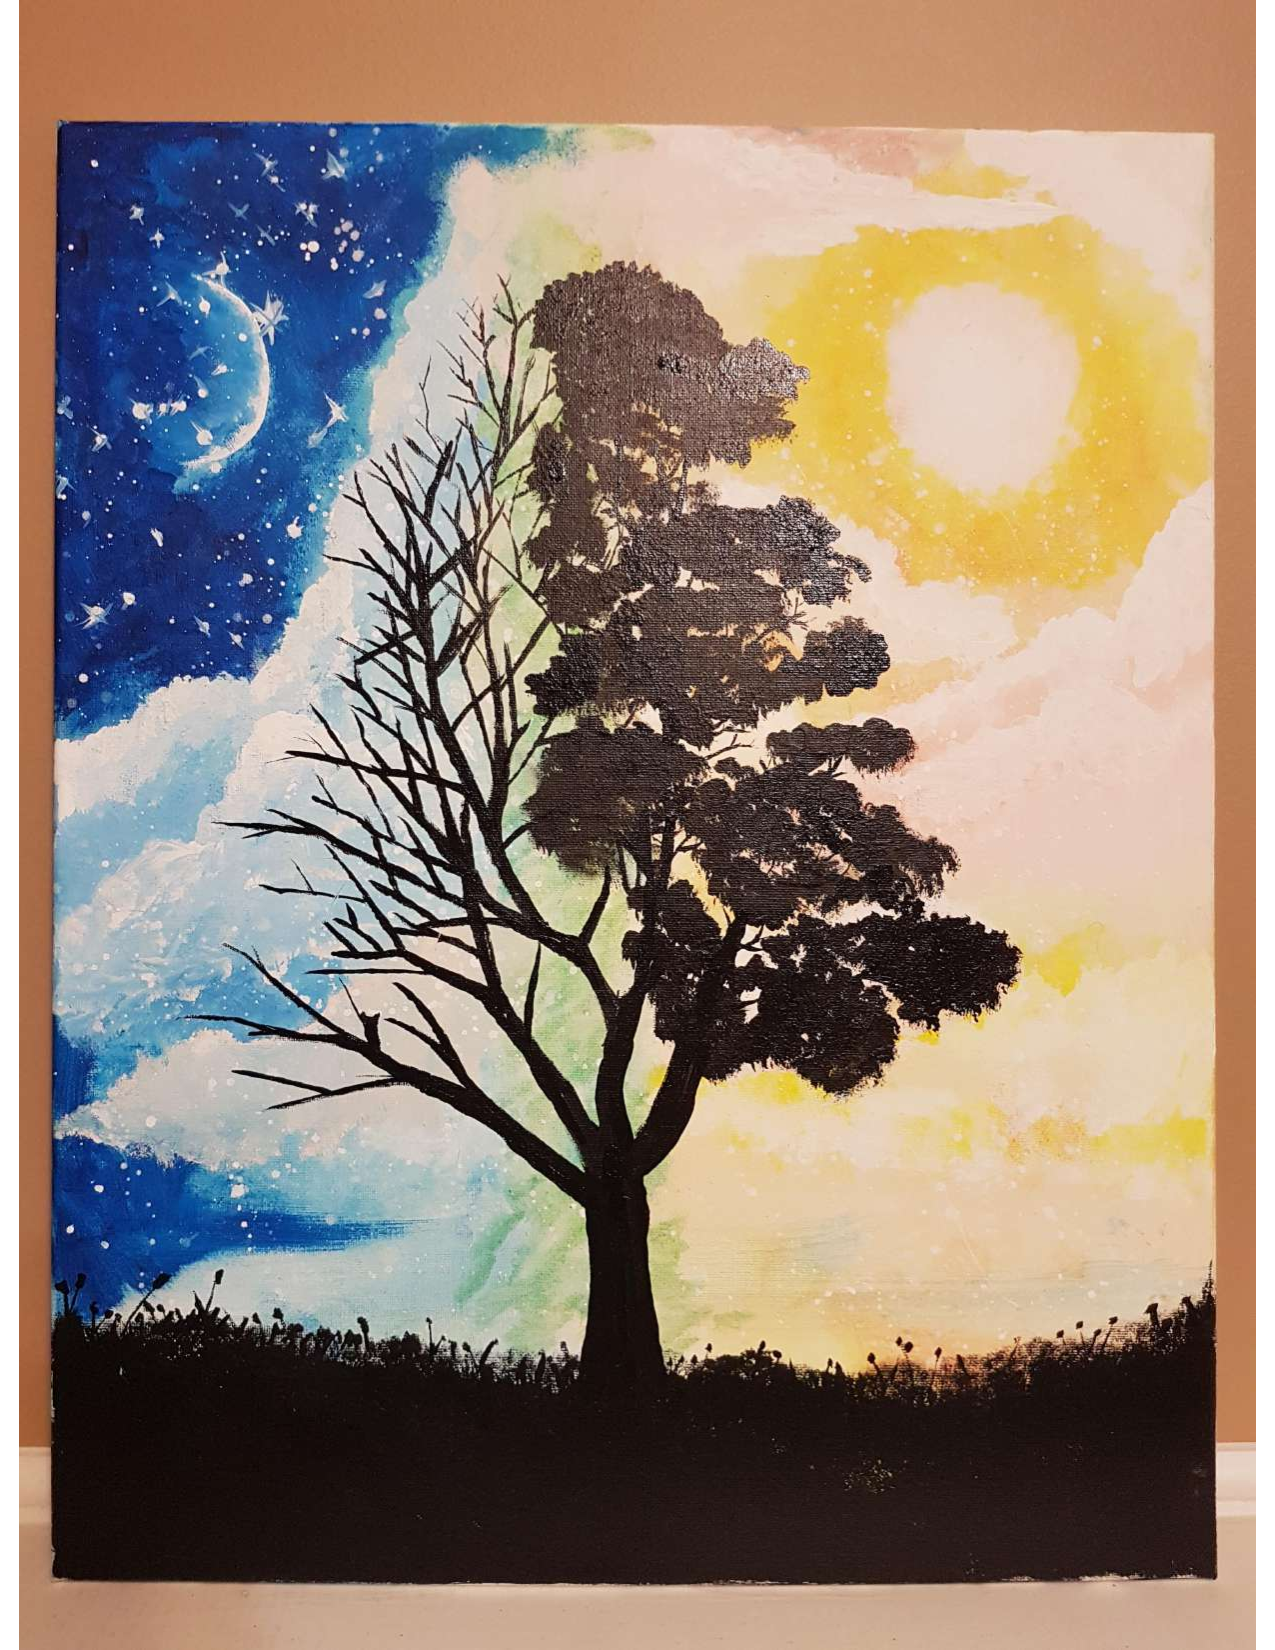
\includegraphics[width=\textwidth]{images/tree-qualitative_compressed.pdf}
    \end{minipage}
    \begin{minipage}[c]{0.8\textwidth}
\centering
\scriptsize
\begin{tabular}{p{7cm}}
\scriptsize
In this captivating painting, \textcolor{red}{a majestic tree takes center stage against a stunning backdrop. The sky above is a poetic split between night and day}—a deep, starry blue on one side with a crescent moon, and a warm, radiant blend of yellows and pinks on the other, suggesting either a sunrise or sunset. \textcolor{red}{The tree itself embodies the essence of transition}, with one side adorned in lush green foliage and the other stripped bare, \textcolor{red}{symbolizing the timeless dance of seasons and life's perpetual transformations}.

This artwork not only captures the eye but also speaks to deeper truths. It invites us \textcolor{red}{to contemplate the delicate balance between light and darkness, growth and dormancy, woven into the fabric of existence}. The artist's brushstrokes, rendered with a serene palette and gentle abstraction, evoke \textcolor{red}{a sense of tranquility and introspection}. This painting beautifully \textcolor{red}{reminds us to embrace the fleeting beauty of each passing moment, whether bathed in daylight or cloaked in the quiet mystery of night}.
\end{tabular}
\end{minipage}
\caption{Dense caption generated by Behavior-LLaVA for an artistic drawing of a tree.}
\label{fig:qualitative-image-1}
\end{figure}




\begin{figure}[t]
\begin{minipage}[c]{0.3\textwidth}
        \centering
        
\includegraphics[width=\textwidth]{images/nike-qualitative.jpeg}
    \end{minipage}
    \begin{minipage}[c]{0.72\textwidth}
\small
\centering
\scriptsize
\begin{tabular}{p{8.5cm}}\scriptsize
The image features a pair of Nike Air Force 1 sneakers, which are a classic and iconic design. The sneakers are positioned in the center of the image, with \textcolor{red}{the left shoe slightly in front of the right one, giving a sense of depth}. They are predominantly white with green accents, \textcolor{red}{including the Nike swoosh logo on the side and the outsole}. The laces are white, and \textcolor{red}{the midsole appears to be a light beige color}.

\textcolor{red}{The background is a plain, light color, which contrasts with the sneakers and makes them stand out}. Overlaid on the image is a stylized text that reads "JUST DO IT" in a cursive, flowing script. The text is in a light green color that matches the accents on the sneakers, creating a cohesive color scheme. Below the main text, there is a smaller line of text that says "New collection," indicating that these sneakers are part of a new line or series from Nike.

\textcolor{red}{The overall style of the image is clean and modern, with a focus on the product}. The use of the "JUST DO IT" slogan, which is a well-known tagline for Nike, adds a layer of branding and recognition to the image. The text is designed to be eye-catching and to \textcolor{red}{draw attention to the sneakers, which are the main subject of the image. The composition is balanced, with the sneakers centrally placed and the text evenly distributed around them}.
\end{tabular}
\end{minipage}
\caption{Dense caption generated by Behavior-LLaVA for a Nike ad. The red-colored text highlights the most important aspects of the video captured by Behavior-LLaVA, demonstrating an understanding of aesthetics, characters, world knowledge, emotion, and spatial relationships.}
\label{fig:qualitative-image-2}
\end{figure}







\begin{figure}[t]
\begin{minipage}[c]{0.32\textwidth}
        \centering
        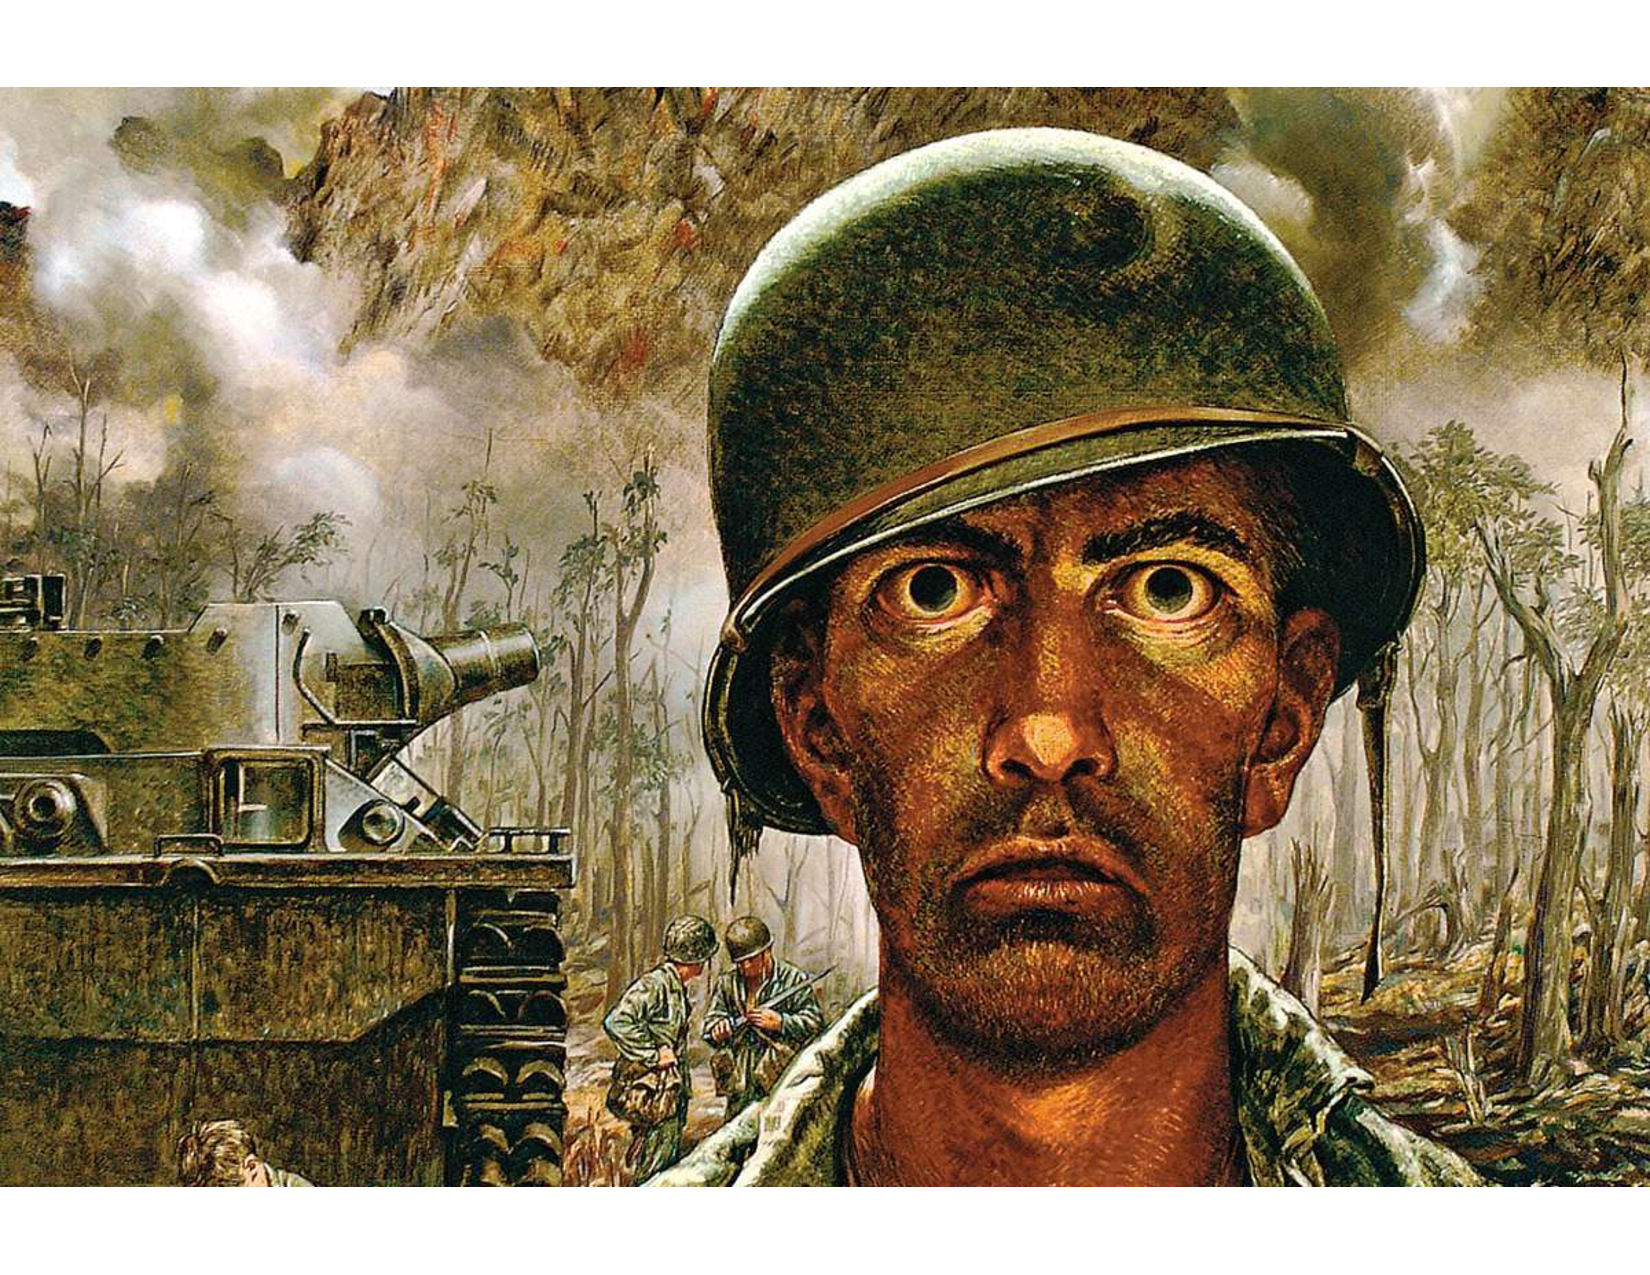
\includegraphics[width=\textwidth]{images/soldier-qualitative_compressed.pdf}
    \end{minipage}
    \hfill
    \begin{minipage}[c]{0.67\textwidth}
\small
\centering
\scriptsize
\begin{tabular}{p{8cm}}
The composition of the image presents \textcolor{red}{a compelling narrative of a soldier immersed in a war-torn landscape}. Positioned amidst a backdrop of explosive chaos and dense foliage, the soldier, adorned in traditional military gear, \textcolor{red}{gazes directly at the viewer with a resolute demeanor}. The soldier's face is camouflaged, blending seamlessly with the olive-green helmet—a hallmark of battlefield attire.

Surrounding this central figure, a tableau of activity unfolds: a tank looms in the background, its barrel skyward, suggesting recent action. Other soldiers, alert and vigilant, navigate the dense jungle terrain, underscoring the high stakes of the conflict. \textcolor{red}{The foliage, lush yet foreboding, heightens the palpable tension of the scene}.

Foregrounded by the silhouette of another soldier's helmeted head, \textcolor{red}{the viewer is drawn into the heart of the action, evoking a sense of shared experience amid the perils of warfare. The realism of the depiction accentuates the emotional weight of the moment, capturing the essence of human resilience amidst the ravages of battle.}

Overall, the image transcends mere representation, offering \textcolor{red}{a poignant reflection on the individual's role in the broader narrative of war—imbued with suspense, authenticity, and a profound exploration of the human condition within conflict.}
\end{tabular}
\end{minipage}
\caption{Dense caption generated by Behavior-LLaVA for a painting of a soldier. The model captures many qualitative aspects that are usually missed in common captioning tasks.}
\label{fig:qualitative-image-3}
\end{figure}






\begin{landscape}


\begin{figure}[t]
\begin{minipage}[c]{0.5\textwidth}
        \centering
        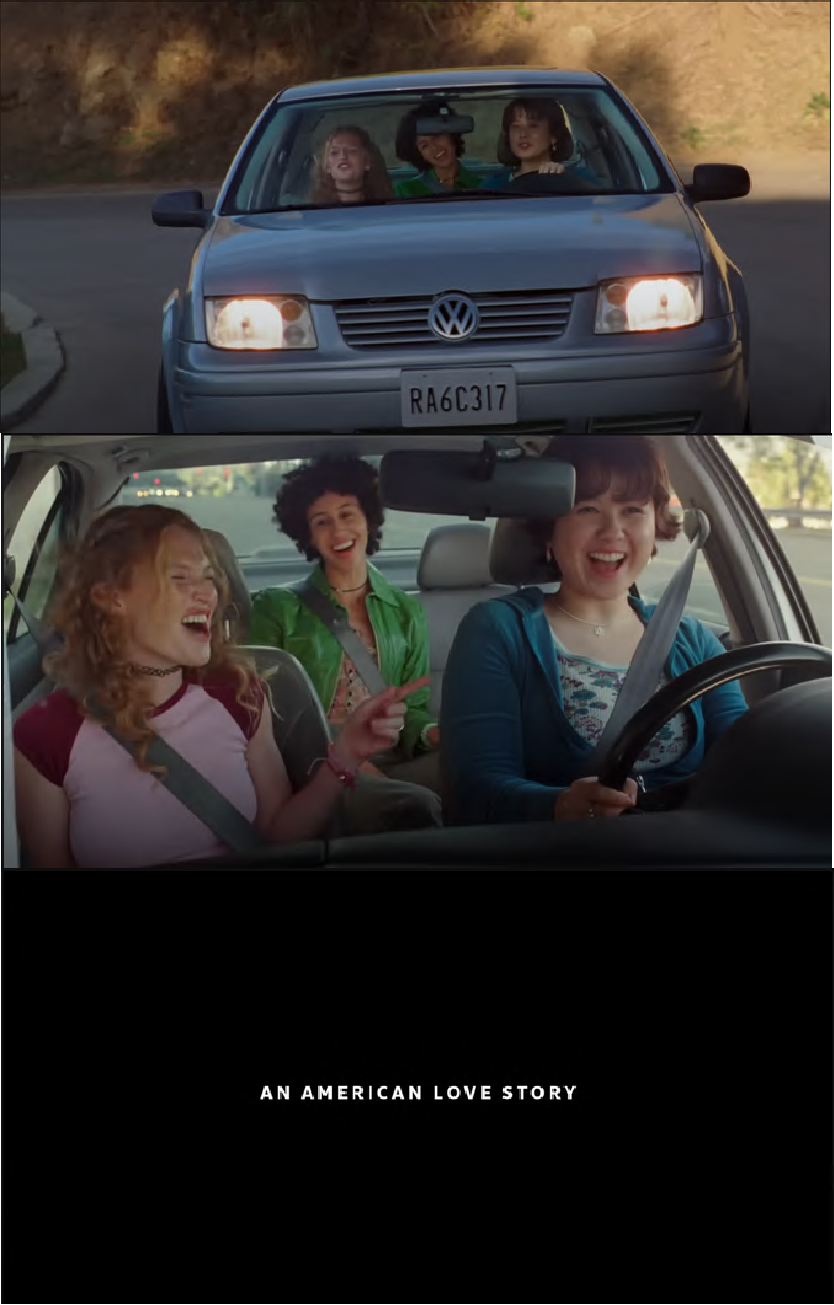
\includegraphics[width=\textwidth]{images/volswagen-video-3_compressed.pdf}
    \end{minipage}
    \begin{minipage}[c]{0.73\textwidth}
\centering
\scriptsize
\begin{tabular}{p{14cm}}\scriptsize
The Volkswagen ad titled begins with a group of three women seated excitedly in a Volkswagen Jetta, the driver sporting a wide smile as she grips the steering wheel. \textcolor{red}{The voiceover sets a nostalgic tone, likening the Jetta to unforgettable first experiences like a first kiss or hearing indie rock for the first time—a symbol of newfound freedom and excitement}.

As the scenes unfold, the camera captures the trio cruising down winding roads, their \textcolor{red}{laughter blending with the music and the wind tousling their hair. The atmosphere inside the car is one of camaraderie and adventure, with the Jetta serving as the backdrop to their shared moments of joy and spontaneity.}

Transitioning to a wider shot of the Jetta gliding along a scenic highway, surrounded by lush greenery, \textcolor{red}{the ad evokes a sense of exploration and the open road. The visuals seamlessly blend modern-day cruising with vintage footage of classic Volkswagen vehicles, reflecting on the brand's 75-year history in America, starting with the beloved Beetle.}

The ad concludes with the Volkswagen logo and \textcolor{red}{the tagline  "An American Love Story", encapsulating the enduring relationship between Volkswagen and its drivers across generations}. This phrase serves as a tribute to Volkswagen's 75-year history in America, beginning with the iconic Type 1 vehicles fondly known as "The Beetle" Through its nostalgic narrative and captivating visuals, the teaser promises viewers an immersive journey into the essence of Volkswagen—a timeless icon that has been a part of \textcolor{red}{countless cherished memories on the American road.}
\end{tabular}
\end{minipage}
\caption{Dense caption generated by Behavior-LLaVA for the video of a Volkswagen ad. The original video is posted at URL: \url{https://www.youtube.com/watch?v=kyuGXPNr-T0}. The red-colored text highlights the most important aspects of the video captured by Behavior-LLaVA, demonstrating an understanding of aesthetics, characters, world knowledge, emotion, and spatial relationships. More such examples are given in Figs.~\ref{fig:qualitative-image-1}, \ref{fig:qualitative-image-2}, \ref{fig:qualitative-image-3}, and Figs.~\ref{fig:qualitative-video-1}, \ref{fig:qualitative-video-2} for images and videos respectively. \label{fig:qualitative-video-3}}
\end{figure}







    
\begin{figure}[!t]
\begin{minipage}[c]{0.8\textwidth}
        \centering
        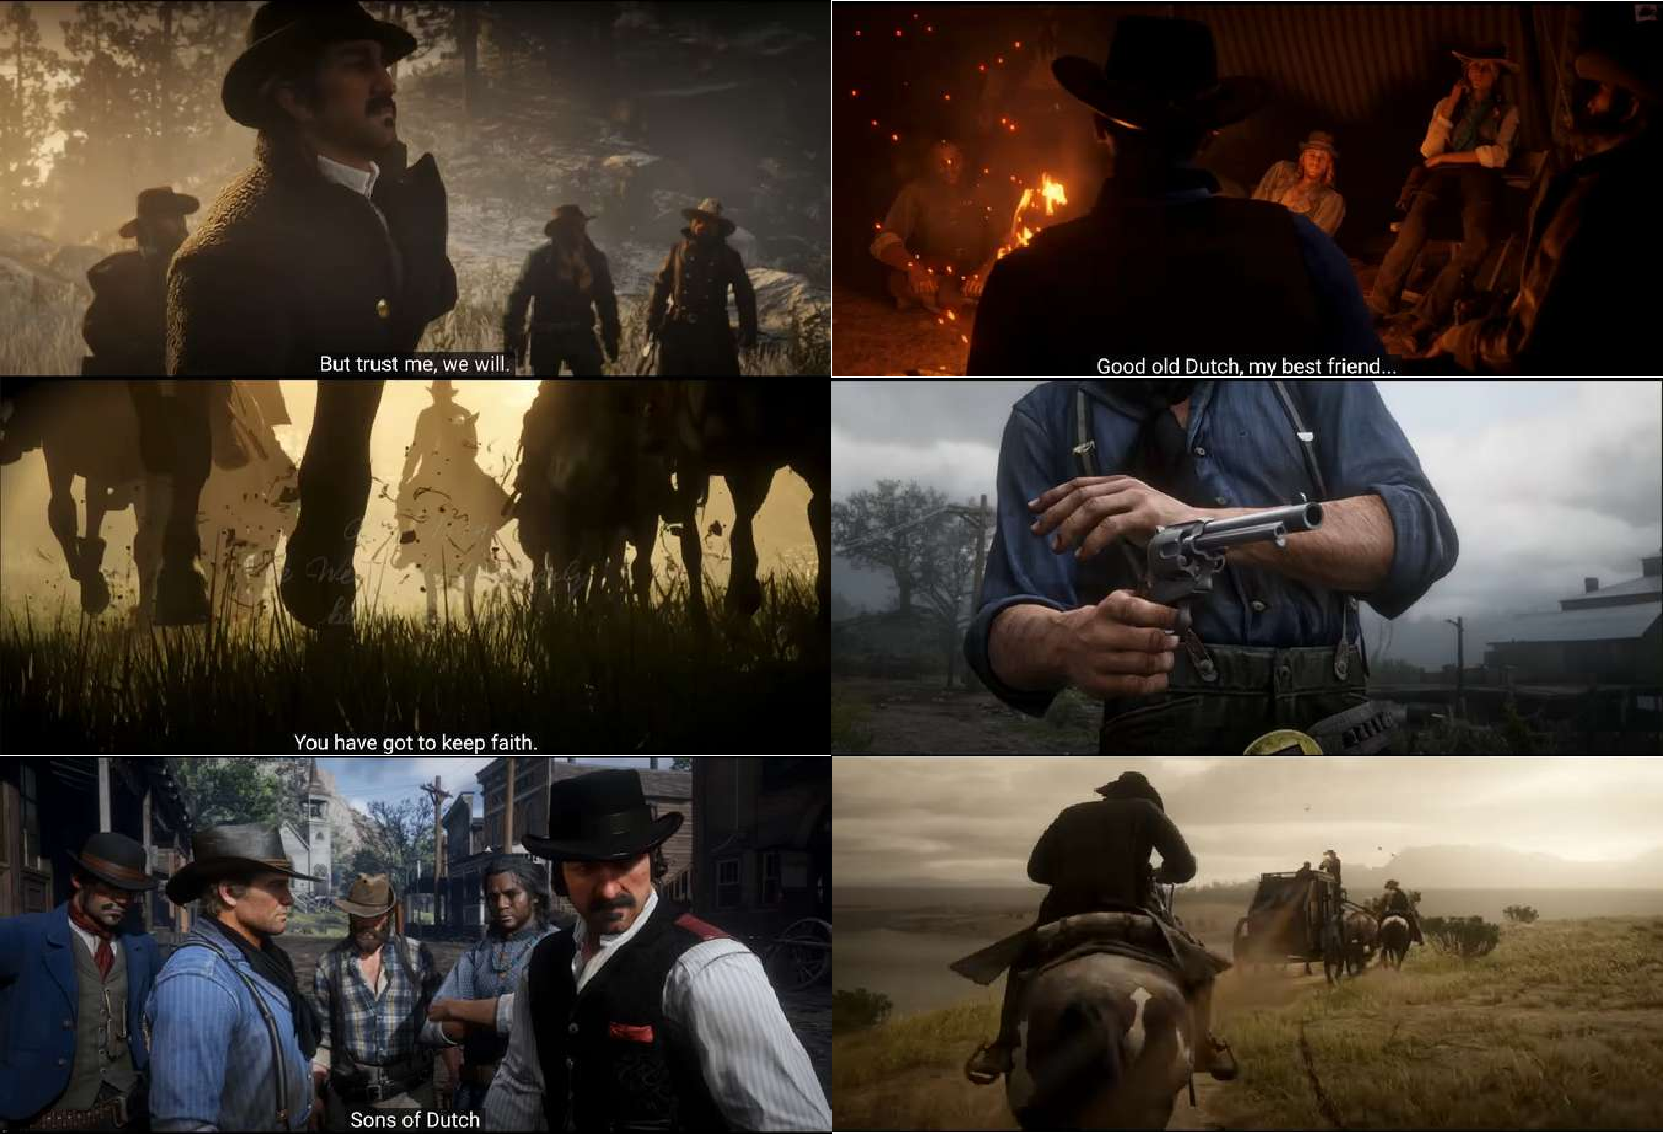
\includegraphics[width=\textwidth]{images/red-dead-game-video-1_compressed.pdf}
\end{minipage}
\begin{minipage}[c]{0.9\textwidth}
\small
\centering
\scriptsize
\begin{tabular}{p{10cm}}
In a heart-pounding and visually stunning trailer for Red Dead Redemption, \textcolor{red}{we are thrust into the gritty world of the American frontier}. The trailer opens with a voiceover, a chilling warning delivered with calm certainty: "Listen to me, we don’t want to kill any of you... But trust me, we will."

Scenes flash by in quick succession, each more intense than the last. \textcolor{red}{We see a lone figure, silhouetted against a setting sun, riding a magnificent horse through a sprawling, golden field. The rugged beauty of the landscape contrasts sharply with the impending sense of danger.}

\textcolor{red}{Cut to a dimly lit saloon where a group of hardened men sit around a table, cards in hand, tension thick in the air}. The voiceover continues, "This whole thing is pretty much done. We're more ghosts than people."

A flurry of action unfolds: a quick draw in a darkened room, \textcolor{red}{bullets slicing through the air with deadly precision}. The voiceover reminisces, "Good old Dutch, my best friend... You know how we met? A pair of hucksters trying to rob each other... Back in '78 or thereabouts."

The visuals intensify as we witness a robbery in progress, \textcolor{red}{chaos erupting as masked figures burst into a bank}. "Ladies and gentlemen, this is a robbery," declares one of the outlaws, setting the stage for a clash between lawlessness and order.

Amidst the chaos, snippets of camaraderie emerge: "Sons of Dutch. Makes us brothers." But looming shadows of betrayal and regret cast doubt on these bonds. "Sometimes, brothers make mistakes," acknowledges the voiceover, acknowledging the complexities of loyalty and survival in this unforgiving world.

\textcolor{red}{The trailer crescendos with a crescendo of gunfights, horseback chases, and impassioned speeches}. "You'll never change. I know that," declares a voice, capturing the immutable nature of the human spirit amidst adversity.

Throughout, a thematic motif resonates: "You have to love yourself a fire." \textcolor{red}{The elemental symbolism underscores the primal nature of existence in a land where survival demands courage and cunning.}

As the trailer draws to a close, we're left with the haunting refrain: "Stay strong. Stay with me." The screen fades to black, leaving us hungry for more of this epic tale set against the backdrop of the untamed West.

With breathtaking visuals and evocative storytelling, \textcolor{red}{this Red Dead Redemption trailer promises an unforgettable journey through a world where danger lurks around every corner, and the line between hero and outlaw blurs in the dust and shadows of the frontier.}
\end{tabular}
\end{minipage}
\caption{Dense caption generated by Behavior-LLaVA for the video of the official trailer of the game Red Dead Redemption 2. The original video is posted at URL: \url{https://www.youtube.com/watch?v=eaW0tYpxyp0}.}
\label{fig:qualitative-video-1}
\end{figure}




  \begin{figure}[t]
    \begin{minipage}[c]{0.7\textwidth}
            \centering
            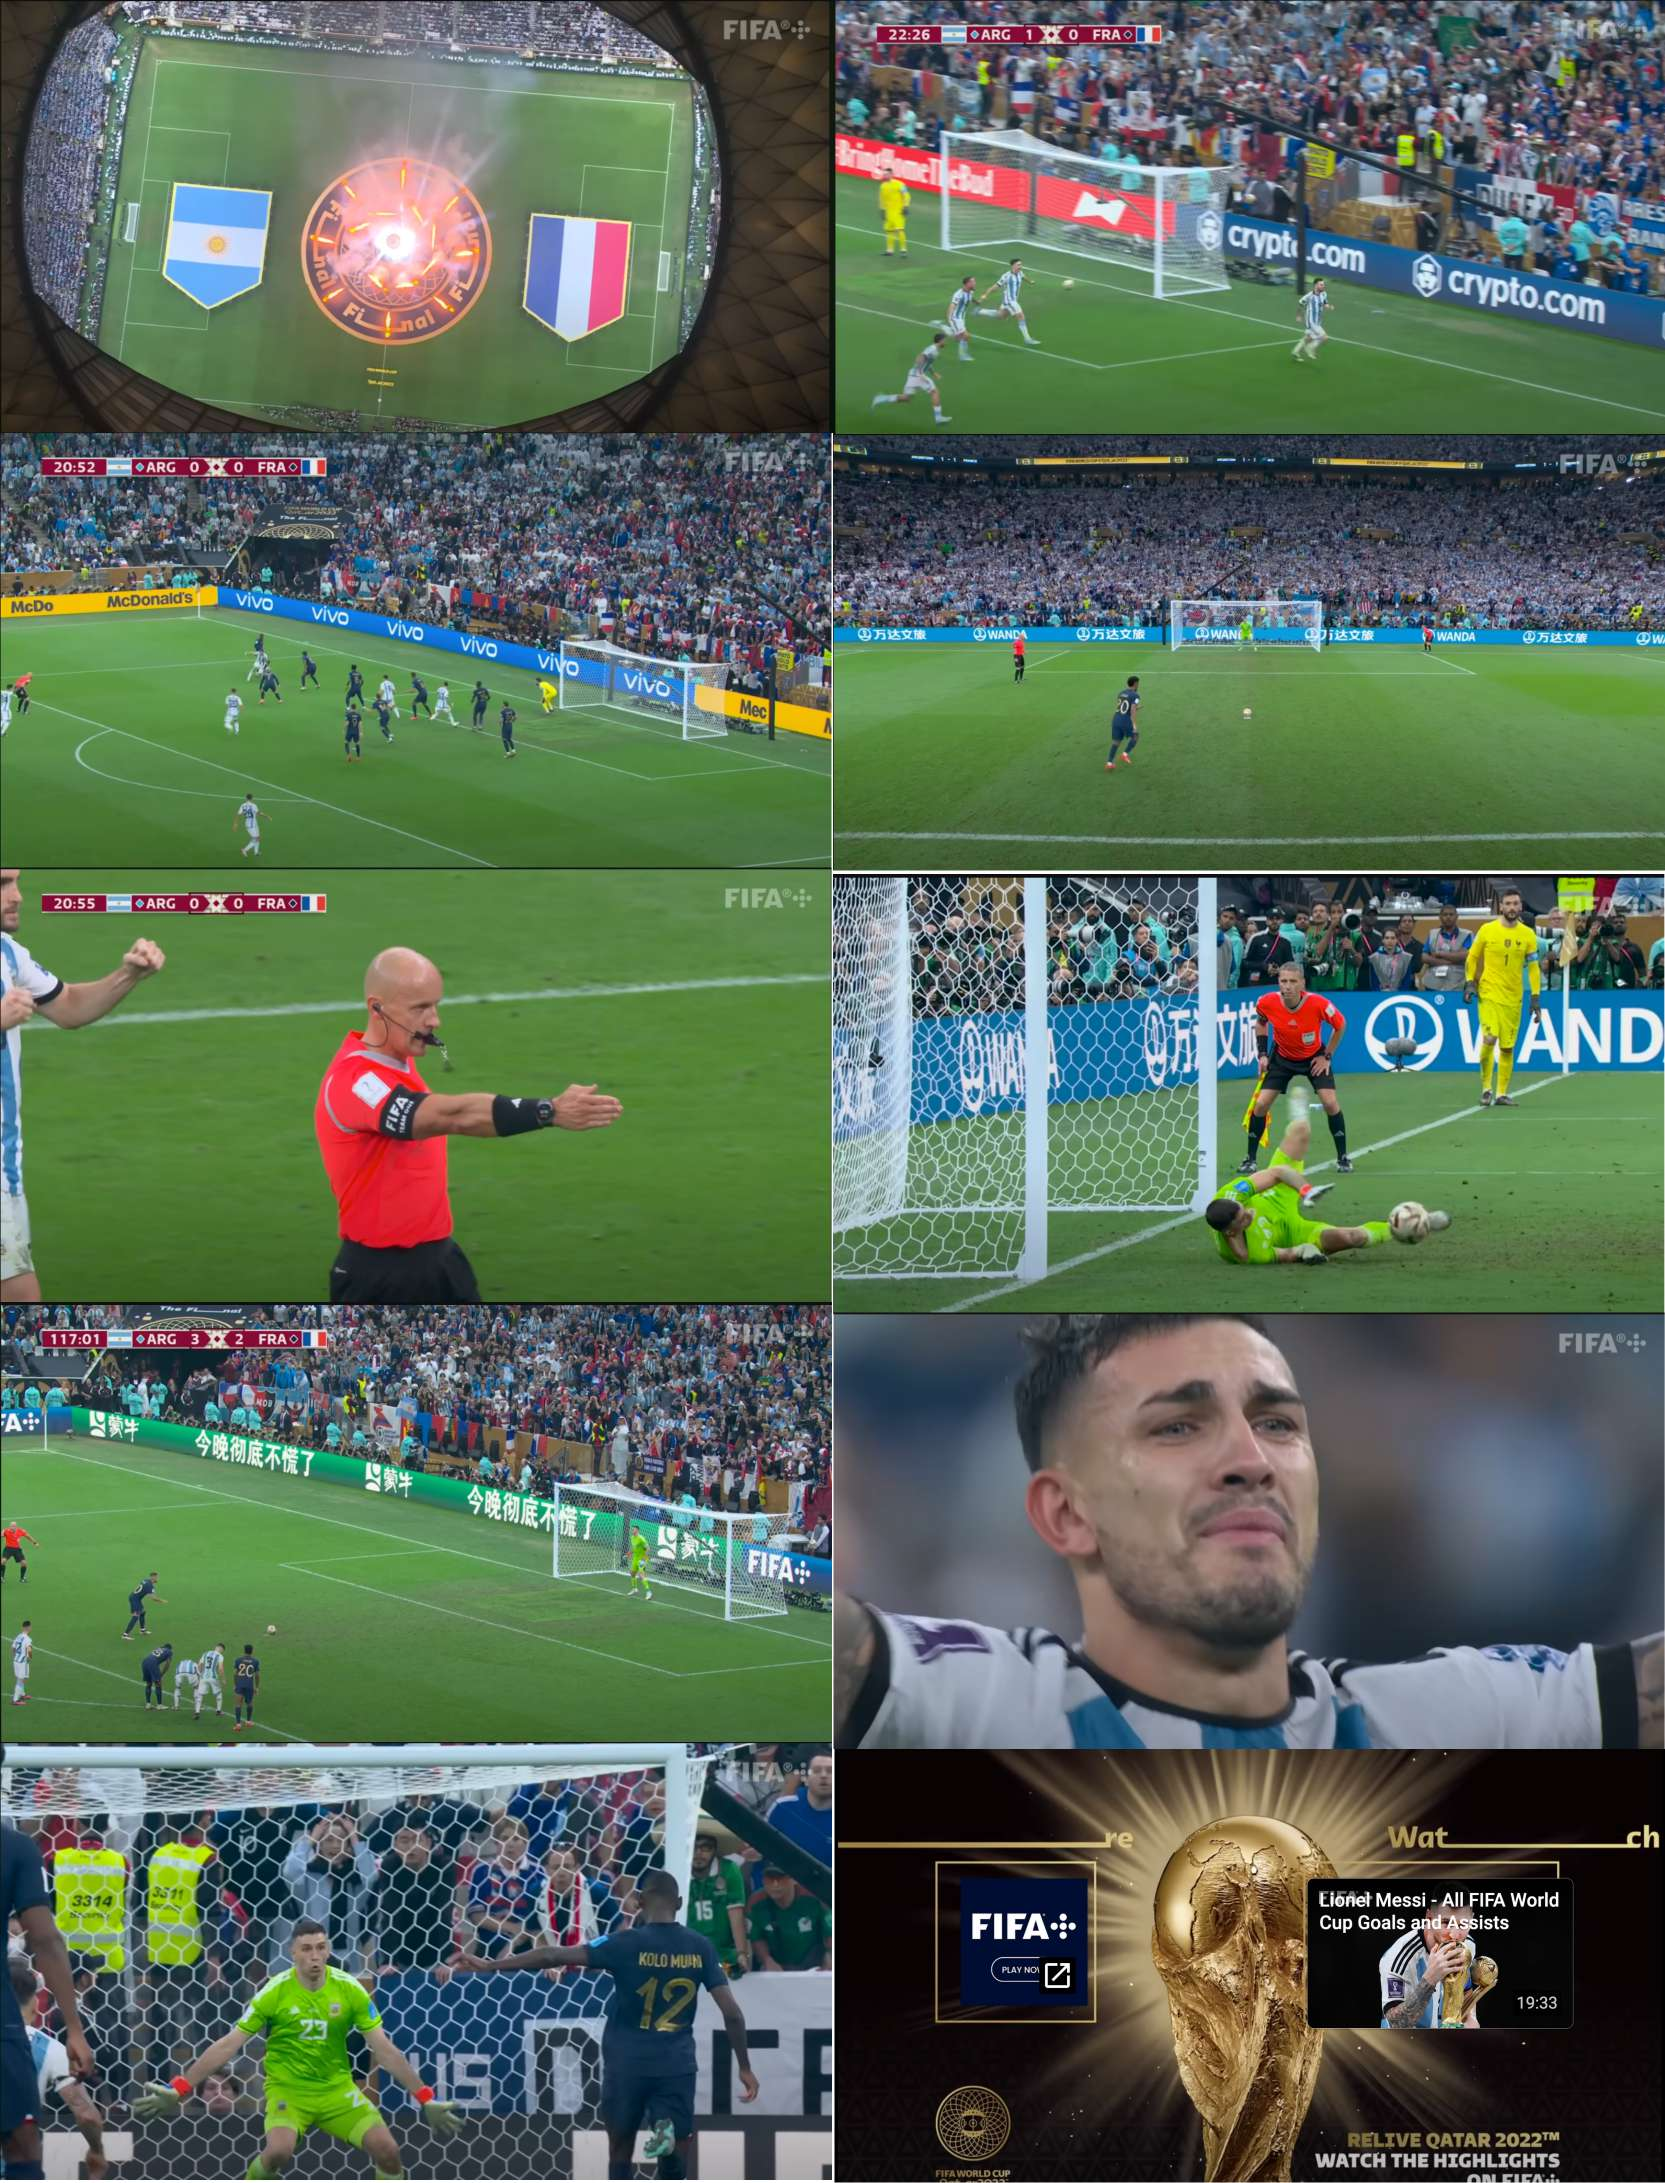
\includegraphics[width=\textwidth]{images/argentina-france-qualitative_compressed.pdf}
        \end{minipage}
        \begin{minipage}[c]{0.8\textwidth}
    \small
    \centering
    \scriptsize
    \begin{tabular}{p{12cm}}
        The scene is set at a packed stadium buzzing with excitement, the \textcolor{red}{air thick with anticipation as Argentina and France face off in what promises to be an epic World Cup final}. Lionel Messi steps up confidently to take a crucial penalty early in the match, the tension palpable as he eyes the goal. The commentator's voice echoes through the stadium, "He's got the ground, he's got a penalty! A heart beats... And Messi!" \textcolor{red}{The crowd holds its breath as Messi strikes the ball cleanly, sending it into the back of the net.} The stadium erupts with cheers as Argentina takes the lead, setting the stage for a thrilling encounter.
        
        As the game unfolds, both teams showcase their attacking prowess. Argentina's Angel Di Maria emerges as a standout, capitalizing on a swift counterattack to score a spectacular goal. "Alvarez, here's McAllister, Di Maria is the spare man, and how Di Maria! Glorious goal! Argentine gold!" The Argentine fans go wild, waving their flags and chanting passionately. However, \textcolor{red}{France fights back fiercely, earning a penalty of their own which they duly convert.}
        
        The drama intensifies in the second half as France\textcolor{red}{'s Kylian Mbappé dazzles with his speed and skill, scoring a breathtaking equalizer.} "Mbappé, to Lamp, Mbappé! Oh wow!" The match swings back and forth, with both teams pushing for victory. In the dying moments of extra time, the score is deadlocked at 3-3 when Argentina's goalkeeper makes a crucial save, denying France a late winner. \textcolor{red}{The match heads to a nail-biting penalty shootout. With nerves of steel, Argentina's players step up and convert their penalties flawlessly, culminating in a decisive save by the goalkeeper.} "Argentina, champions of the world!" The stadium erupts once more, as \textcolor{red}{Messi lifts the World Cup trophy amidst a sea of jubilant fans}, marking a historic and unforgettable victory for Argentina
    \end{tabular}
    \end{minipage}
    \caption{Dense caption generated by Behavior-LLaVA for the video of Argentina vs France FIFA World Cup Qatar 2022 Highlights. The original video is posted at URL: \url{https://www.youtube.com/watch?v=zhEWqfP6V_w}.}
    \label{fig:qualitative-video-2}
    \end{figure}

\end{landscape}









Figures~\ref{fig:qualitative-image-1}, \ref{fig:qualitative-image-2}, \ref{fig:qualitative-image-3}, and \ref{fig:qualitative-video-3}, \ref{fig:qualitative-video-1}, \ref{fig:qualitative-video-2}, show several randomly sampled qualitative examples for dense captions generated by Behavior-LLaVA over images and videos respectively. It can be noticed that despite not being explicitly trained for this task, the model performs quite well, picking up various artistic, cognitive, and object and material properties. From Table~\ref{tab:image-dense-captioning}, while Behavior-LLaVA shows a decrease in correctness over LLaMA-Vid, it shows significant improvement in other aspects, including detail and quality. On these aspects, it even comes close to 2.5X larger models (LLaVA-1.6 (34B)).

Next, in Table~\ref{tab:salicon-ablation} we compare the signals from behavioral data of perception and action. For this, we compare Behavior-LLaVA trained on BLIFT and Behaviour-LLaVA trained on Salicon salient regions and objects. Further, within BLIFT, we compare the performance from predicting singled out behaviours including likes/views, titles, comments. It can be noted that training on just Salicon results in a performance decrease for the lower-level task of action recognition (MSRVTT-QA) but improves on the higher-level task of Emotion recognition. However, the gains are smaller than those observed with training on BLIFT. 



\begin{table}[!t]
\centering
\begin{adjustbox}{max width=1.0\textwidth}
\begin{tabular}{l|ccccc}
\toprule[1.2pt]
\textbf{Model} & \multicolumn{3}{c}{\textbf{Summarization (3 Shot)}} & \textbf{Moment Retrieval} &
\textbf{Highlight Detection}\\ 
& BLEU & ROUGE & METEOR & mAP (avg) & mAP\\
\midrule[1.2pt]
Behavior-LLaVA[Replay-Graphs] & 11.2 & 19.1 & 25.3 & \textbf{35.2} & \textbf{34.9}\\
Behavior-LLaVA[Mem-Recalls] & \textbf{11.9} & \textbf{20.3} & \textbf{26.9} &34.9 & 33.1\\
Behavior-LLaVA & 10.6 & 18.3 & 22.7 & 33.1 & 32.7 \\ \midrule
LLaMA-VID & 9.1 & 16.5 & 20.3 & 30.3 & 32.4\\
Video-ChatGPT & 5.0 & 14.0 & 19.7 & - & - \\
\bottomrule[1.2pt]
\end{tabular}
\end{adjustbox}
\caption{Improvement on downstream content understanding tasks by introducing more behaviour signals. Brackets [] denote the new behaviour that we include. Replay graphs \cite{khandelwal2023large}. Mem-Recalls \cite{si2023long} Evaluation done on Multi-shot video summarization \cite{han2023shot2story20k} and MomentDETR \cite{lei2021qvhighlightsdetectingmomentshighlights}\label{tab:behavior-ablation}}
\end{table}


\subsection{Conclusion}
In this paper, we explore the idea of learning behavior leading to learning content \textit{better}. Humans produce behavior in response to content. Hence, logically, behavior should contain signals about content, which, if used as a training task, should help in learning content better. We follow this line of thought and show that training large vision and language models on user behavior data of comments and likes collected from Reddit and YouTube leads to performance improvements across a wide variety of tasks. The gains are higher on higher-level tasks such as emotion recognition, persuasion strategy classification, and question answering and smaller on lower-level tasks like action and object recognition. Further, the gains remain even after fine-tuning the VLMs on those benchmarks, thus demonstrating the importance of learning behavior in understanding content better.












%\bibliography{iclr2025_conference}
%\bibliographystyle{iclr2025_conference}















\subsection{Appendix}

\subsubsection{Listings}

\begin{lstlisting}[caption={GPT-4V Prompt to calculate correctness of a image dense caption},frame=single,breaklines=true,basicstyle=\scriptsize, label={lst:dense-caption-correctness}]
You are a great critique for analyzing images and captions.

Assess the performance of a dense image captioning model based on the correctness of the captions generated.

Please assess the correctness of the provided caption in relation to the image. Consider whether the caption accurately identifies and describes the main subjects or objects depicted in the image. Assess whether the caption correctly interprets the relationships between elements within the image, such as actions, interactions, or spatial arrangements. Focus on the precision and accuracy of the information presented in the caption. Provide a score reflecting the level of correctness, ranging from 1 (low correctness) to 10 (high correctness).
\end{lstlisting}


\begin{lstlisting}[caption={GPT-4V Prompt to calculate detail of a image dense caption},frame=single,breaklines=true,basicstyle=\scriptsize, label={lst:dense-caption-detail}]
You are a great critique for analyzing images and captions.

Assess the performance of a dense image captioning model based on the detail of the captions generated.

Evaluate the level of detail captured in the provided caption. Consider how well the caption describes specific attributes, features, or aspects of the image, including colors, shapes, textures, sizes, and any other relevant details. Assess whether the caption provides comprehensive information about the scene depicted in the image, covering both prominent and subtle elements. Pay attention to the depth and specificity of the details conveyed in the caption. Provide a score indicating the richness of detail, ranging from 1 (low detail) to 10 (high detail).
\end{lstlisting}

\begin{lstlisting}[caption={GPT-4V Prompt to calculate quality of a image dense caption},frame=single,breaklines=true,basicstyle=\scriptsize, label={lst:dense-caption-quality}]
You are a great critique for analyzing images and captions.

Assess the performance of a dense image captioning model based on the quality of the captions generated.

Assess whether the caption is concise yet descriptive, providing meaningful and engaging information about the image. Evaluate the caption's ability to evoke a clear mental image corresponding to the visual content. Additionally, consider if the caption is insightful or imaginative in its description. Provide a score reflecting the overall quality of the caption, ranging from 1 (low quality) to 10 (high quality).
\end{lstlisting}










\subsubsection{Dataset Descriptions}
\label{sec:Dataset Descriptions}
\begin{enumerate}
        \item MSVD-QA and MSRVTT-QA: These datasets are based on Microsoft Research Video Description \cite{chen2011collecting} and MSR-VTT corpora \cite{xu2016msr} and are extensively used in many video captioning and question-answering experiments. The MSVD-QA dataset has a total number of 1,970 video clips and 50,505 question-answer pairs. The MSRVTT-QA dataset contains 10K video clips and 243k question-answer pairs. 

        \item ActivityNet-QA \cite{caba2015activitynet} is a benchmark primarily for human activity understanding containing 849 hours of video, including 28,000 action instances.
        \item VideoEmotion-8 \cite{asur2010predicting} dataset comprises 1,101 user-generated videos sourced from YouTube and Flickr, each containing a minimum of 100 videos per emotional category, as per Plutchik Wheel's emotion model.
            
            \item Ekman-6 \cite{xu2016heterogeneous} dataset is compiled from social websites, with each of its 1,637 videos labeled with a single emotion category based on Ekman’s psychological research.
            
            \item CAER \cite{lee2019context} dataset, sourced from TV shows, consists of 13,201 clips with an average sequence length of 90, each manually labeled with six basic emotions, aligning with the Ekman-6 dataset. 

            \item IAPSa \cite{mikels2005emotional} is a subset of IAPS, following the Mikels model with eight emotion categories such as amusement, awe, contentment, excitement, anger, disgust, fear, and sadness. It consists of 395 affective images, marking the first visual emotion dataset with discrete categories.
            
            \item Emotion6 \cite{peng2015mixed} features 1,980 images sourced from Flickr, each labeled by 15 annotators according to the Ekman model, covering six emotion categories: happiness, anger, disgust, fear, sadness, and surprise.
            \item EmoSet \cite{yang2023emoset} encompasses a total of 3.3 million images, including 118,102 from social networks and artistic sources, evenly distributed across various emotion categories. Based on the Mikels model, EmoSet is categorized into eight emotion categories.
            \item Abstract \cite{machajdik2010affective} exclusively consists of color and texture combinations without recognizable objects. Differing from the IAPS dataset where emotions often stem from identifiable objects, the abstract paintings dataset was peer-rated via a web survey, with each image rated approximately 14 times. It comprises 228 images spanning eight categories similar to those in IAPS.


                     \item Memento10k\cite{newman2020multimodal} is a short-term video memorability dataset comprising 10,000 video clips,  with 900,000 human memory annotations recorded at various delay intervals. The video clips were, on average, 3s long.
            \item VideoMem \cite{cohendet2019videomem} is comprised of 10,000 soundless videos, each lasting 7 seconds, accompanied by memorability scores. Memorability was measured twice: first, shortly after viewing and again 24-72 hours later to capture both short-term and long-term memorability effects.
            \item LaMem \cite{khosla2015understanding} dataset is a short-term image memorability dataset comprising of 60000 images. The dataset contains scene-centric images, object-centric images and other types such as images
            of art, images evoking certain emotions, and other user-generated images.
            \item SUN \cite{isola2011makes} dataset is a short-term image memorability dataset comprising 2222 images that were sourced from the SUN database. 
   
         \item MemCat \cite{goetschalckx2019memcat} dataset is a short-term image memorability dataset comprising 10000 images. It consists of five broader memorability-relevant semantic categories (animal, sports, food, landscapes, vehicles), with 2K exemplars each, further divided into different subcategories (e.g., bear, pigeon, cat, etc. for animal). The images were sourced from existing image sets: ImageNet, COCO, Open Images Dataset, and SUN. 
            \item MediaEval \cite{Kiziltepe2021} utilized publicly available links to short-form video clips, each averaging 6 seconds in duration, with both short-term and long-term memorability scores. Short-term memorability evaluations were conducted on videos viewed within the preceding few minutes, while long-term memorability assessments were based on videos viewed within the previous 24 to 72 hours.
            \item LAMBDA \cite{si2023long} is a long-term memorability consisting of 2205 video ads collected over 1749 participants covering 276 brands. The average video length is 33 seconds and the videos are highly complex, consisting of audio, logos, fast-moving scenes, emotions, \textit{etc}.
\end{enumerate}


\subsubsection{Limitations}
In this paper, we try to show the hypothesis that training on the behavior modality improves learning of the content modality. We train the models on comments and likes to show this. We test our models on multiple benchmarks and obtain positive results. While we try to cover a wide variety of tasks and while results do conclusively show that the hypothesis is true, yet, we can test on more benchmarks covering even more tasks. Similarly, we can show it with multiple models, other than LLaMA-Vid.


\subsection{Broader Impacts}
Our paper talks about how behavioral training can positively impact content understanding of VLMs. We think this will be useful in various content understanding applications such as question answering, captioning, etc. 

\subsubsection{Ethical Implications}

This paper demonstrates that training on behavioral modalities enhances the learning of content modalities. Models trained on user interactions such as comments and likes were tested on multiple benchmarks and yielded positive results. While these findings present exciting opportunities for advancing content understanding in AI systems, they also raise important ethical considerations that must be carefully addressed.

1.~No personally identifiable information (PII) is used to improve content understanding. Instead, aggregated behavioral data, including replays, likes, and comments, is utilized, ensuring user privacy. We have implemented rigorous anonymization and aggregation techniques to protect individual user identities. 

2.~We explicitly acknowledge the inherent biases that may exist in data sourced from social media platforms such as Reddit and YouTube. Despite our rigorous data filtering and cleaning processes, we recognize that the dataset may still be subject to demographic skews, self-selection bias, and algorithmic influences. These biases could potentially lead to uneven model performance across different user groups or reinforce existing societal biases.
To mitigate these issues, we emphasize the importance of considering these broader implications when applying our model and interpreting its results. 


3.~We acknowledge the need for greater cultural diversity in our dataset. To address this, we plan to release our artifacts as open-source and encourage community contributions to incorporate multilingual and multicultural data. This could involve expanding the range of subreddits and YouTube channels included in our dataset, with the aim of capturing a more diverse and representative spectrum of receiver behavior across different cultural contexts.
By taking this approach, we hope to enhance the ethical considerations and societal impact of our work, providing a more holistic view of behavioral patterns in various cultural settings. However, we also recognize that this approach may introduce new challenges, such as ensuring the quality and reliability of community-contributed data.

